\documentclass[12pt,twoside]{Book} 
% \usepackage[a4paper,tmargin=1.5cm, bmargin=2cm, lmargin=1.5cm, rmargin=1.5cm]{geometry}
\usepackage[a4paper,tmargin=2cm, bmargin=2.5cm, lmargin=3.5cm, rmargin=2.0cm]{geometry}
\usepackage{color,calc,graphicx,soul,fourier}  
\usepackage{graphicx}
\usepackage{amsmath,amssymb,latexsym,amsfonts, bbm,mathtools, enumitem,esvect,commath,pifont}
\usepackage[backend=biber, style=alphabetic, sorting=ynt]{biblatex}
\usepackage{fourier}
\usepackage{titling}
\usepackage{longtable}
\usepackage{gensymb}
% \usepackage[utf8]{vietnam}
\usepackage{afterpage}
\usepackage{enumitem}
\usepackage{xparse}
\usepackage{tabvar}
\usepackage{titlesec} 
\usepackage{lipsum}
\usepackage{tikz,pgf,tkz-tab}
\usepackage{multicol}
\usepackage{pdfpages}
\usepackage{fancyhdr}
\usepackage{xparse}
\usepackage{hyperref}
\usepackage{chngcntr}
\usepackage[absolute,overlay]{textpos}
\usepackage{float}
\pagestyle{fancy}
\lhead[]{}\chead[]{}\rhead[]{}
\lfoot[\sl Page \thepage]{
    \it Electronic Device Component
    \hfil 
}
\cfoot[]{}
\rfoot[\it HCMUT - Computer Engineering]{\sl Page \thepage}
\renewcommand{\headrulewidth}{0pt}
\renewcommand{\footrulewidth}{1pt}  
\setlength{\parindent}{0pt}
\newcommand{\debugline}{\vspace{-0.5cm}\phantom{Debug error no line to end}}
\newcommand\blankpage{%
    \null
    \thispagestyle{empty}%
    \addtocounter{page}{0}%
    \newpage}

\newcommand*{\TitleFont}{%
      \usefont{\encodingdefault}{\rmdefault}{b}{n}%
      \fontsize{40pt}{50pt}%
      \selectfont}

\titleformat{\chapter}[display]
  {\bfseries\Huge}
  {\filright\MakeUppercase{\chaptertitlename} \Huge\thechapter}
  {2ex}
  {\titlerule\vspace{1ex}\filleft}
  [\vspace{1ex}\titlerule]
  
\addbibresource{references.bib} %Imports bibliography file

% Input definition for questions
\newcounter{question}
\newif\ifinchoices
\inchoicesfalse
\newenvironment{questions}{%
  \list{\thequestion.}%
  {%
    \usecounter{question}%
    \def\question{\inchoicesfalse\item}%
    \settowidth{\leftmargin}{10.\hskip\labelsep}%
    \labelwidth\leftmargin\advance\labelwidth-\labelsep
  }%
}
{%
  \endlist
}%

\newcounter{choice}
\renewcommand\thechoice{\Alph{choice}}
\newcommand\choicelabel{\thechoice.}
\def\choice{%
  \newline
  \ifinchoices
    % Do nothing
  \else
    \startchoices
  \fi
  \refstepcounter{choice}%
%   \ifnum\value{choice}>1\relax
%   \penalty -50\hskip 1em plus 1em\relax
%   \fi
  \choicelabel
  \nobreak\enskip
}% choice
\def\CorrectChoice{%
  \choice
  \addanswer{\thequestion}{\thechoice}%
}
\let\correctchoice\CorrectChoice

\newcommand{\startchoices}{%
  \inchoicestrue
  \setcounter{choice}{0}%
% \par % Uncomment this to have choices always start a new line
  % If we're continuing the paragraph containing the question,
  % then leave a bit of space before the first choice:
  \ifvmode\else\enskip\fi
}%

\counterwithin*{section}{chapter}
\counterwithin*{subsection}{section}
\counterwithin*{subsubsection}{subsection}

\newbox\allanswers
\setbox\allanswers=\hbox{}
\newcommand{\addanswer}[2]{%
  \global\setbox\allanswers=\hbox{\unhbox\allanswers #1.~#2\quad}%
}
\newcommand{\showanswers}{%
  \vfill
  \begin{center}
    Đáp án
  \end{center}
  \noindent\unhbox\allanswers
}

\begin{document}
\thispagestyle{empty}
\AddToShipoutPictureBG*{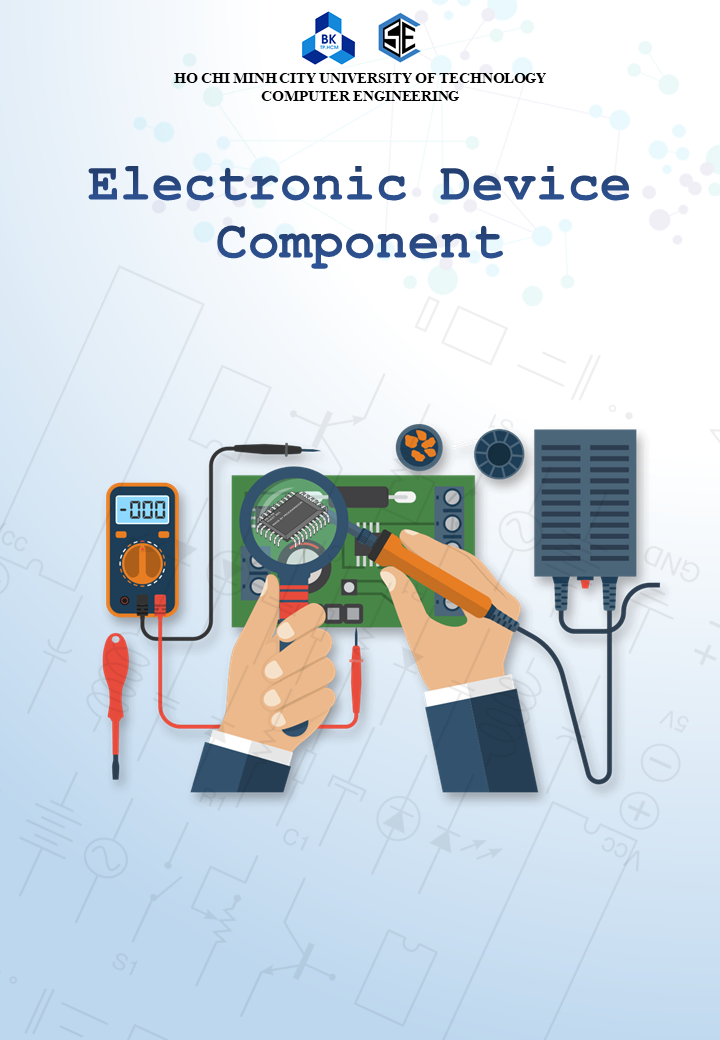
\includegraphics[width=\paperwidth,height=\paperheight]{source/picture/cover.png}}

\begin{textblock*}{22cm}(0cm,27cm)
\begin{center}
    \textbf{Dr. Le Trong Nhan}
\end{center}
\end{textblock*}

\thispagestyle{empty}
\debugline
\newpage

\thispagestyle{empty}
\debugline
\newpage

\thispagestyle{empty}
\begin{center}
\bf{\Large }
\end{center}

\afterpage{\blankpage}

\tableofcontents

%\chap{First Project on PSpice}

\section{Introduction}
PSpice for TI is a design and simulation environment that helps evaluate functionality of analog circuits. This full-featured, design and simulation suite uses an analog analysis engine from Cadence®. Available at no cost, PSpice for TI includes one of the largest model libraries in the industry, spanning our analog and power portfolio, as well as select analog behavioral models.\\

The PSpice for TI design and simulation environment allows you to simulate complex mixed-signal designs with its built-in library. Create complete end equipment designs and prototype your solutions before you commit to layout and fabrication, reducing time to market and development cost. \\

Within the PSpice for TI design and simulation tool, you can search for TI devices, explore the portfolio, open test benches and simulate your design to further analyze the selected device. You can also run co-simulation of multiple TI devices to better represent your system.\\

In addition to a full library of preloaded models, you can easily access the latest technical collateral for TI devices within the PSPICE-FOR-TI tool. After you have verified that you have the correct device for your application, you can access the TI store to purchase the product. Using PSpice for TI, you have access to tools to address your simulation needs as you progress through the design cycle, from circuit exploration to design development and verification. Available at no cost, it is easy to get started.\\

A primary purpose of this lab is for you to become familiar with the use of PSpice and to learn to use it to assist you in the analysis of circuits (e.g. double check the results with your exercise). The software is required to  install in your computer. Moreover, it is your responsibility to learn its use in a more detailed way since you will be using it along the course of this semester and in the future.
The targets in the first manual are summarized as follows:
\begin{itemize}
    \item PSpice installation on Windows OS
    \item Create a project on PSpice
    \item Create a bias analysis profile
    \item Run the simulation and obtain results
\end{itemize}
\newpage
\section{PSpice installation}
The homepage to install this tool is located at \link{https://www.ti.com/tool/PSPICE-FOR-TI}.
\begin{figure}[!htp]
    \centering
    
\includegraphics[width=4in]{source/picture/bai_1/pic1.PNG}
    \caption{\textit{Homepage to download PSpice}}
    \label{bai1_pic1}
\end{figure}

By clicking on the \textbf{Download} button, the website is navigated as follows:
\begin{figure}[!htp]
    \centering
    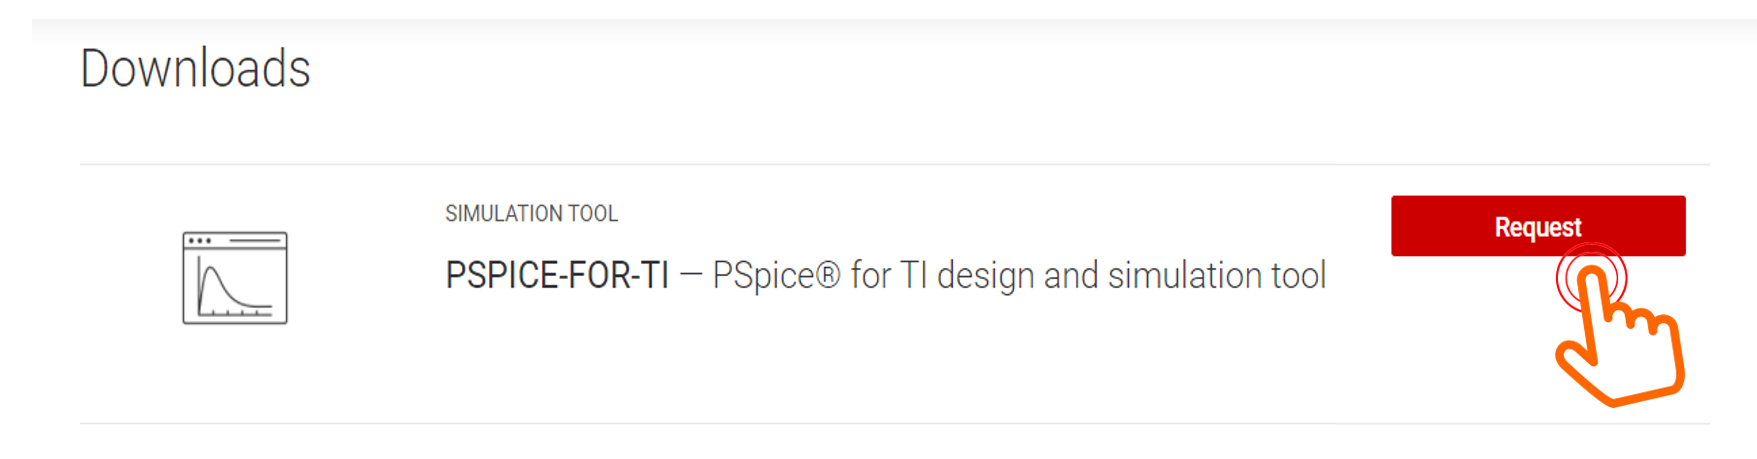
\includegraphics[width=4in]{source/picture/bai_1/pic2.PNG}
    \caption{\textit{Request information for downloading}}
    \label{bai1_pic2}
\end{figure}

Basically, you need to login before requesting a setup file. Please follow the manuals from the website to accomplish this process. An email with an access key will be sent to your account to activate the PSpice software.

\section{Create a project on PSpice}
\textbf{Step 1: } Launch PSpice for TI from windows start menu.
\begin{figure}[!htp]
    \centering
    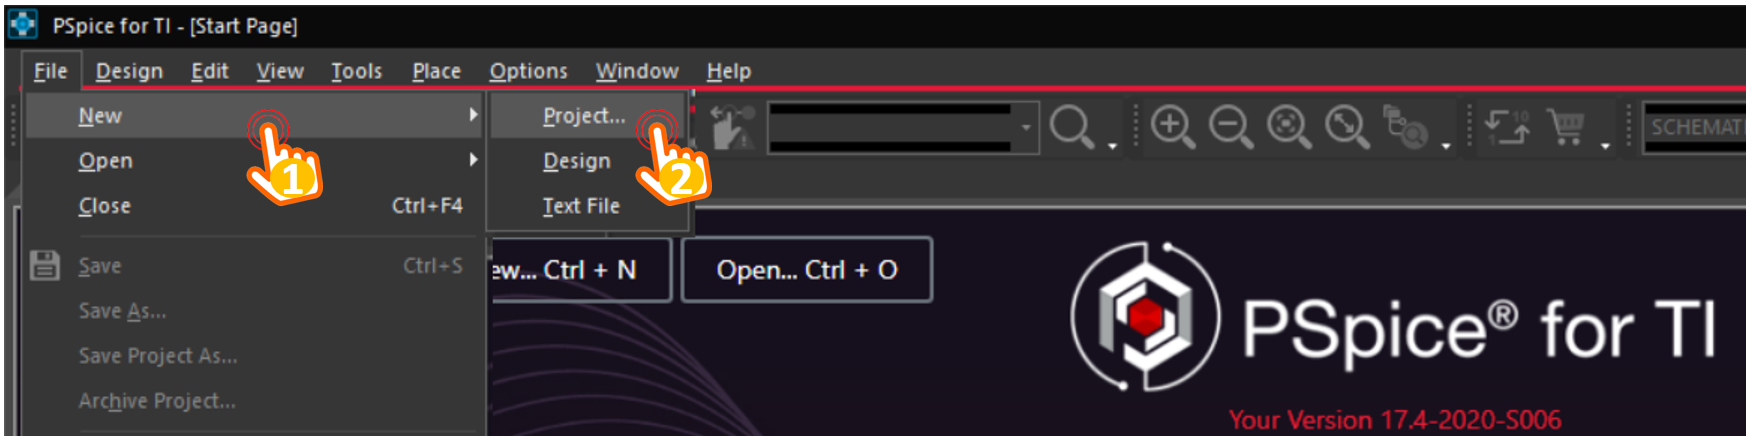
\includegraphics[width=4in]{source/picture/bai_1/pic4.PNG}
    \caption{\textit{Create a new project on PSpice}}
    \label{bai1_pic4}
\end{figure}

From menu \textbf{File}, select \textbf{New}, then select \textbf{Project}.

\textbf{Step 2: } Create an empty project as follows.
\newpage
\begin{figure}[!htp]
    \centering
    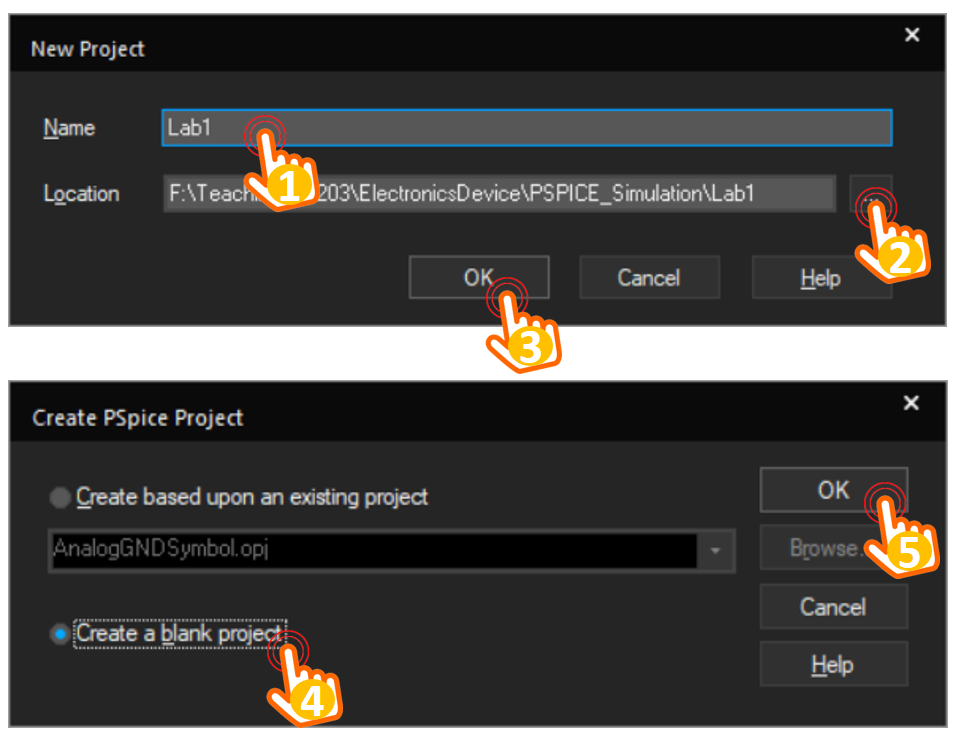
\includegraphics[width=4in]{source/picture/bai_1/pic5.PNG}
    \caption{\textit{Provide the name, location and select a blank project}}
    \label{bai1_pic5}
\end{figure}

In the second dialog, please select \textbf{Create a blank project}. An empty project is created and the next UI is displayed as follow.
\begin{figure}[!htp]
    \centering
    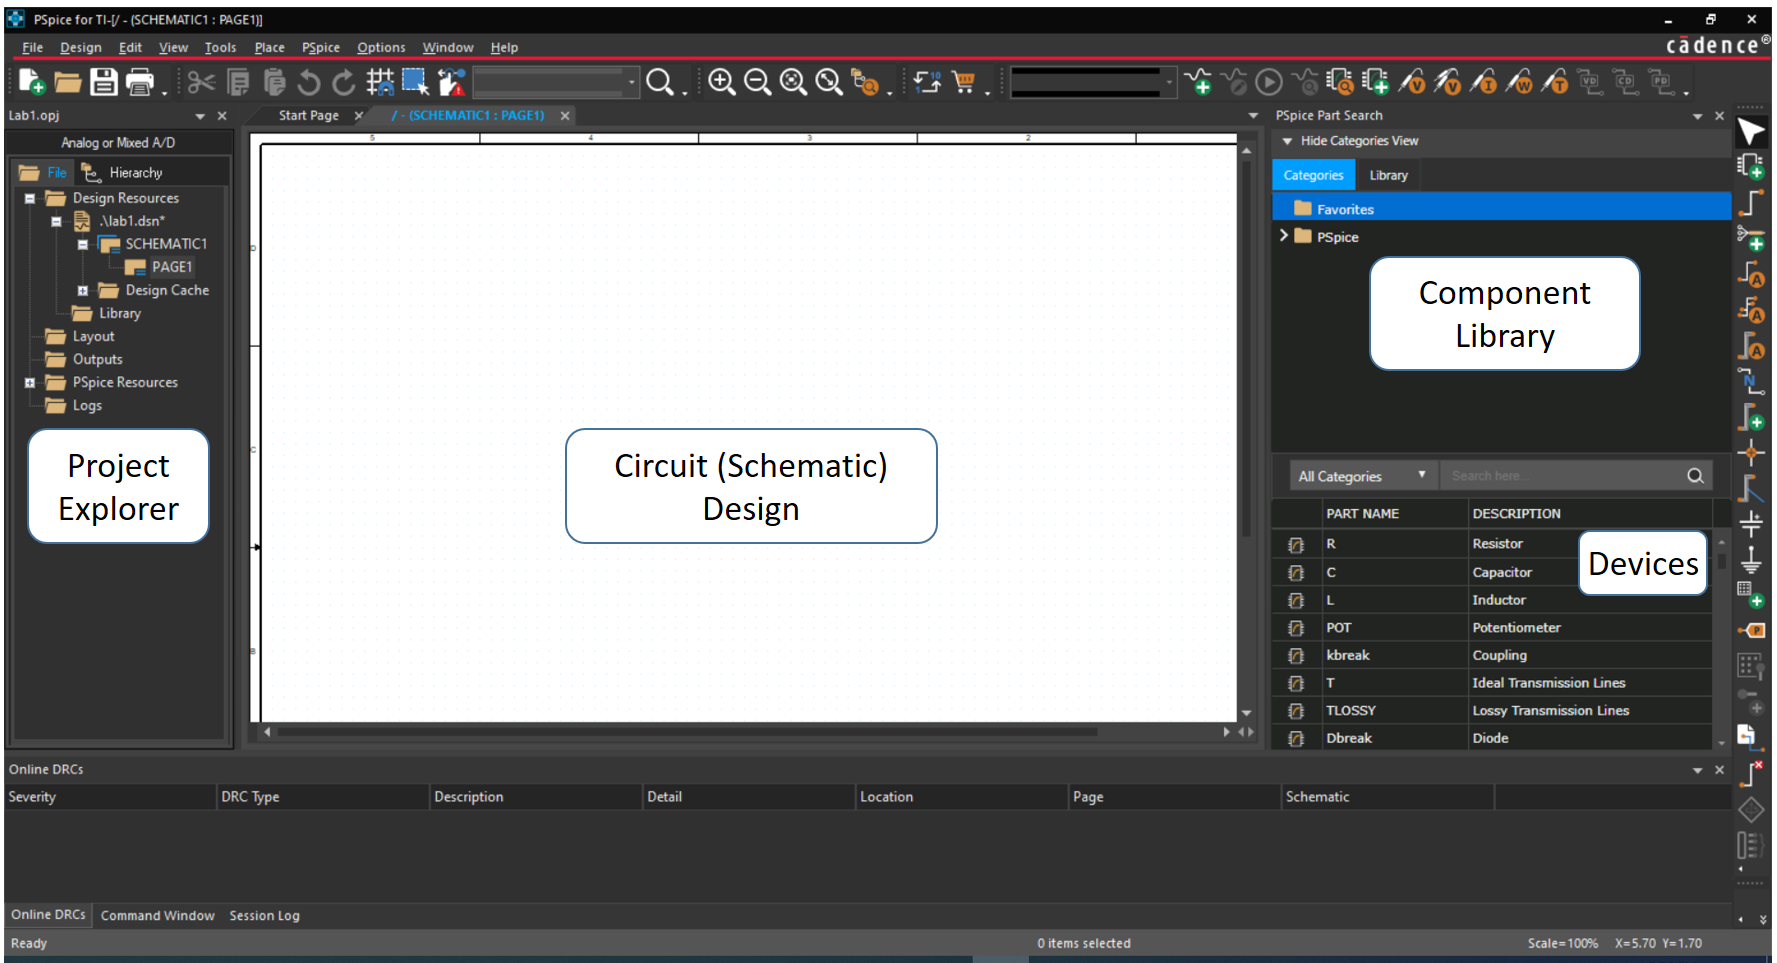
\includegraphics[width=5.5in]{source/picture/bai_1/pic3.PNG}
    \caption{\textit{An empty project is created on PSpice}}
    \label{bai1_pic3}
\end{figure}

\section{Design a circuit}

\textbf{Step 1: } Double click on the Resistor in the device list and then move the mouse to the schematic design page. This device is in the \textbf{Favourite} library in default. While moving, \textbf{press R} to rotate the device before placing it (by left-mouse click), as follow:

\begin{figure}[!htp]
    \centering
    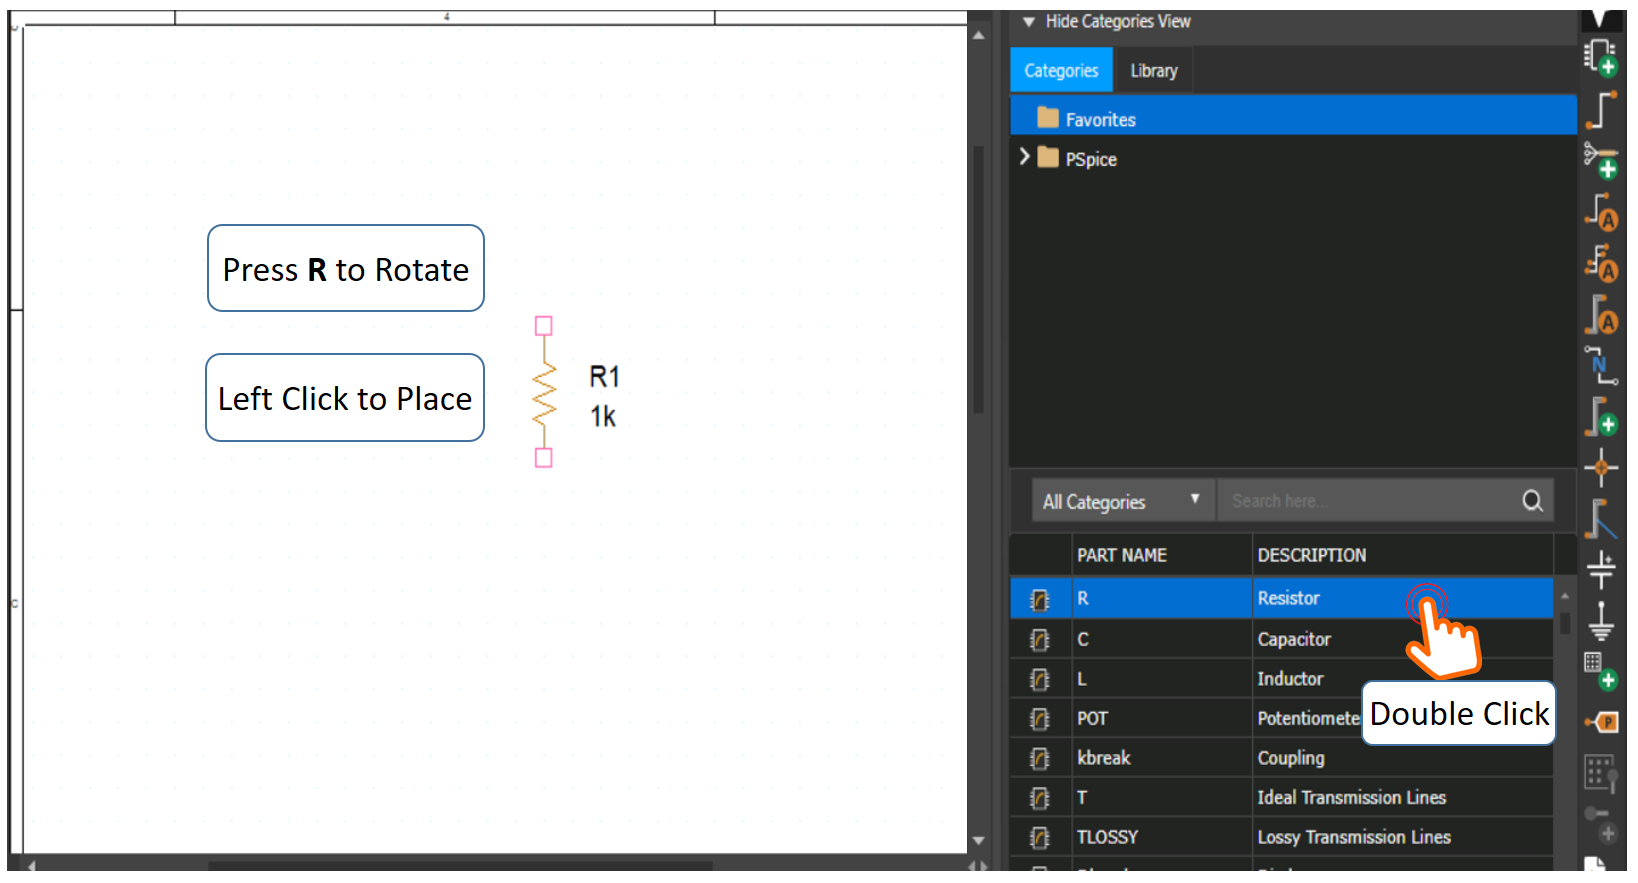
\includegraphics[width=4in]{source/picture/bai_1/pic6.PNG}
    \caption{\textit{Place a resistor in PSpice}}
    \label{bai1_pic6}
\end{figure}

\newpage
\textbf{Step 2: } Double click on the value of the resistor, which is 1k in default, in order to change its resistance.

\begin{figure}[!htp]
    \centering
    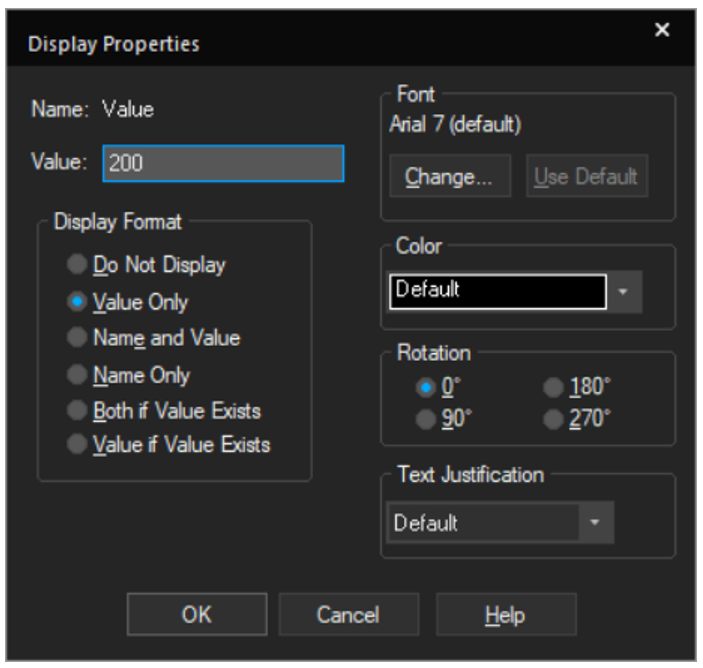
\includegraphics[width=3in]{source/picture/bai_1/pic7.PNG}
    \caption{\textit{Assign the resistance}}
    \label{bai1_pic7}
\end{figure}

If the resistance is Ohm, no unit is required in the \textbf{Value} field. Repeat the first 2 steps to finalize all resistors in the circuit.

\begin{figure}[!htp]
    \centering
    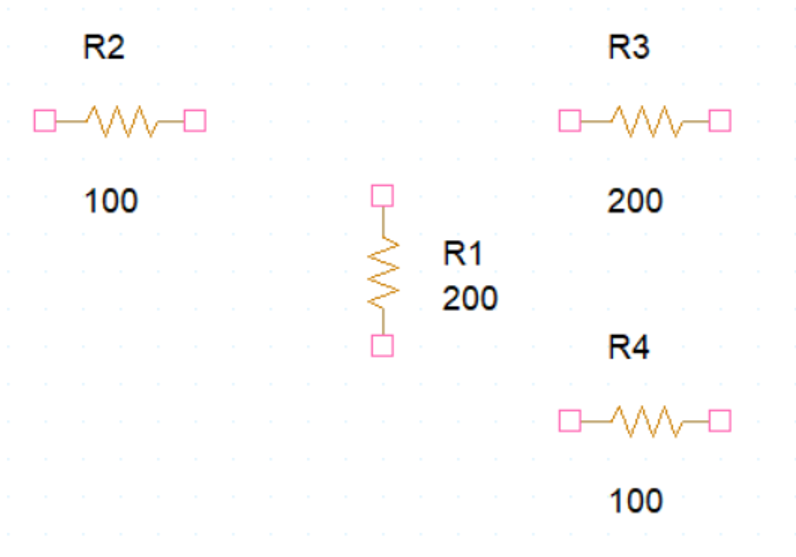
\includegraphics[width=3in]{source/picture/bai_1/pic8.PNG}
    \caption{\textit{Place other resistors in PSpice}}
    \label{bai1_pic8}
\end{figure}

Some hot keys including \textbf{Ctrl + C} and \textbf{Ctrl + V} can be used to copy an old device.\\

\textbf{Step 3: } In order to place a voltage supple, find the component named \textbf{VDC} (DC Voltage Source) in the favourite list, or filter it on the search area. Double click on the voltage supply and change to a desired value. The result after this step is expected as figure bellow.

\begin{figure}[!htp]
    \centering
    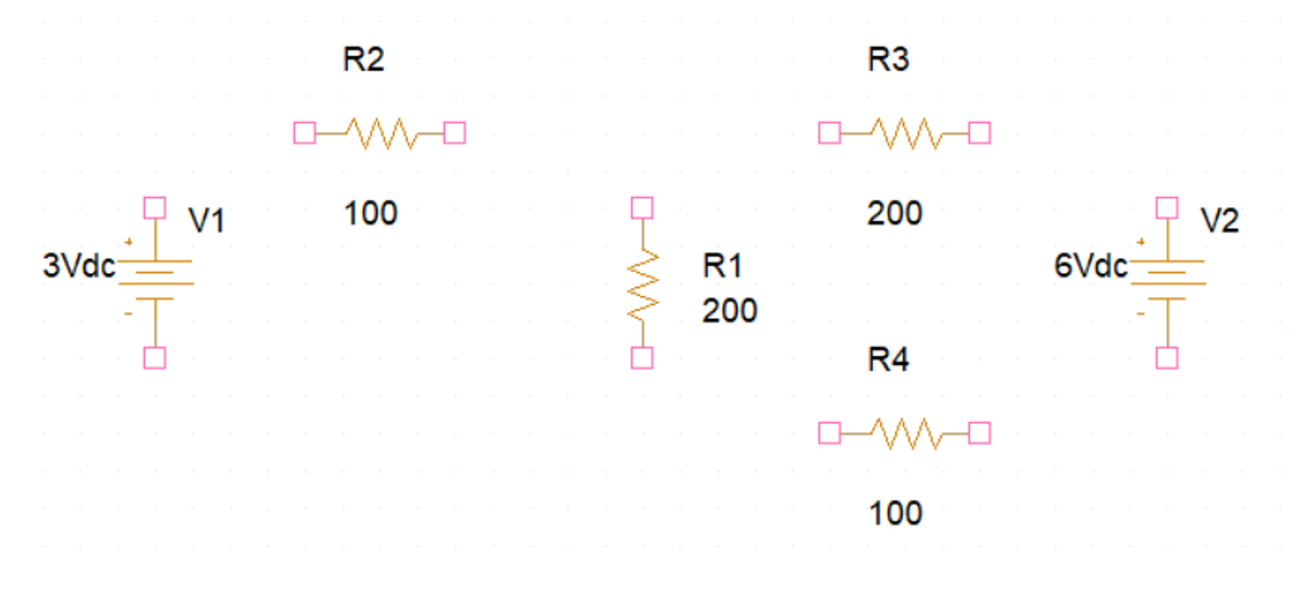
\includegraphics[width=4in]{source/picture/bai_1/pic9.PNG}
    \caption{\textit{Place the power supply using VDC component}}
    \label{bai1_pic9}
\end{figure}

\textbf{Step 4: } Wire all components by selecting the Wire command on the right panel (hot key is W).

\begin{figure}[!htp]
    \centering
    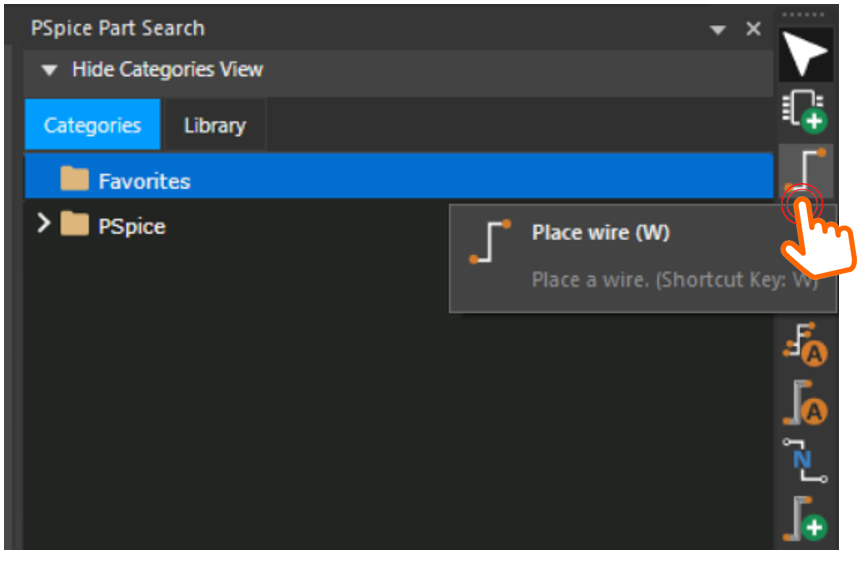
\includegraphics[width=4in]{source/picture/bai_1/pic10.PNG}
    \caption{\textit{Wire the whole circuit}}
    \label{bai1_pic10}
\end{figure}

By clicking a start point and an end point, a wire is placed. In order to delete, select the wire and press \textbf{Delete}. The picture of the circuit after this step is depicted as follow.
\newpage
\begin{figure}[!htp]
    \centering
    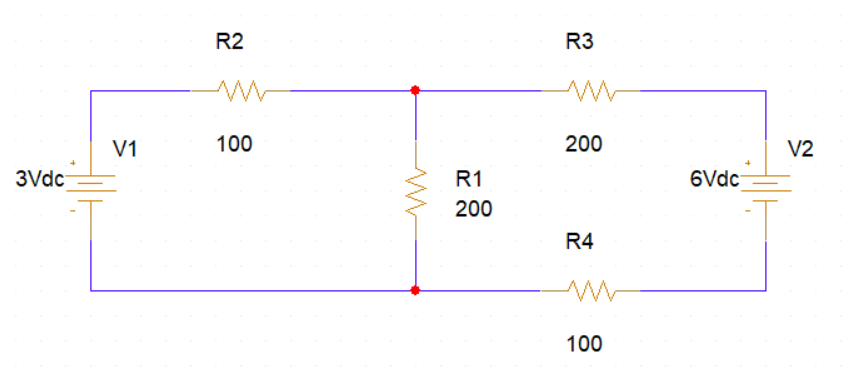
\includegraphics[width=4in]{source/picture/bai_1/pic12.PNG}
    \caption{\textit{Finish all wire in the circuit}}
    \label{bai1_pic12}
\end{figure}

\textbf{Step 5: } Place a Ground symbol. This step is very important to analyze the voltage in a circuit as a reference voltage (0V) is required. The ground symbol is available on the right panel of the software.
\begin{figure}[!htp]
    \centering
    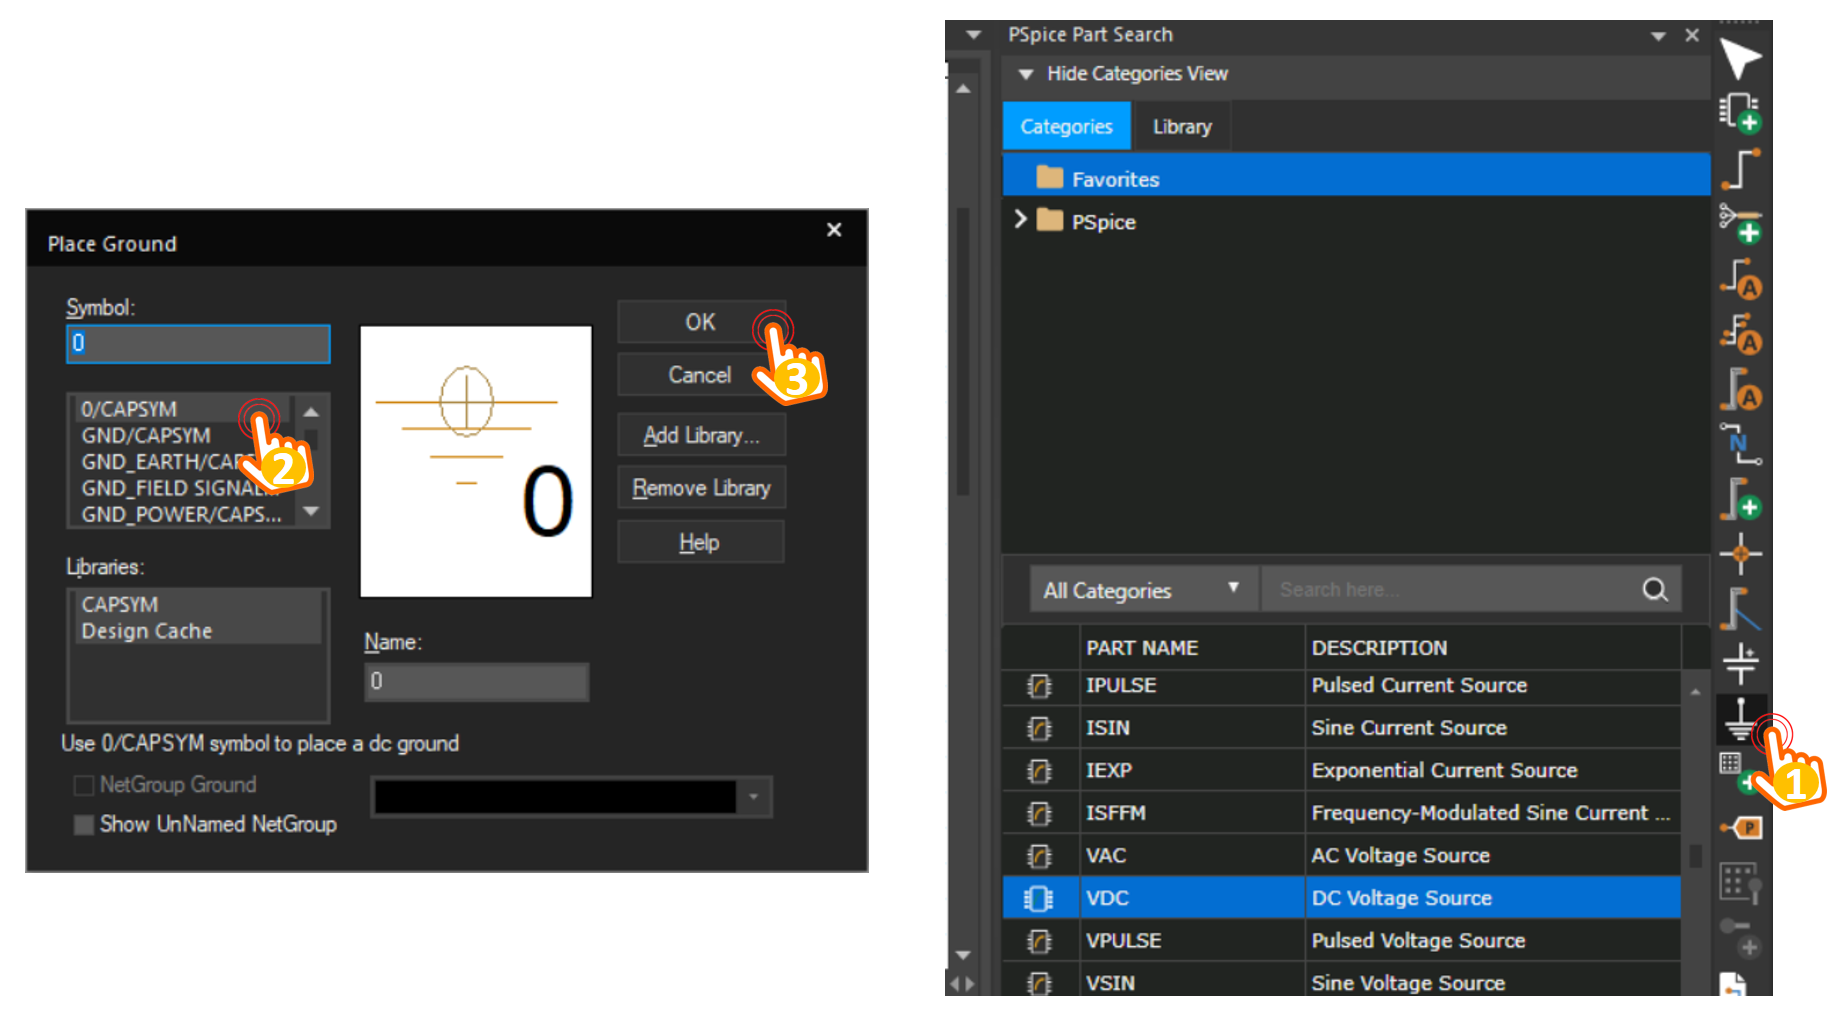
\includegraphics[width=5in]{source/picture/bai_1/pic11.PNG}
    \caption{\textit{Add a ground symbol to the circuit}}
    \label{bai1_pic11}
\end{figure}

Wiring the ground to a point in the circuit, the final result should be like the figure bellow.

\begin{figure}[!htp]
    \centering
    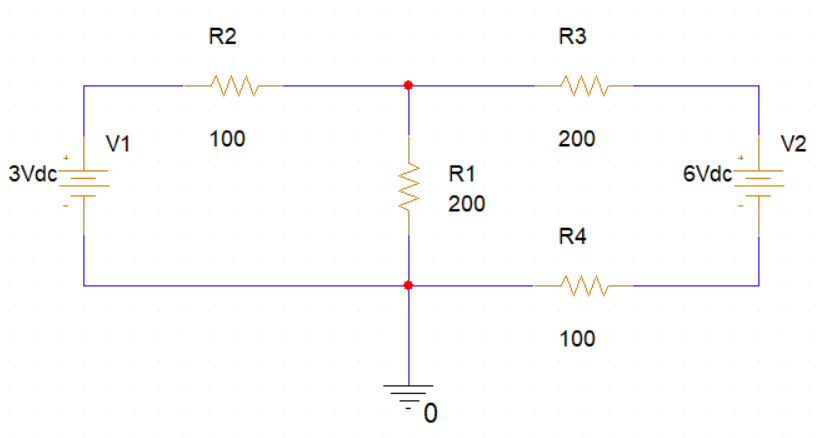
\includegraphics[width=4in]{source/picture/bai_1/pic13.PNG}
    \caption{\textit{A ground point is added to the circuit}}
    \label{bai1_pic13}
\end{figure}

\section{Create a simulation profile}
Before the simulation is started, a simulation profile (or the simulation configuration) is required. From menu \textbf{PSpice}, select \textbf{New Simulation Profile} as follow:
\begin{figure}[!htp]
    \centering
    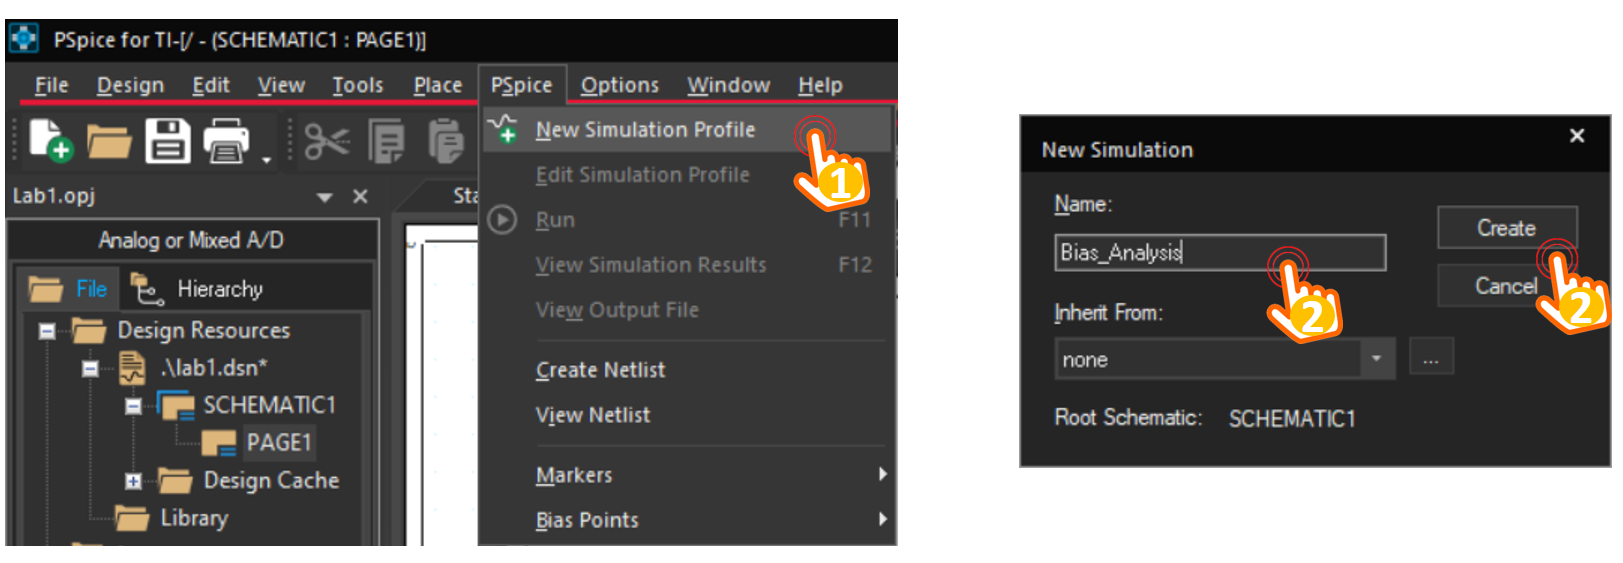
\includegraphics[width=5.5in]{source/picture/bai_1/pic14.PNG}
    \caption{\textit{Create a simulation profile}}
    \label{bai1_pic14}
\end{figure}

When the simulation setting dialog is appeared, please select the \textbf{Bias Point} for analysis type.
\begin{figure}[!htp]
    \centering
    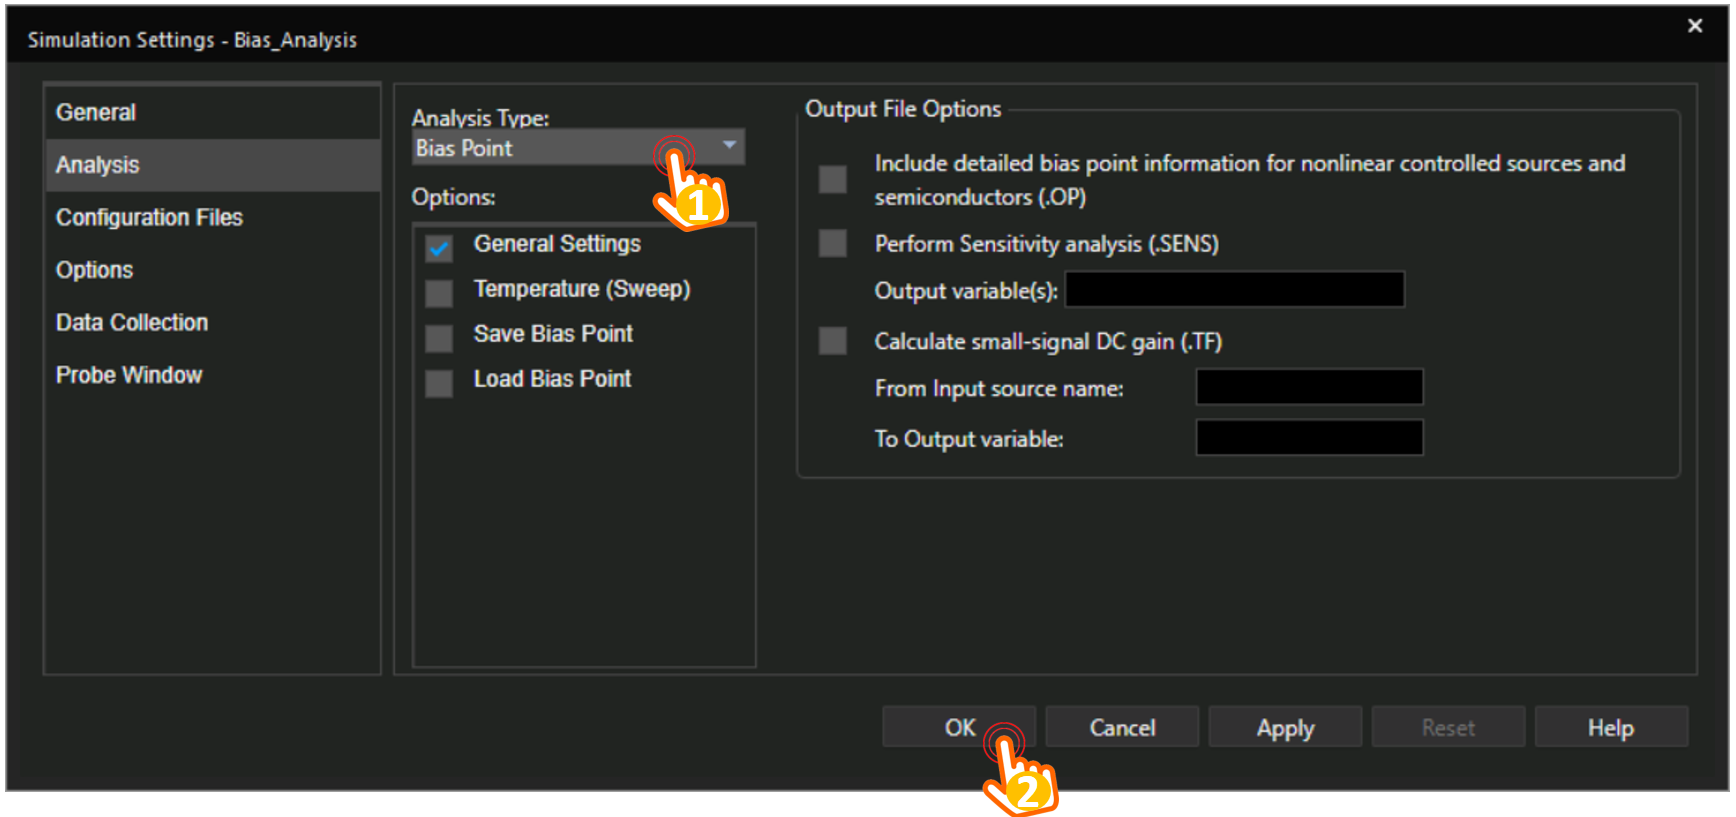
\includegraphics[width=4in]{source/picture/bai_1/pic15.PNG}
    \caption{\textit{Select Bias Point simulation}}
    \label{bai1_pic15}
\end{figure}

In PSpice, the bias point analysis calculates the node voltages and currents through the devices in the circuit. Bias point analysis also takes into account any voltage sources applied to the circuit and any initial conditions set on devices or nodes in the circuit. \\

Finally, click on menu \textbf{PSpice} to select \textbf{Run}, or press \textbf{F11} to start the simulation. The simulation results are displayed directly on the circuit as follow:

\begin{figure}[!htp]
    \centering
    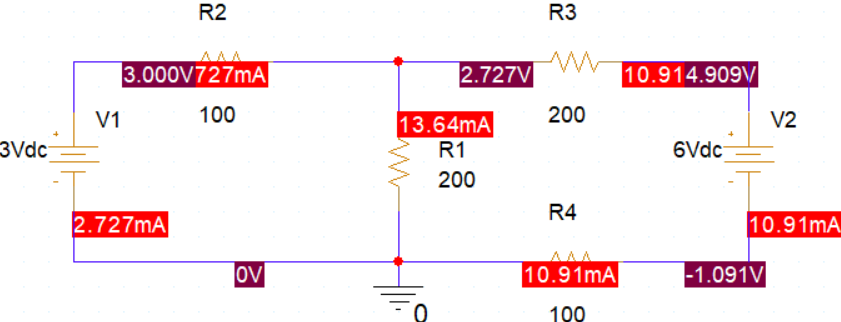
\includegraphics[width=4in]{source/picture/bai_1/pic16.PNG}
    \caption{\textit{Volate and Current in the whole circuit}}
    \label{bai1_pic16}
\end{figure}

In order to display simulation results, go to menu \textbf{PSpice}, select \textbf{Bias Point} and enable the information you need. Students are also proposed to double check their solutions with the simulation results.

\def\answer{1}
\section{Exercise and Report}
In this section, students are proposed to work in some circuit analysis, mostly based on resistors. Some explanations are required and will be considered as a part of the report. Note that the calculation subsection expects to see formulas and equations rather than only the results.

\subsection{Exercise 1}
Given the following circuit. Calculate the value of the voltage $v_0$ and the current $i$. Then, simulate the circuit to check it out.

\begin{figure}[!htp]
    \centering
    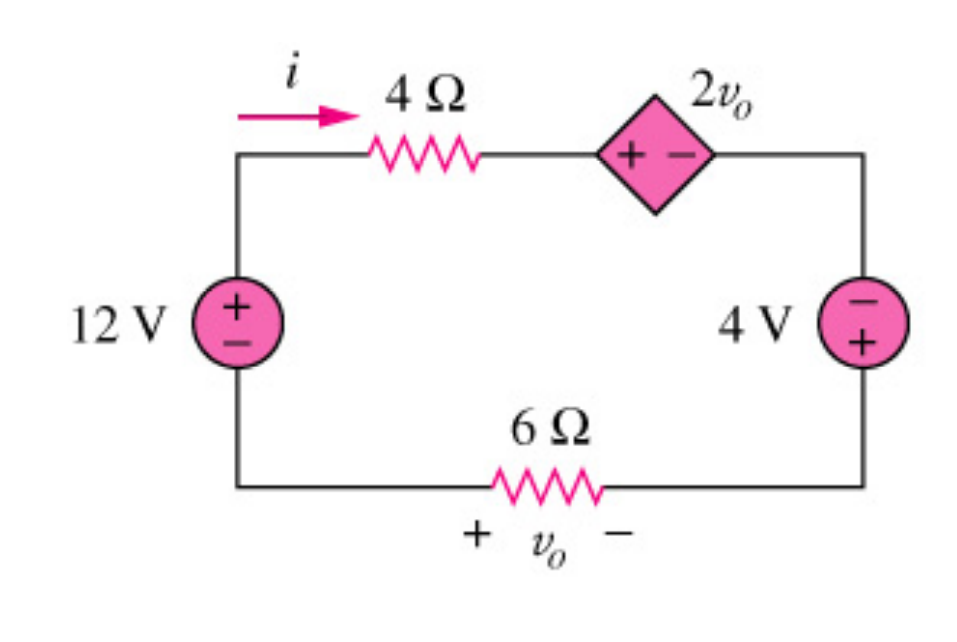
\includegraphics[width = 7cm]{source/picture/bai_1/Bai1_de.png}
    \caption{Find the voltage and the current in the given circuit using KVL}
    \label{lab1_ex1_de}
\end{figure}

\subsubsection{Calculation}
\textit{\textbf{Notes:}}\\
\textit{Explanations, formulas, and equations are expected rather than only results.}\\

According to the:  Kirchoff Voltage Law (KVL)\bigskip\\
We have the first equation:  \dotfill $-4i+2v_0-4-v_0-12=0$ \dotfill\bigskip(1)\\
According to the:  Ohm's Law\bigskip\\
We have the second equation: \dotfill $v_0 = 6i$\dotfill\bigskip(2)\\
From (1) and (2) we have:\bigskip\\
$v_0 = 48$ \dotfill\bigskip\\
$i = 8$ \dotfill\bigskip\\

\subsubsection{Simulation}

\textbf{\textit{Tips:}}\\
To get the Voltage Controlled Voltage Source (VCVS) from the PSpice, under the \textit{\textbf{Place}} menu, find \textbf{\textit{PSpice Component > Source > Controlled Sources > VCVS}}.

A circuit used for the simulation in this exercise maybe like this:
\begin{figure}[H]
    \centering
    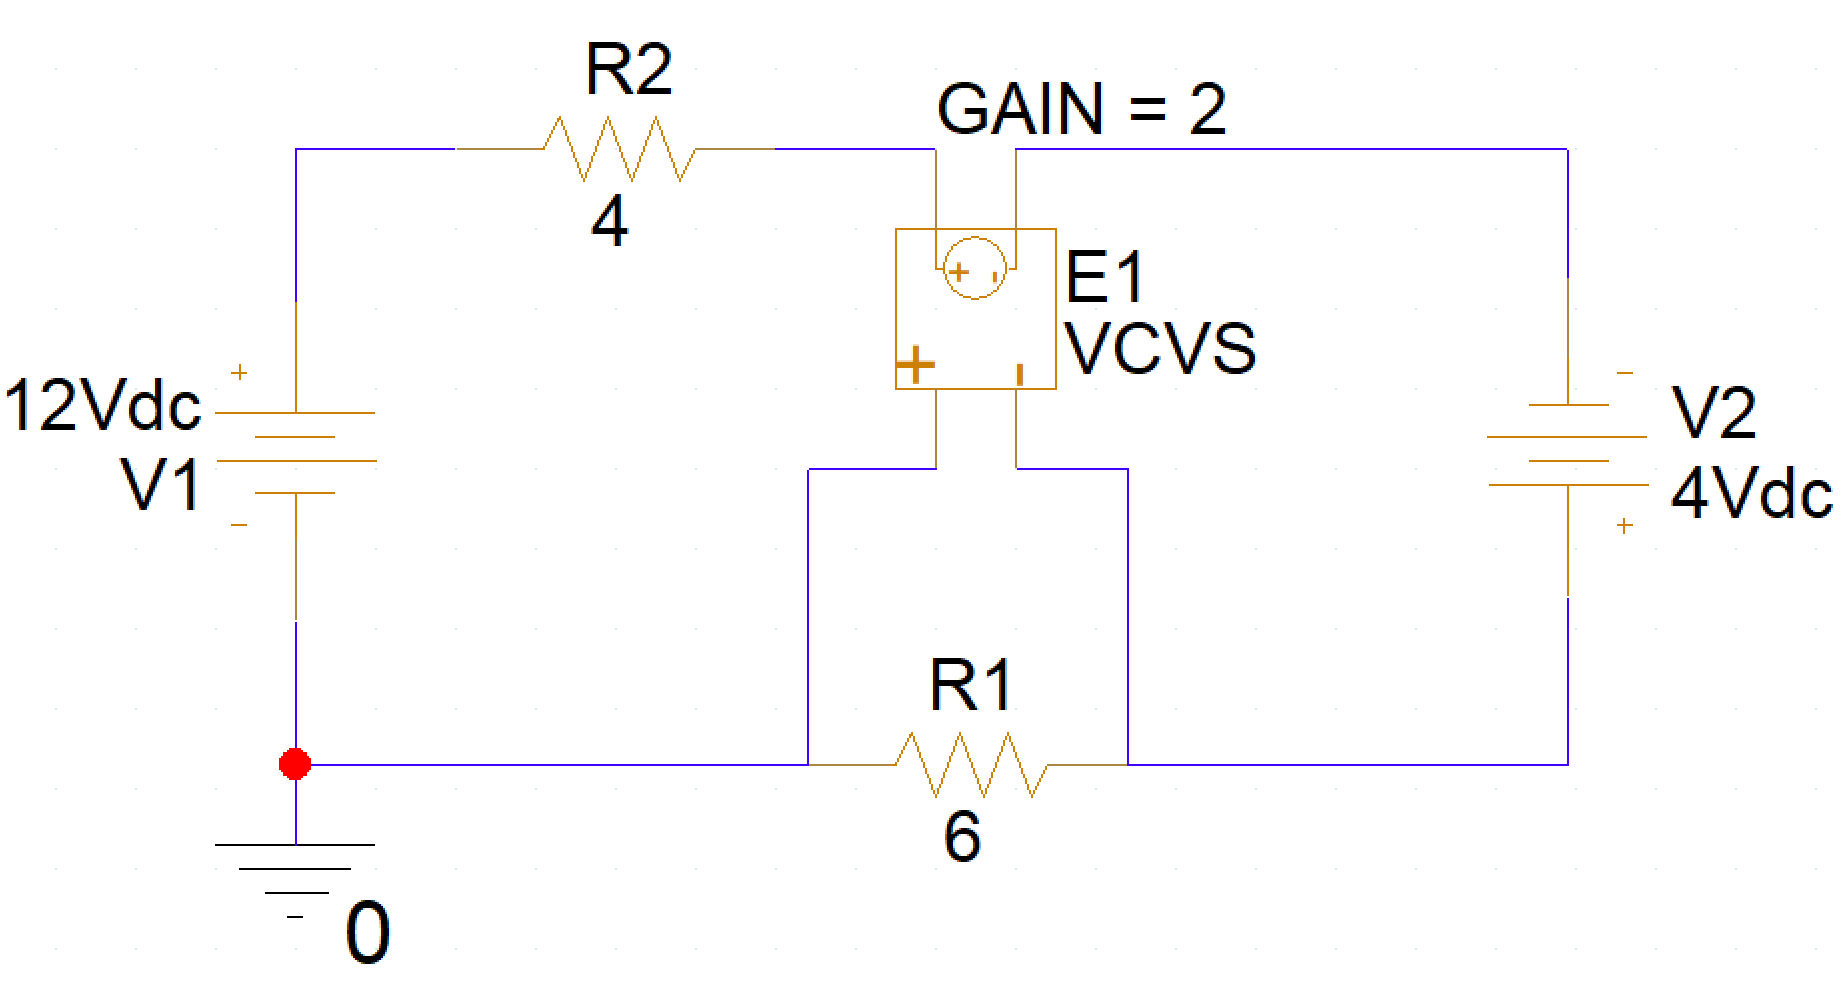
\includegraphics[width = 10cm]{source/picture/bai_1/Bai1_ps.png}
    \caption{A circuit containing a Voltage Controlled Voltage Source in PSpice}
\end{figure}

\textit{\textbf{Simulation result (image):}}
\begin{figure}[H]
    \centering
    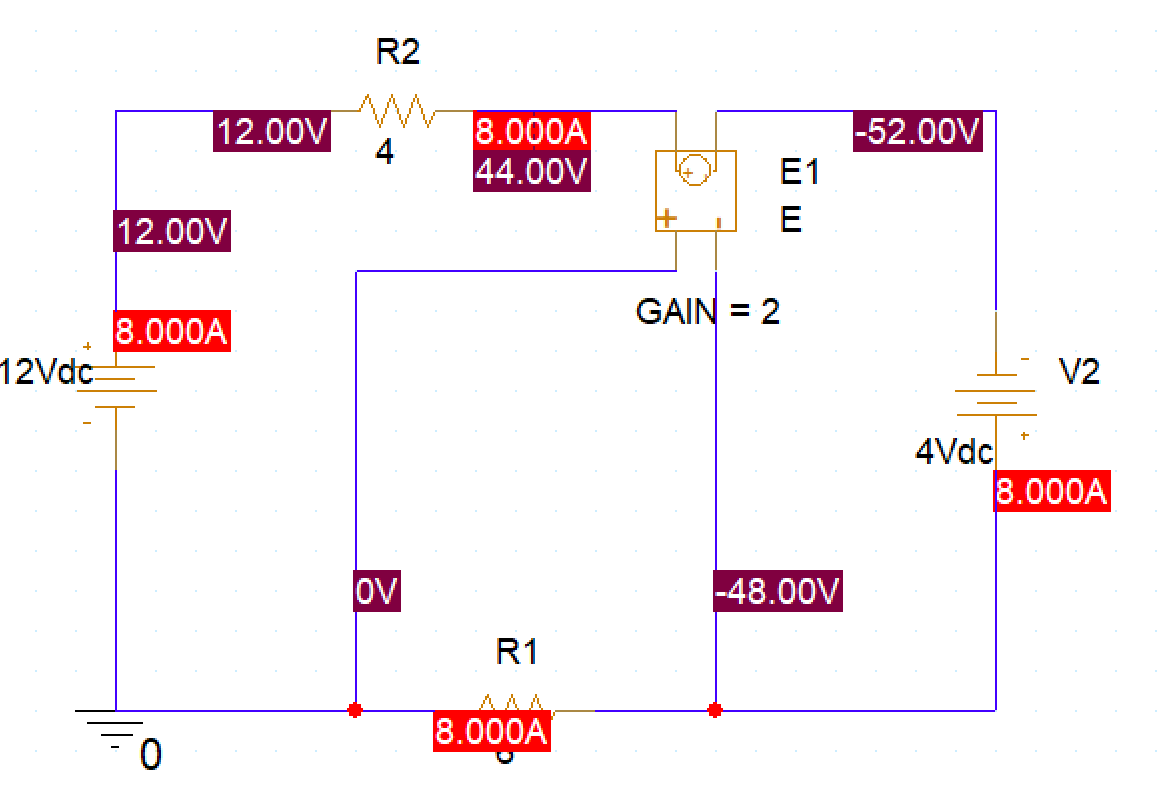
\includegraphics[width = 10cm]{source/picture/bai_1/ex1.png}
\end{figure}
\newpage

\subsection{Exercise 2}
Given the following circuit, students rearrange the circuit to clarify its serial and/or parallel topology. Then, apply the knowledge you've learned to find the equivalent resistance value between two circuit terminals A and F. Finally, perform the simulation to check if the current through the whole circuit is correctly calculated.

\begin{figure}[H]
    \centering
    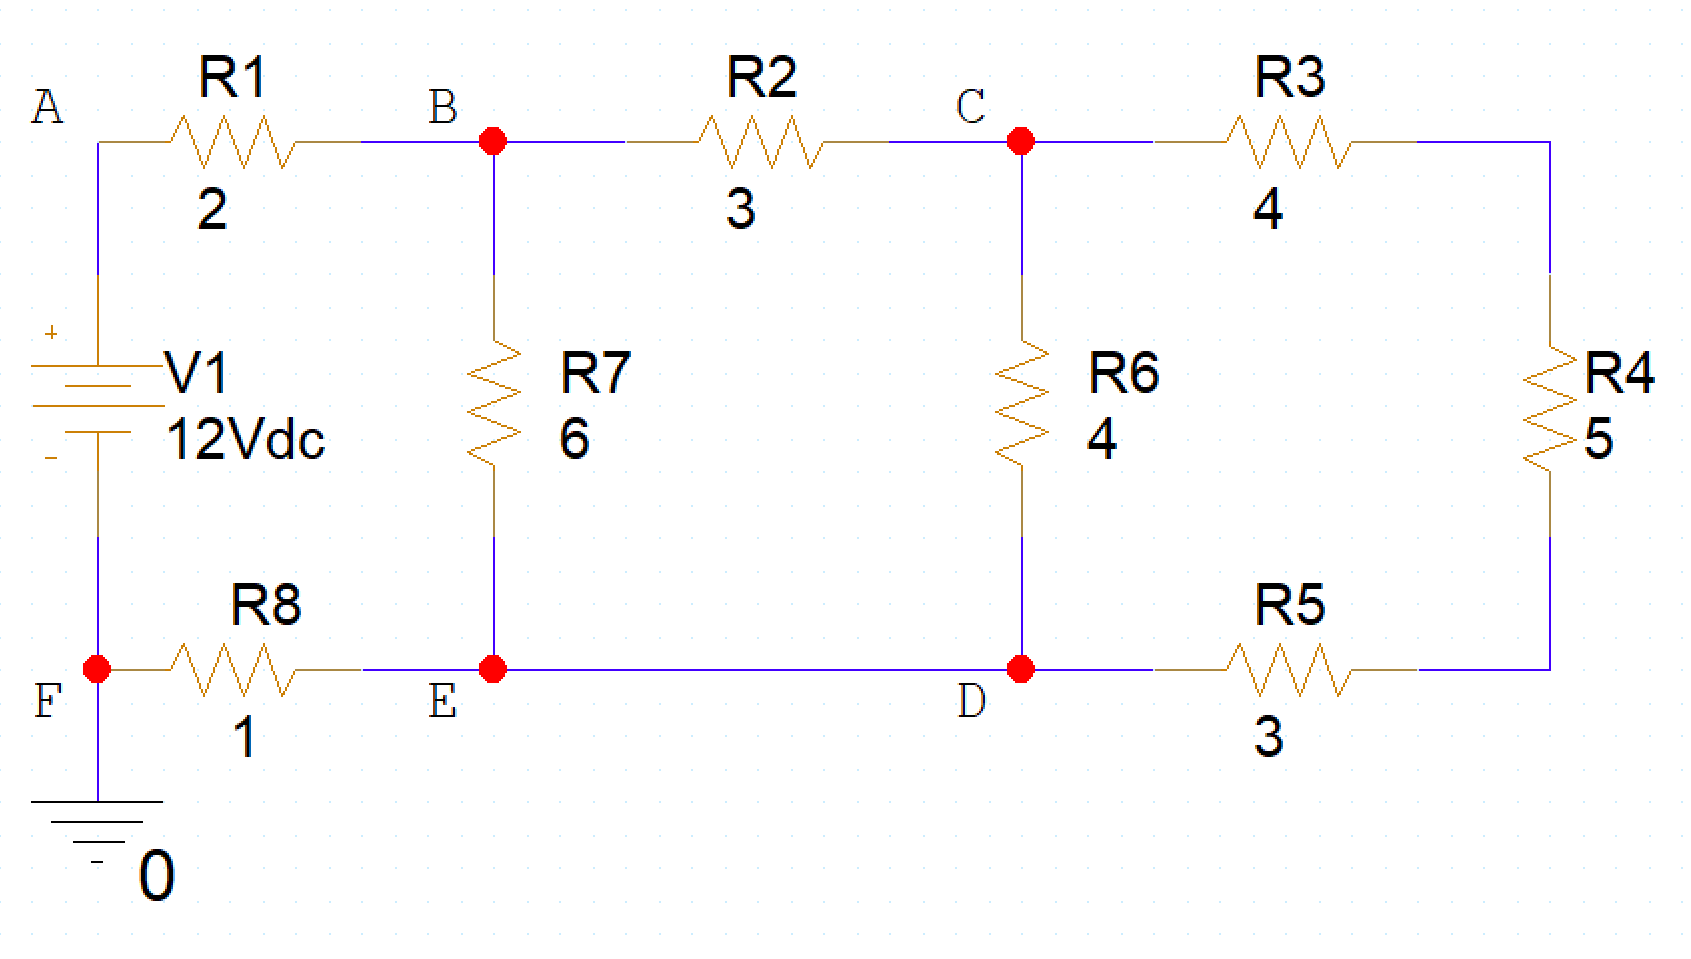
\includegraphics[width = 10cm]{source/picture/bai_1/Bai2_de.png}
    \caption{Find the equivalent resistance value between terminals A and F}
    \label{lab1_ex2_de}
\end{figure}

\subsubsection{Rearrange the circuit}
\textit{Insert the rearranged circuit here. Don't forget the resistance values and the nodes' names.}
\begin{figure}[H]
    \centering
    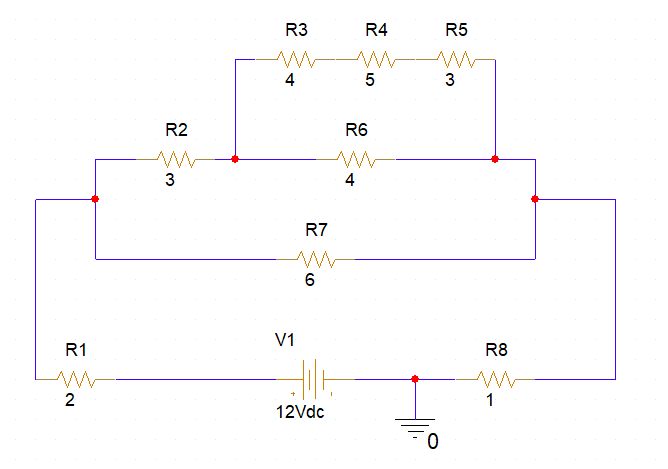
\includegraphics[width = 10cm]{source/picture/bai_1/ex2.png}
    \label{lab1_ex2}
\end{figure}
\newpage

\subsubsection{Calculation}
\textit{\textbf{Convention:}}\\
\textit{The equivalent resistance between the two terminals A and B of a circuit segment containing only R1, R2, R3, and R4 may be named $R_{AB\_1234}$.}\\
\\
\textit{\textbf{Notes:}}\\
\textit{Explanations, formulas, and equations are expected rather than only results.}\\
\\
$R_{CD\_3456} = \frac{R_6(R_3+R_4+R_5)}{R_3+R_4+R_5+R_6}=3\Omega$  as $R_6$ // $R_{345}$\bigskip\\
$R_{BE} = (\frac{1}{R_{CD}+R_2}+\frac{1}{R_7})^{-1}= \frac{1}{6} +\frac{1}{3+3}=3\Omega$ as $R_{CD},R_2$ // $R_7$\bigskip\\
$R_{AF} = R_{BE} + R_1 + R_8 = 3+2+1=6\Omega$\bigskip\\
$I_{AB} = I = \frac{U}{R_{eq}} = \frac{U}{R_{AF}} = \frac{12}{6} = 2A$ Ohm's Law\bigskip\\

\subsubsection{Simulation}
\textit{\textbf{Simulation result (image):}}
\begin{figure}[H]
    \centering
    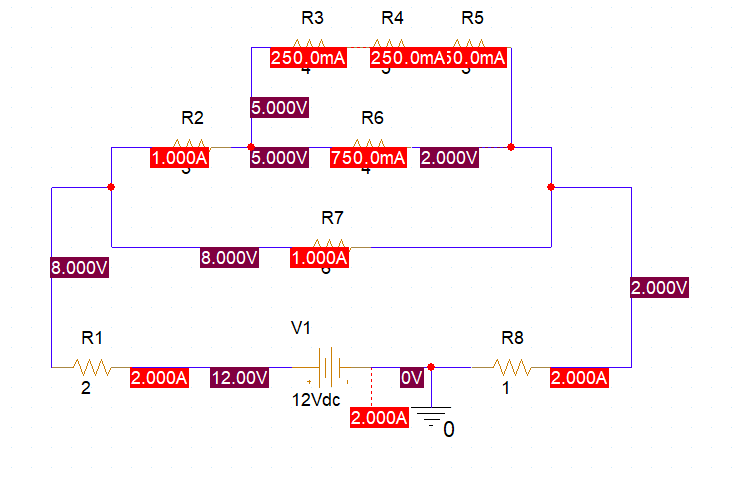
\includegraphics[width = 10cm]{source/picture/bai_1/ex2_sim.png}
\end{figure}
\newpage

\subsection{Exercise 3}
Given the following circuit, students rearrange the circuit to clarify its serial and/or parallel topology. Next, apply the knowledge you've learned to find the equivalent resistance value between two circuit terminals A and F, the voltage values at A, B, C, D, and E. Finally, perform the simulation to check your calculation.

\begin{figure}[H]
    \centering
    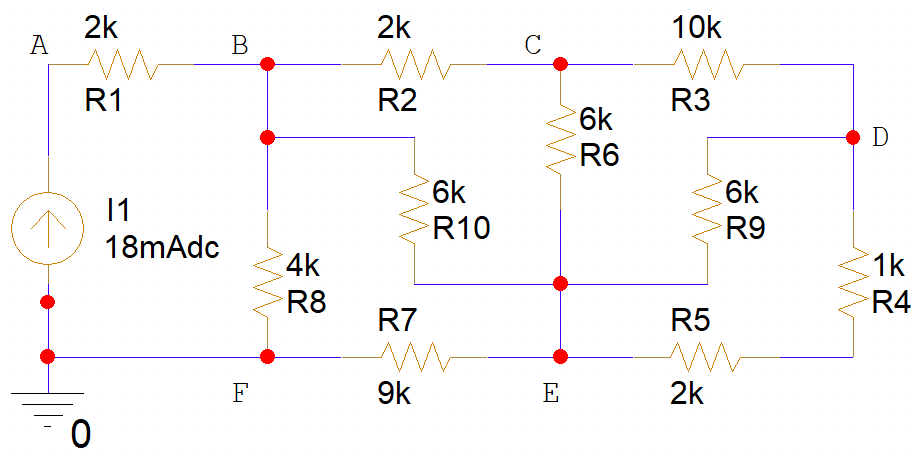
\includegraphics[width = 11cm]{source/picture/bai_1/LAB1_EX3_de.png}
    \caption{Find the whole-circuit equivalent resistance and the voltages at A, B, C, D, and E}
    \label{lab1_ex3_de}
\end{figure}

\subsubsection{Rearrange the circuit}
\textit{Insert the rearranged circuit here. Don't forget the resistance values and the nodes' names.}
\begin{figure}[H]
    \centering
    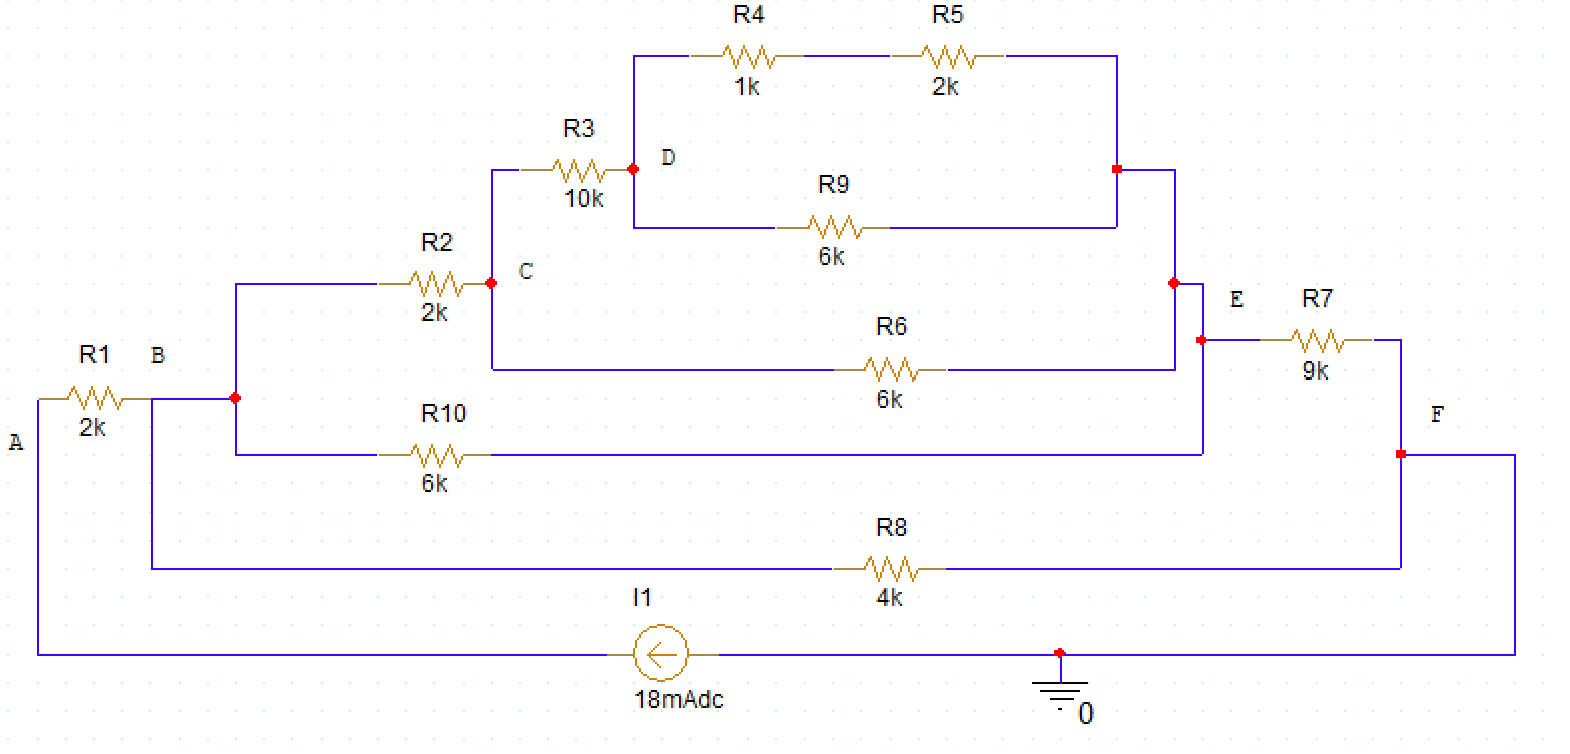
\includegraphics[width = 10cm]{source/picture/bai_1/ex3_rearrange.png}
\end{figure}
\newpage

\subsubsection{Calculation}
\textit{\textbf{Notes:}}\\
\textit{Explanations, formulas, and equations are expected rather than only results.}\\
\\
$$R_{CE} = \left(\frac{1}{R_6}+\frac{1}{R_3 + \frac{R_9(R_4+R_5)}{R_9+R_4+R_5}}\right)^{-1} = \left(\frac{1}{6}+\frac{1}{10 + \frac{6(1+2)}{6+1+2}}\right)^{-1} = 4(k\Omega)$$
$$R_{BE} = \left(\frac{1}{R_10} + \frac{1}{R_2 + R_{CE}}\right)^{-1} = \left(\frac{1}{6}+\frac{1}{2+4}\right)^{-1} = 3(k\Omega)$$
$R_{AF} =R_1 + \frac{R_8(R_{BE}+R_7)}{R_8 + R_{BE} + R_7} = 2 + \frac{4(3+9)}{4+3+9} = 5(k\Omega)$ \bigskip\\
$V_A = I_1 \times R_{AF} = 18 \times 5 = 90 $ \bigskip\\
$V_B = V_A - R_1 \times I_1 = 90 -2 \times 18 = 54$ \bigskip\\
$V_C = V_B - \left(\frac{V_B-V_E}{R_{BE}} - \frac{V_B-V_E}{R_{10}}\right) \times R_2 = 54 - \left(\frac{54-40.5}{3} - \frac{54-40.5}{6}\right) \times 2 = 49.5 (V)$ \bigskip\\
$V_D = V_C - \left(\frac{V_C-V_E}{R_{CE}} - \frac{V_C-V_E}{R_{6}}\right) \times R_3 = 49.5 - \left(\frac{49.5-40.5}{4} - \frac{49.5-40.5}{6}\right) \times  10= 42 (V)$ \bigskip\\
$V_E = V_F + \left(\frac{V_A}{R_{BF}} - \frac{V_A}{R_8}\right) \times 9 = 0 + \left(\frac{54}{3} - \frac{54}{4}\right) \times 9 = 40.5 (V)$ \bigskip\\

\subsubsection{Simulation}
\textit{\textbf{Simulation result (image):}}
\begin{figure}[H]
    \centering
    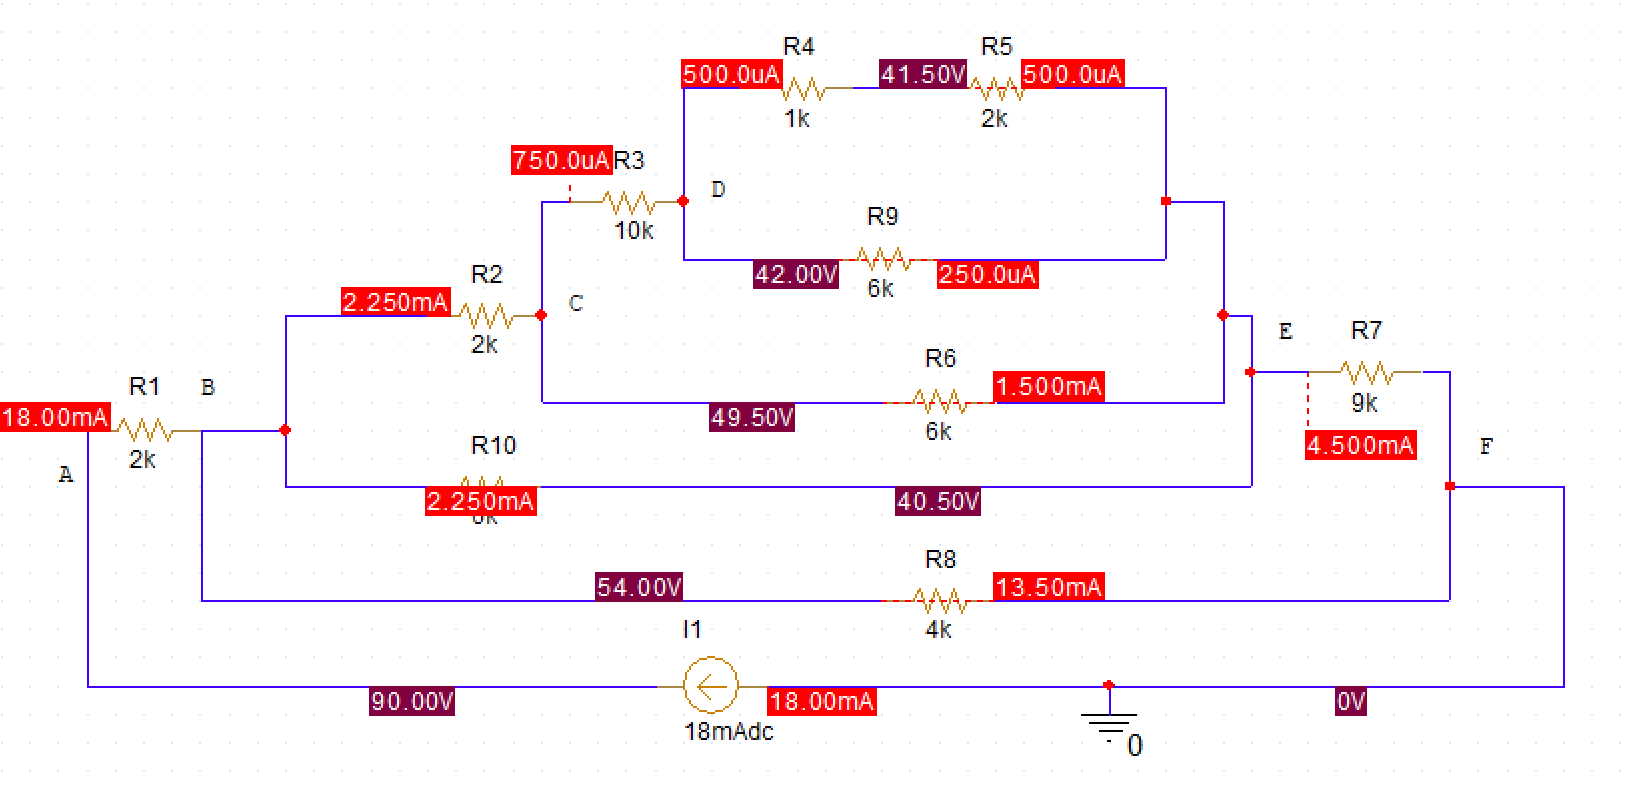
\includegraphics[width = 10cm]{source/picture/bai_1/ex3_sim.png}
\end{figure}
\newpage

\subsection{Exercise 4}
Given the following circuit, find $I_1$, $I_2$, $I_3$, $V_a$, and $V_b$. Present your calculation steps and check them out by performing the simulation.

\begin{figure}[H]
    \centering
    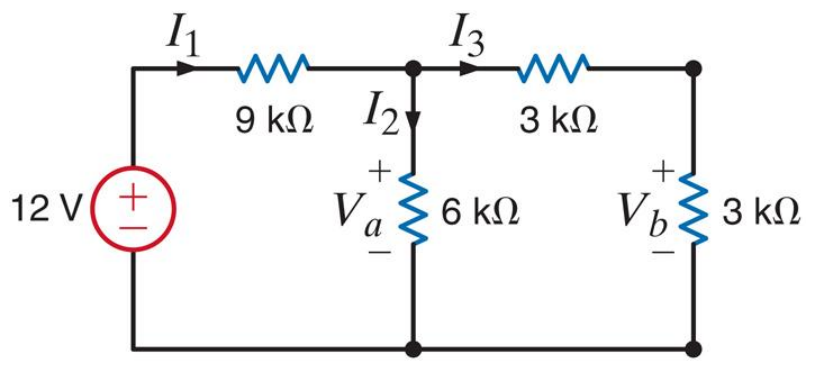
\includegraphics[width = 8cm]{source/picture/bai_1/lab1_ex4_de.png}
    \caption{Find $I_1$, $I_2$, $I_3$, $V_a$, and $V_b$}
    \label{lab1_ex4_de}
\end{figure}

\subsubsection{Calculation}
\textit{\textbf{Notes:}}\\
\textit{Explanations, formulas, and equations are expected rather than only results.}\\
\\ \\
Equivalent Resistor:
$$ R_{eq} = R_1 + \left(\frac{1}{R_2 + R_3} + \frac{1}{R_4} \right)^{-1} = 9 + \frac{(3+3)6}{3 + 3 + 6} = 12(k\Omega) $$

Using KCL: $I_1 = I_2 + I_3$\\
Using KVL:
$\begin{cases}
        -12 + 9I_1 + 6I_2 = 0 \\
        -6I_2 + 3I_3 + 3I_3 = 0
    \end{cases}$ \\
Solving the system of three aforementioned equations:
$\begin{cases}
        I_1 = 1 (mA)  \\
        I_2 = 0.5(mA) \\
        I_3 = 0.5(mA)
    \end{cases}$
\\
$V_a = 6 \times I_2 = 6 \times 0.5 = 3 (V)$ \\
$V_b = 3 \times I_3 = 3 \times 0.5 = 1.5(V)$ \\


\subsubsection{Simulation}
\textit{\textbf{Simulation result (image):}}
\begin{figure}[H]
    \centering
    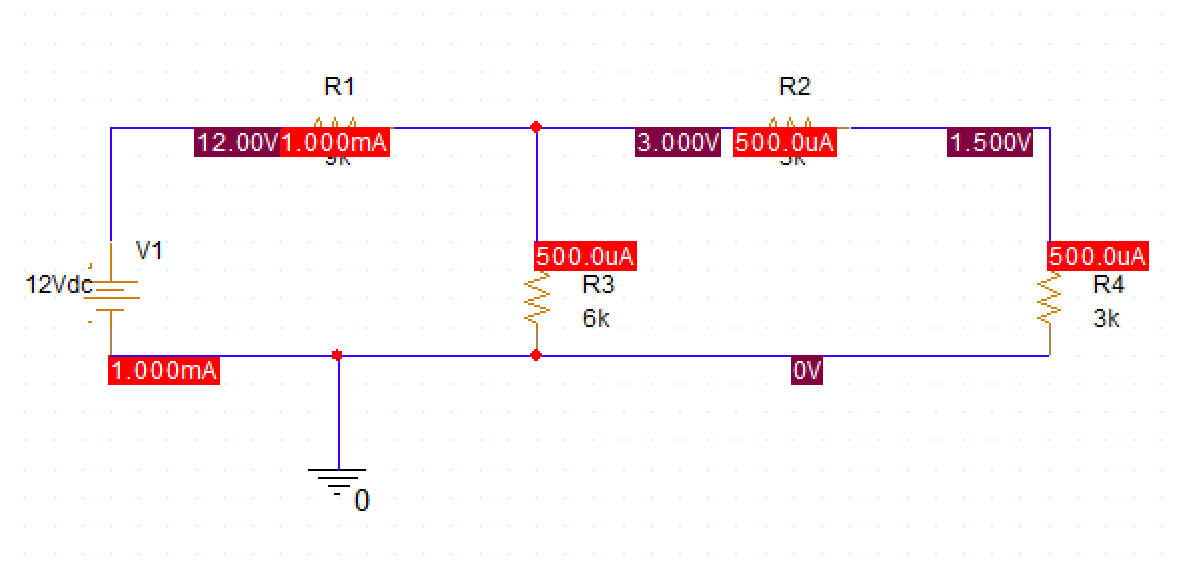
\includegraphics[width = 10cm]{source/picture/bai_1/ex4_sim.png}
\end{figure}
\newpage

\subsection{Exercise 5}
Given the network as shown below:

\begin{figure}[H]
    \centering
    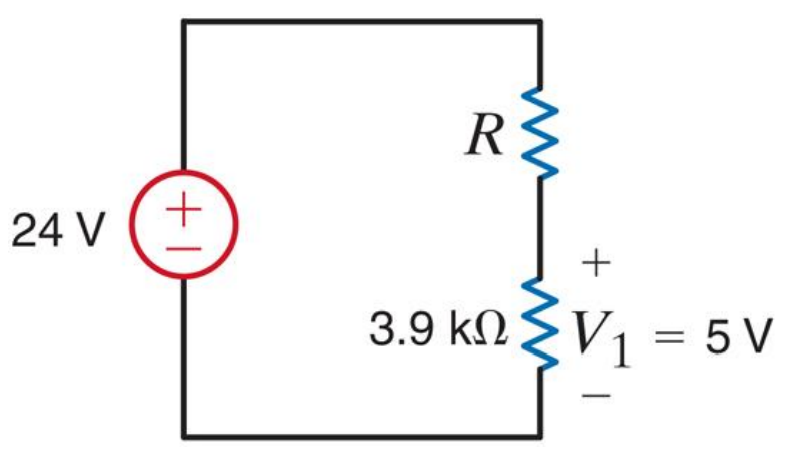
\includegraphics[width = 6cm]{source/picture/bai_1/lab1_ex5_de.png}
    \caption{Select resistor R from the standard resistors list and do the following requirement}
    \label{lab1_ex5_de}
\end{figure}

\textit{\textbf{Notes:}}\\
\textit{Explanations, formulas, and equations are expected rather than only results.}\\

\begin{enumerate}[label=\alph*.]
    \item Find the required value for the resistor R.\bigskip\\
          $R = 14.82 (k\Omega)$ as $3.9 \frac{24}{3.9+x} = 5$\medskip
    \item Use Table 2.1 in the lecture slide to select a standard 10\% tolerance resistor for R. R in the circuit may be a single resistor or a combination of many resistors as long as these resistors are meet the standard values and are available in the market.\bigskip\\
          \\
          The selected resistor: $R = 15 (k\Omega) \pm 10\%$\bigskip
    \item Using the resistor selected in (b), determine the voltage across the 3.9k resistor.\bigskip\\
          The value of $V_1$ according to the selected resistor R:$3.9 \times \frac{24}{3.9 + 15} = 4.9524 (k\Omega)$\medskip
    \item Calculate the percent error in the voltage V1, if the standard resistor selected in (b) is used.\\
          $$\frac{V_{1'}^{2}}{R} = \frac{4,9524^2}{3.9} = 5,28879 $$
    \item Determine the power rating for this standard component.\bigskip\\
          $P_R = RI^2 = 15 \times \left(\frac{24}{3.9+15}\right)^2 = 24.1875 (mW)$\dotfill\
\end{enumerate}

\subsubsection{Simulation}
\textit{\textbf{Simulation result (image):}}
\begin{figure}[H]
    \centering
    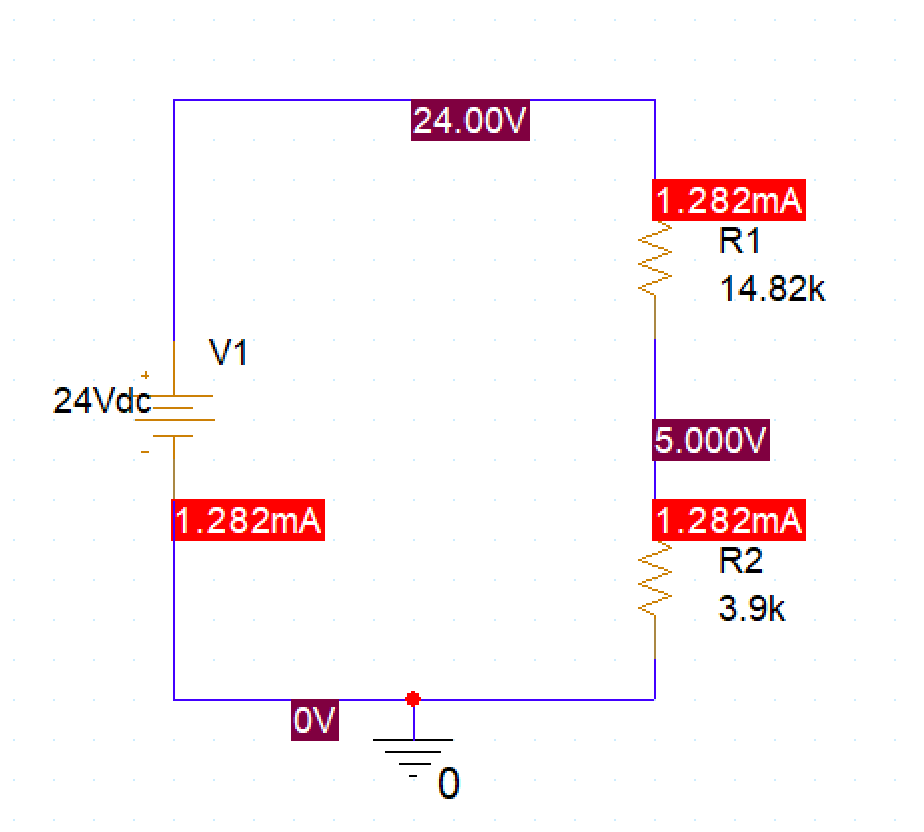
\includegraphics[width = 10cm]{source/picture/bai_1/ex5_sim.png}
\end{figure}

\newpage

\subsection{Exercise 6}
Given the following circuit. Apply the knowledge you've learned to transform it into another form in which you can find total equivalent resistance $R_{ab}$ more easily. Next, find the value of the current $i$ through the circuit and perform a simulation to check it out.

\begin{figure}[H]
    \centering
    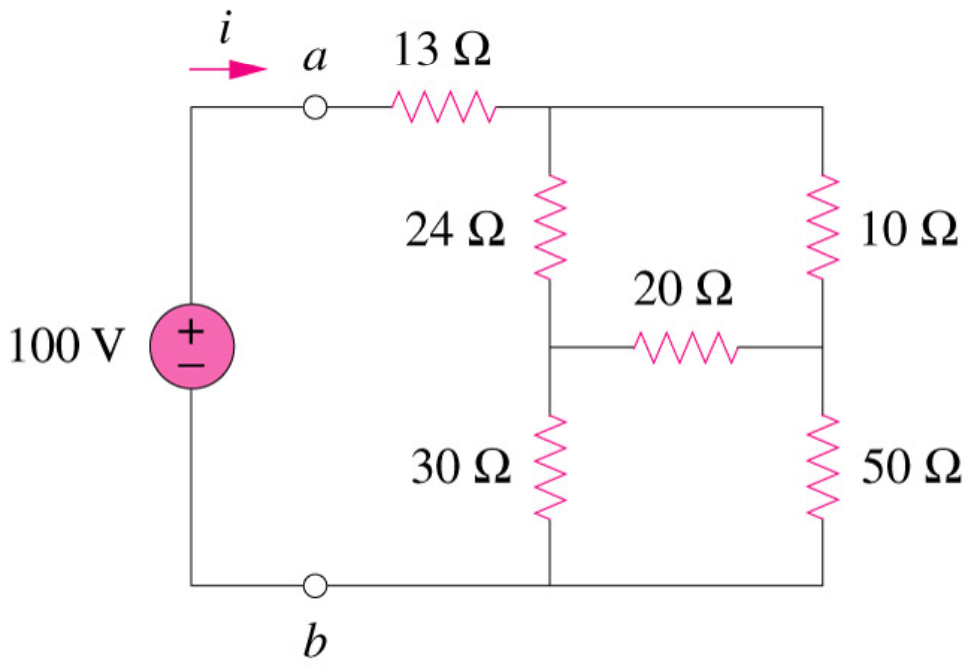
\includegraphics[width = 9cm]{source/picture/bai_1/lab1_ex6_de.png}
    \caption{Transform the circuit, then find the equivalent resistance $R_{ab}$ and the current $i$ through the circuit.}
    \label{lab1_ex6_de}
\end{figure}

\subsubsection{Circuit transformation}
\textit{Insert the transformed circuit here.}
\begin{figure}[H]
    \centering
    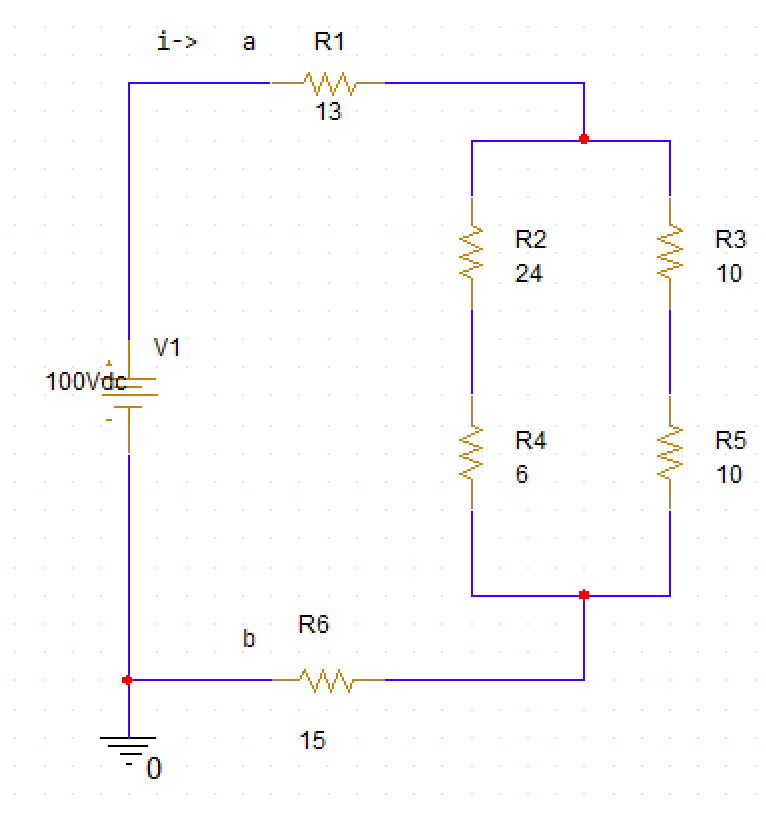
\includegraphics[width = 10cm]{source/picture/bai_1/ex6_rearrange.png}
\end{figure}
\newpage
\textit{Explain any calculations (i.e., write out the formulas you used).}\\
\bigskip
Apply Delta - Wye transformation formular:
$$ R_4 = \frac{R_aR_b}{R_a + R_b + R_c} = \frac{20\cdot 30}{20 + 30 + 50} = 6 (\Omega)$$
$$ R_5 = \frac{R_bR_c}{R_a + R_b + R_c} = \frac{20\cdot 50}{20 + 30 + 50} = 10(\Omega)$$
$$ R_6 = \frac{R_aR_c}{R_a + R_b + R_c} = \frac{30\cdot 50}{20 + 30 + 50} = 15(\Omega)$$
\bigskip


\subsubsection{Calculation}
\textit{\textbf{Notes:}}\\
\textit{Explanations, formulas, and equations are expected rather than only results.}\bigskip\\

$R_2$ and $R_4$ parallel with $R_3$ and $R_5$, in the serial of $R_1$, $R_{2435}$ and $R_6$ \bigskip\\
$R_{ab} = R_1 + \frac{(R_2+R_4)(R_3 + R_5)}{R_2+R_3+R_4+R_5} + R_6= 13 + \frac{(24+6)(10 + 10)}{24+6+10+10} + 15  =  40 (\Omega)$\dotfill\bigskip\\
$i = \frac{V_1}{R_{ab}} = \frac{100}{40} = 2.5 A$\dotfill\bigskip

\subsubsection{Simulation}
\textit{\textbf{Simulation result (image):}}
\begin{figure}[H]
    \centering
    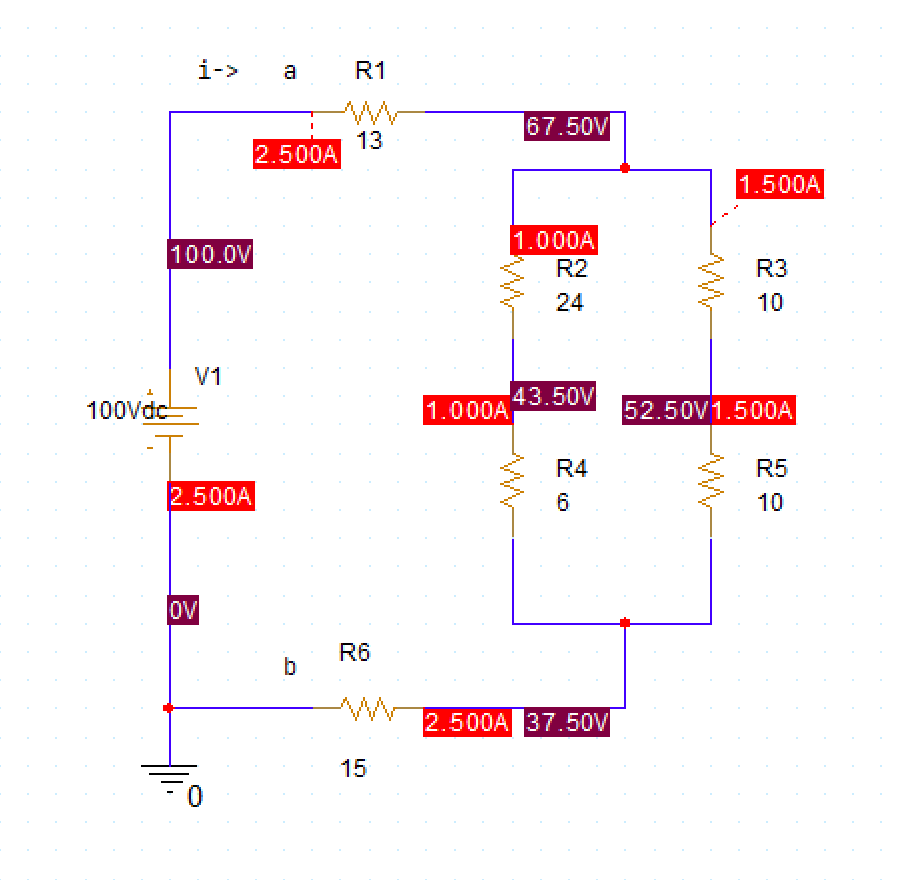
\includegraphics[width = 10cm]{source/picture/bai_1/ex6_sim.png}
\end{figure}
\newpage

\subsection{Exercise 7}
Given the following circuit. Apply the knowledge you've learned to transform it into another form in which you can find total equivalent resistance more easily. Next, find the value of the current $I_S$ through the circuit and perform a simulation to check it out.

\begin{figure}[H]
    \centering
    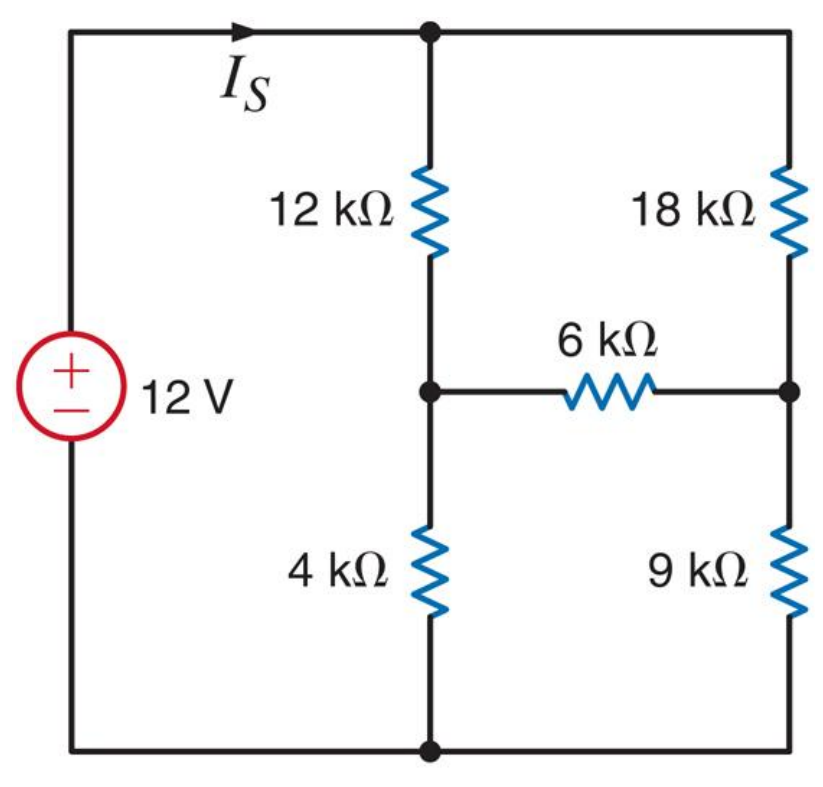
\includegraphics[width = 6cm]{source/picture/bai_1/lab1_ex7_de.png}
    \caption{Transform the circuit, then find the equivalent resistance and the current $I_S$ through the circuit.}
    \label{lab1_ex7_de}
\end{figure}

\subsubsection{Circuit transformation}
\textit{Insert the transformed circuit here.}
\begin{figure}[H]
    \centering
    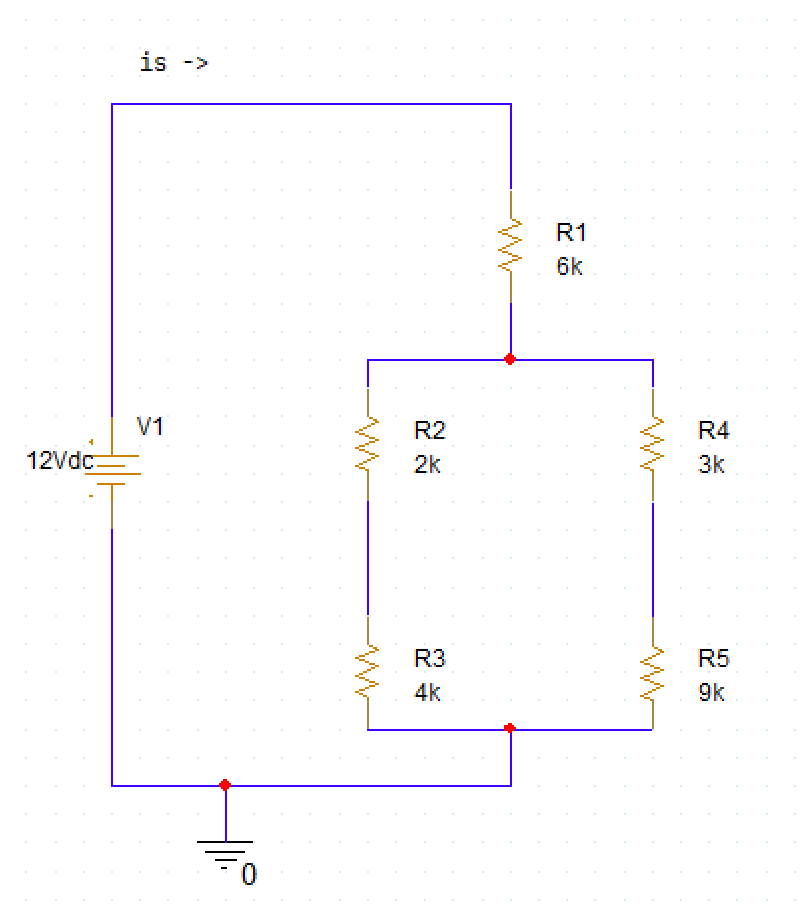
\includegraphics[width = 10cm]{source/picture/bai_1/ex7_rearrange.png}
\end{figure}
\newpage
\textit{Explain any calculations (i.e., write out the formulas you used).}\\
\bigskip
Apply Delta - Wye transformation formular:
$$ R_1 = \frac{R_aR_b}{R_a + R_b + R_c} = \frac{12\cdot 18}{12 + 18 + 6} = 6 (k\Omega)$$
$$ R_2 = \frac{R_bR_c}{R_a + R_b + R_c} = \frac{12\cdot 6}{12 + 18 + 6} = 2 (k\Omega)$$
$$ R_4 = \frac{R_aR_c}{R_a + R_b + R_c} = \frac{6\cdot 18}{12 + 18 + 6} = 3(k\Omega)$$
\bigskip



\subsubsection{Calculation}
\textit{\textbf{Notes:}}\\
\textit{Explanations, formulas, and equations are expected rather than only results.}\bigskip\\

$R_2, R_3$ parallel with $R_4 and R_5$
$R_{equivalent} = 6 + \frac{(2+4)(3+9)}{2+4+3+9} = 10 (k\Omega)$\dotfill\bigskip\\
$I_S = \frac{V_1}{R_{eq}} = \frac{12}{10\times10^{3}} = 1.2 mA$\dotfill\bigskip

\subsubsection{Simulation}
\textit{\textbf{Simulation result (image):}}
\begin{figure}[H]
    \centering
    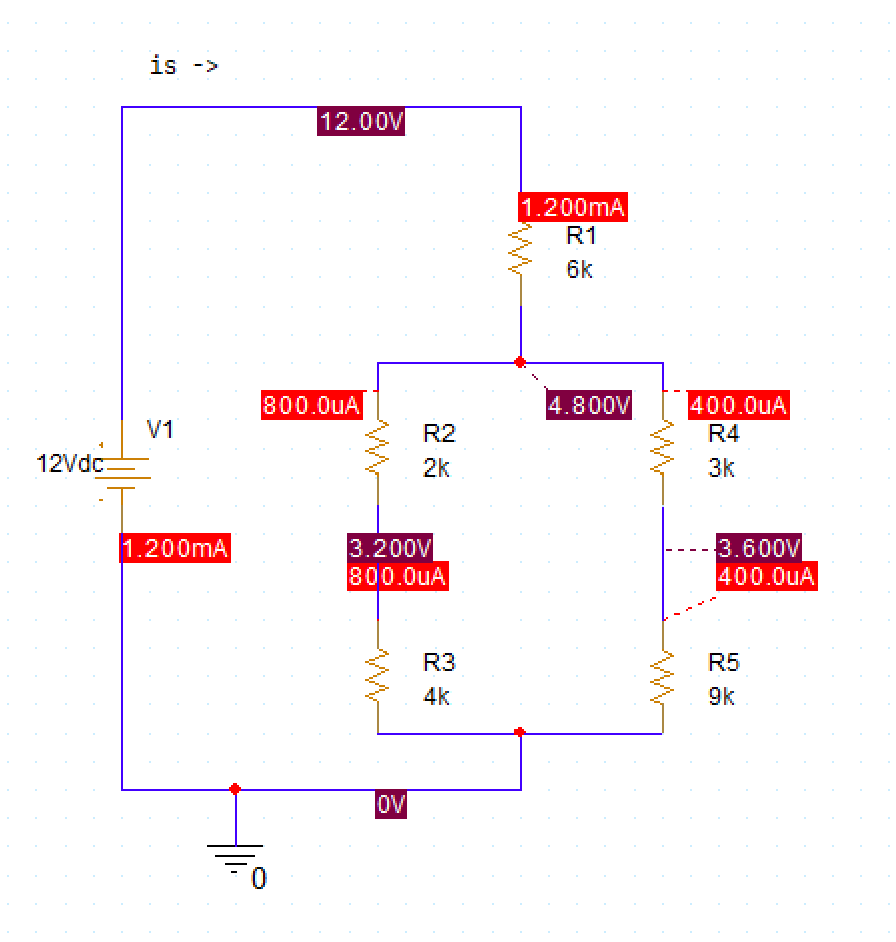
\includegraphics[width = 10cm]{source/picture/bai_1/ex7_sim.png}
\end{figure}
\newpage

\subsection{Exercise 8}
Given the following circuit with $p_2$, $p_3$, and $p_4$ are absorbing powers of unknown electrical elements. First, use the knowledge you've learned to identify whether they are active or passive elements (supplying or absorbing power). To an element absorbing power, use a pure resistor with a proper value as a representative. To a power element, use an ideal DC voltage source with the corresponding value as a representative. Next, redraw the circuit and calculate the power that each element absorbs. Note that here we use the passive sign convention. Then, perform a simulation with the elements determined by the previous step.

\begin{figure}[H]
    \centering
    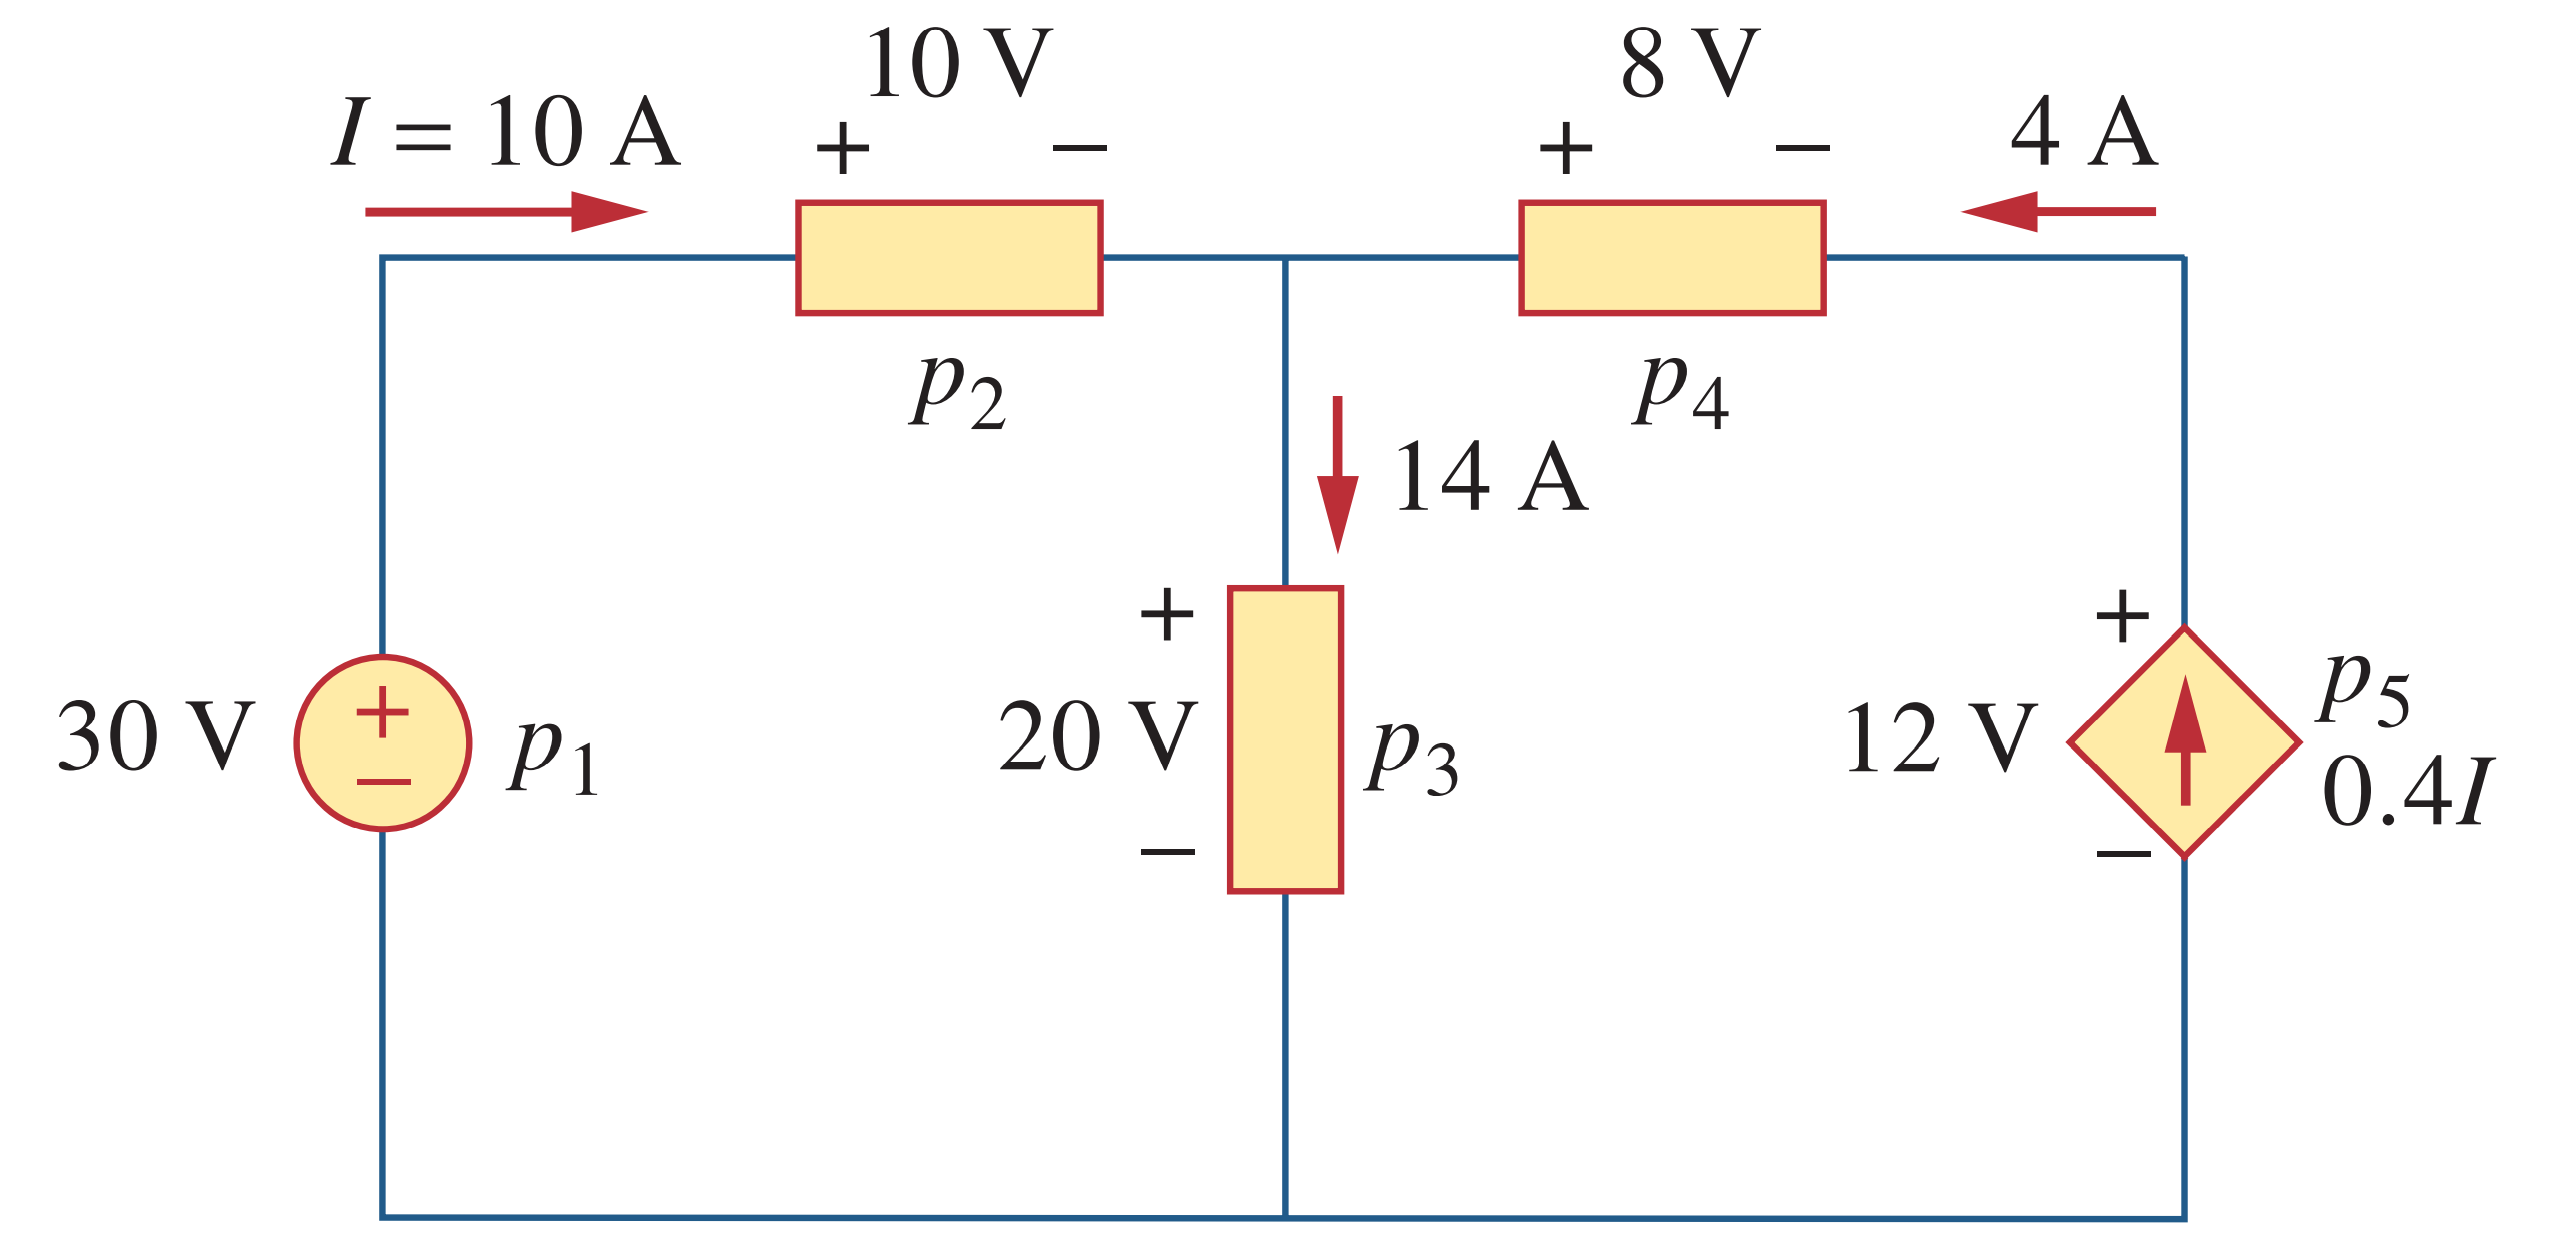
\includegraphics[width =  10cm]{source/picture/bai_1/lab1_ex8_de.png}
    \caption{Determine the unknown elements and calculate the absorbing power of each}
    \label{lab1_ex8_de}
\end{figure}

\subsubsection{Identify the unknown elements}
In Figure \ref{lab1_ex8_de}:\bigskip\\
$p_2 = 10 \times 10 = 100 W$  $\longrightarrow$  passive element\bigskip\\
$p_3 = 14 \times 20 = 280 W$  $\longrightarrow$ passive element\bigskip\\
$p_4 = 4 \times (-12) = -48W$  $\longrightarrow$ active element\bigskip\\

\subsubsection{Redraw the circuit for simulation}
\textit{\textbf{Simulation result (image):}}
\begin{figure}[H]
    \centering
    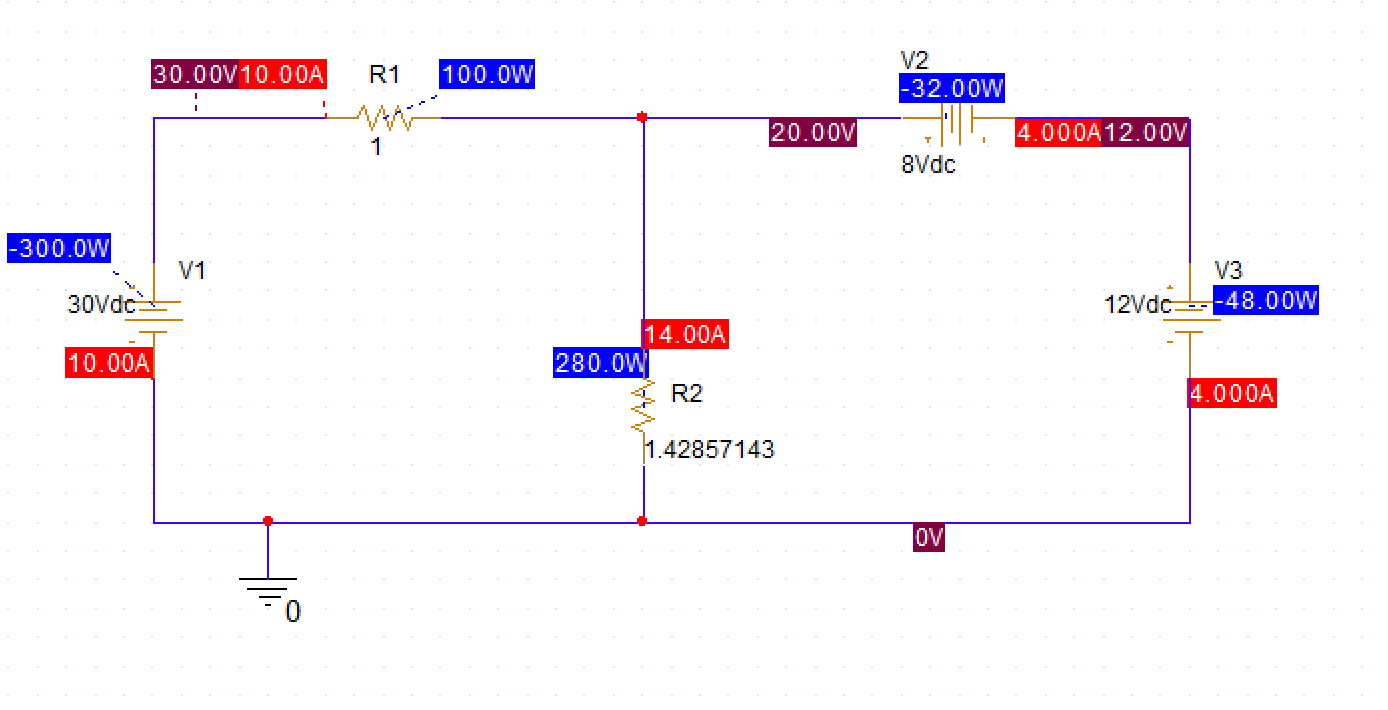
\includegraphics[width = 10cm]{source/picture/bai_1/ex8_sim.png}
    \label{ex8_rearrange}
\end{figure}
\newpage

\subsection{Exercise 9}
Given the following circuit. Find the voltage $v$ and the current $i_x$. According to the result, determine the elements whose absorbing power respectively $p_1$ and $p_2$ are active or passive (calculations are required). Note that here we use the passive sign convention. If an element consumes power, use a pure resistor with an appropriate value as a representative. If it is a  power supply element, use a corresponding ideal DC voltage source to represent it. Perform a simulation to check how the circuit works.

\begin{figure}[H]
    \centering
    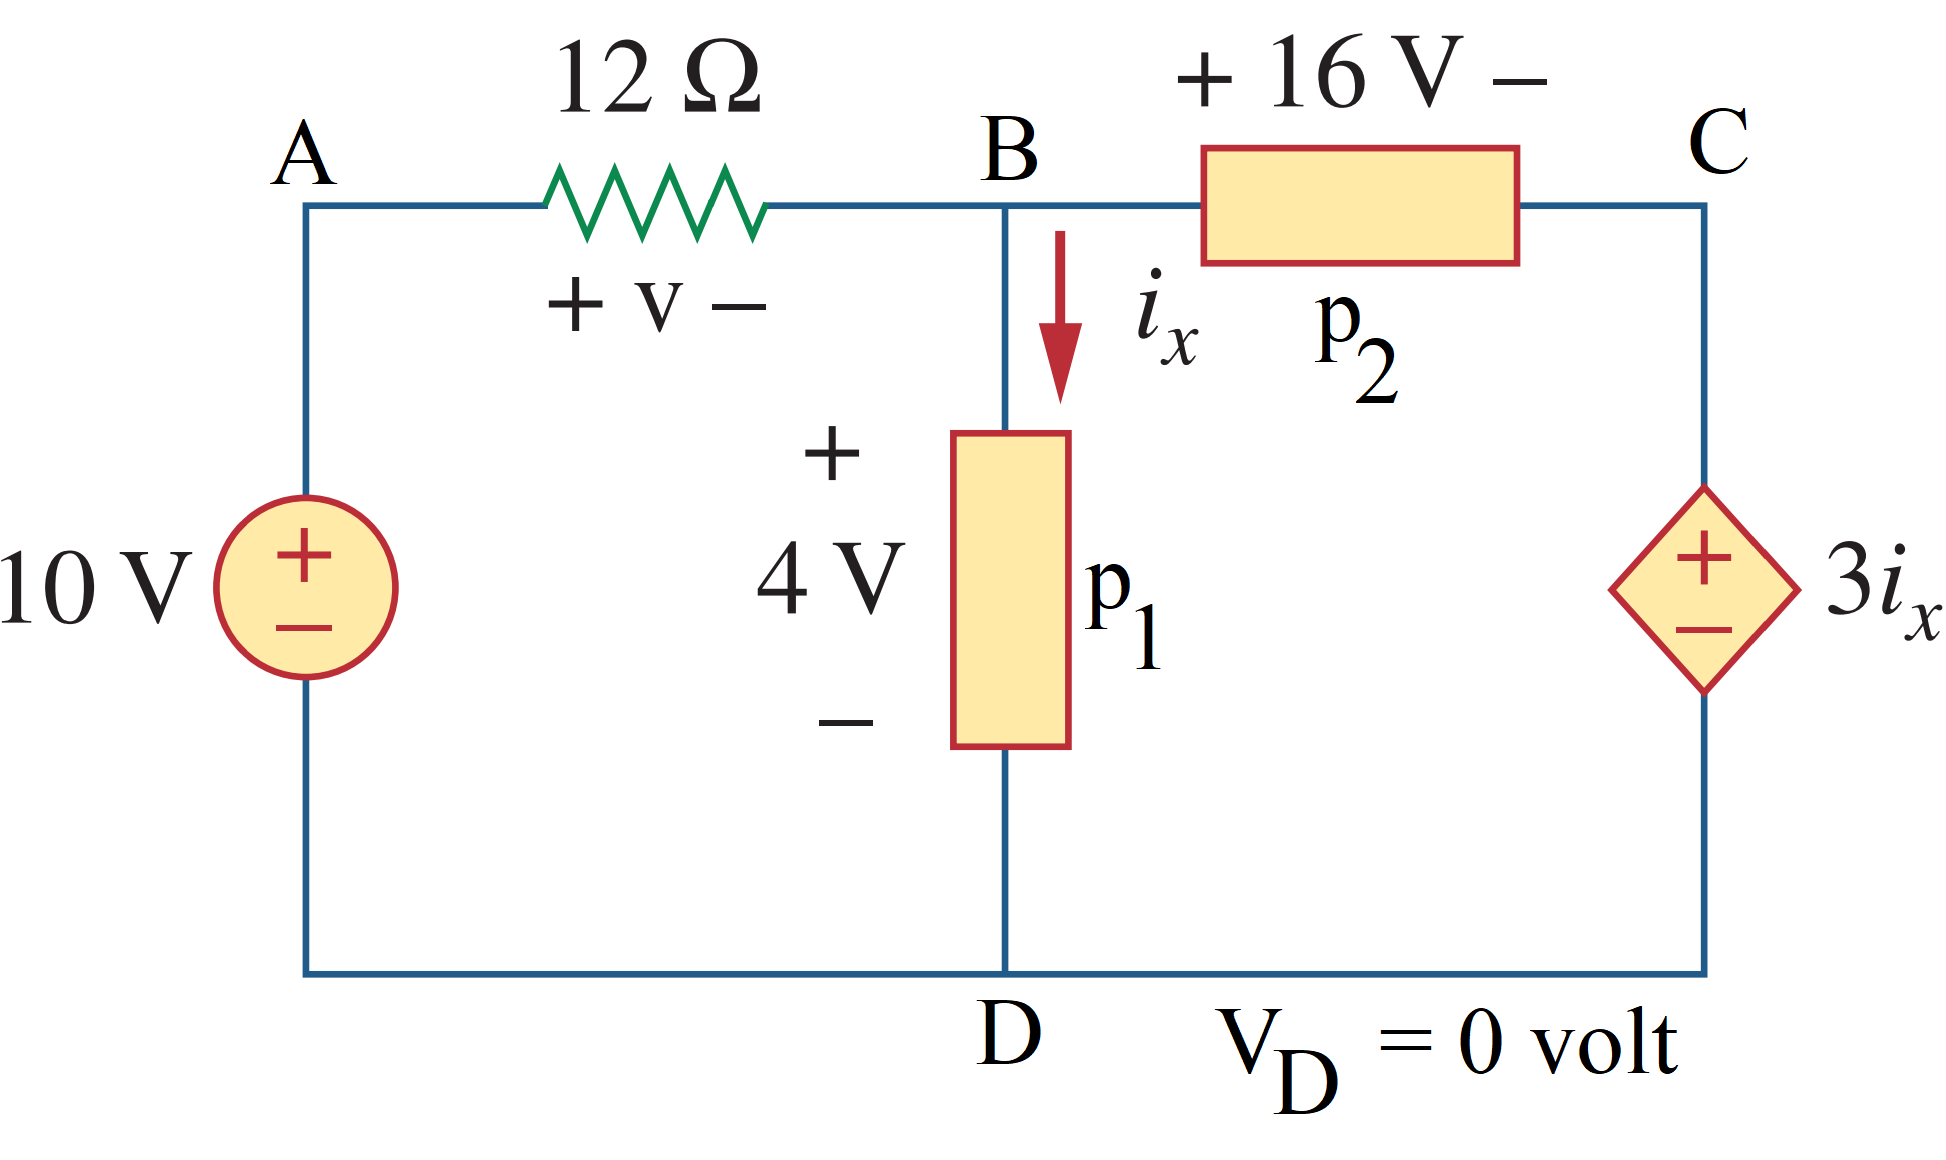
\includegraphics[width=8cm]{source/picture/bai_1/lab1_ex9_de.png}
    \caption{Find the unknown elements and variables, then check them out by simulation}
    \label{lab1_ex9_de}
\end{figure}

\subsubsection{Calculation}
\textit{\textbf{Notes:}}\\
\textit{Explanations, formulas, and equations are expected rather than only results.}\\

According to the: Kirchoff's Voltage Law \dotfill\bigskip\\
We have:\bigskip\\
$10 - v  - 4 = 0 \Rightarrow v = 6V$\dotfill\bigskip\\
$3i_x + 16 - 4  = 0 \Rightarrow i_x = -4 A$\dotfill\bigskip\\
So, we have:\bigskip\\
$p_1 = -4 \times 4 = -16$\dotfill $\longrightarrow$ active element.\bigskip\\
$I_{AB} = \frac{v}{12} = 0.5A$ \dotfill\bigskip\\
$I_{BC} = I_{AB} - i_x = 0.5 - (-4) = 4.5A$ \dotfill\bigskip\\
$p_2 = 4.5 \times 16 = 72(W)$\dotfill $\longrightarrow$  passive element.\bigskip\\
$U_{CD} = 3i_x = 3 \cdot (-4) = -12(V)$\dotfill\bigskip\

\subsubsection{Simulation}

\textbf{\textit{Tips:}}\\
To get the Current Controlled Voltage Source (CCVS) from the PSpice, under the \textit{\textbf{Place}} menu, find \textbf{\textit{PSpice Component > Source > Controlled Sources > CCVS}}.\\

A circuit used for the simulation in this exercise maybe like this:
\begin{figure}[H]
    \centering
    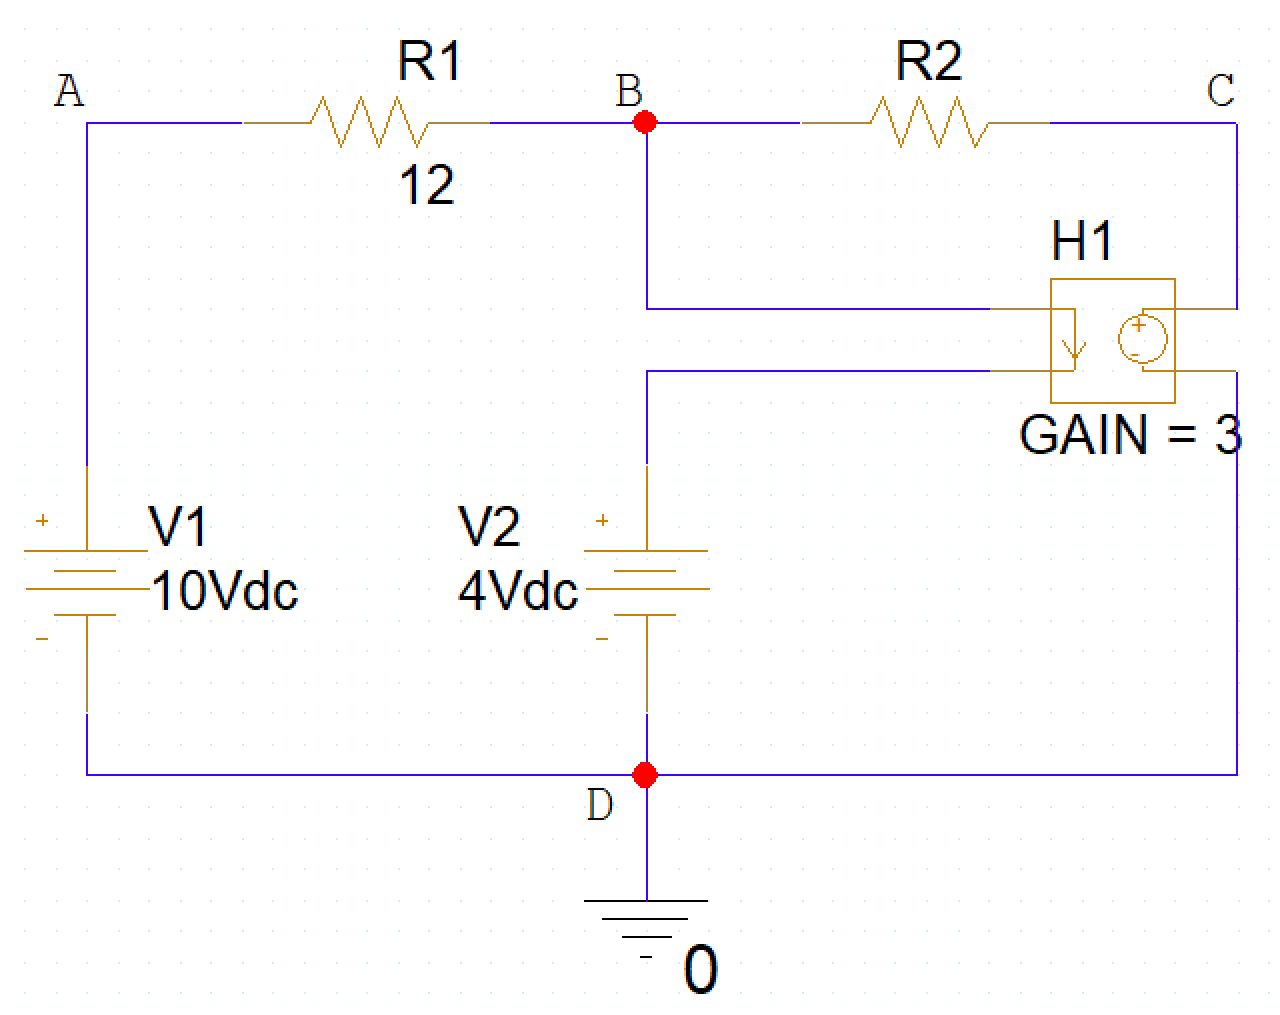
\includegraphics[width = 10cm]{source/picture/bai_1/lab1_ex9_ps.png}
    \caption{A circuit containing a Current Controlled Voltage Source in PSpice}
    \label{lab1_ex9_ps}
\end{figure}

\textit{\textbf{Simulation result (image):}}
\begin{figure}[H]
    \centering
    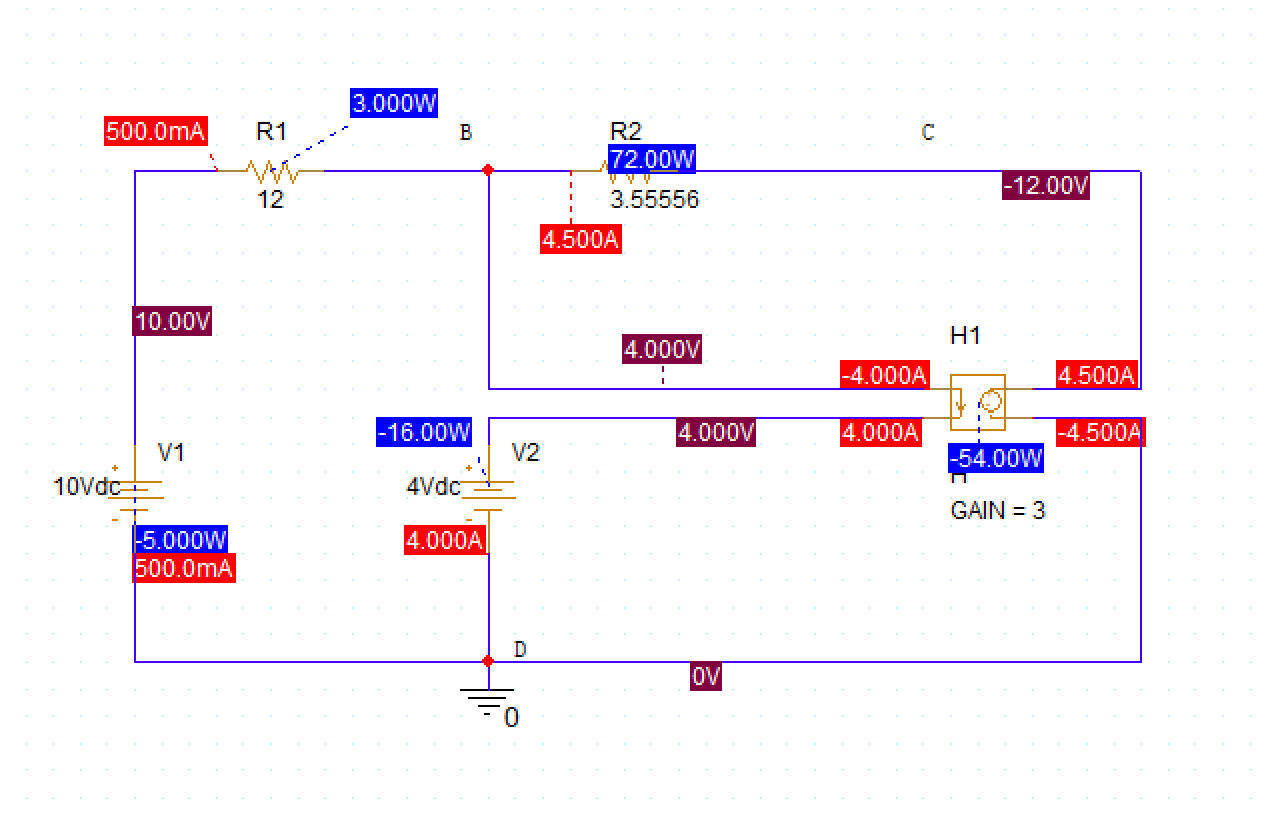
\includegraphics[width = 10cm]{source/picture/bai_1/ex9_sim.png}
\end{figure}
\newpage

\subsection{Exercise 10}
Given the following circuit. Find the voltage V. You can do this in any way but remember to explain it in detail. Then simulate the circuit to check the result.

\begin{figure}[H]
    \centering
    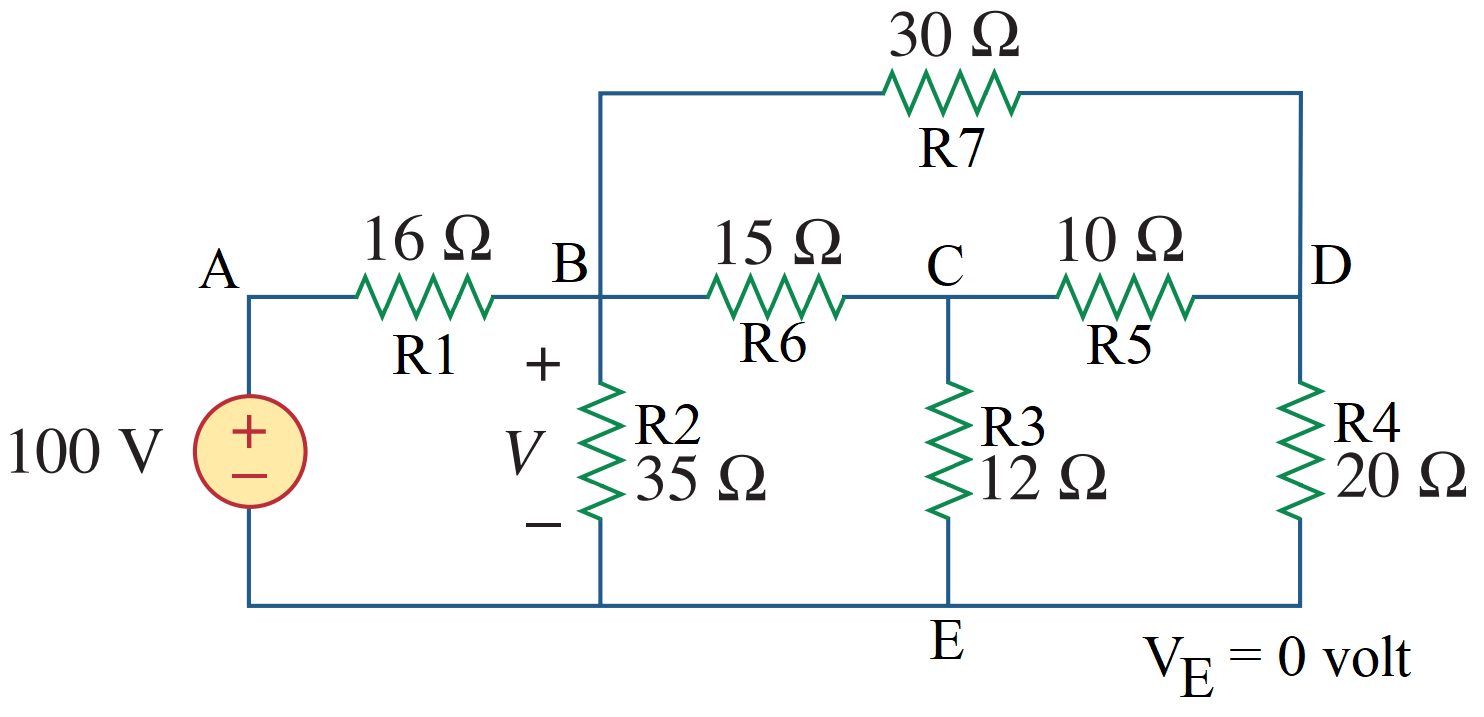
\includegraphics[width=9cm]{source/picture/bai_1/lab1_ex10_de.png}
    \caption{Find the voltage V}
    \label{lab1_ex10_de}
\end{figure}
Answer:
\begin{figure}[H]
    \centering
    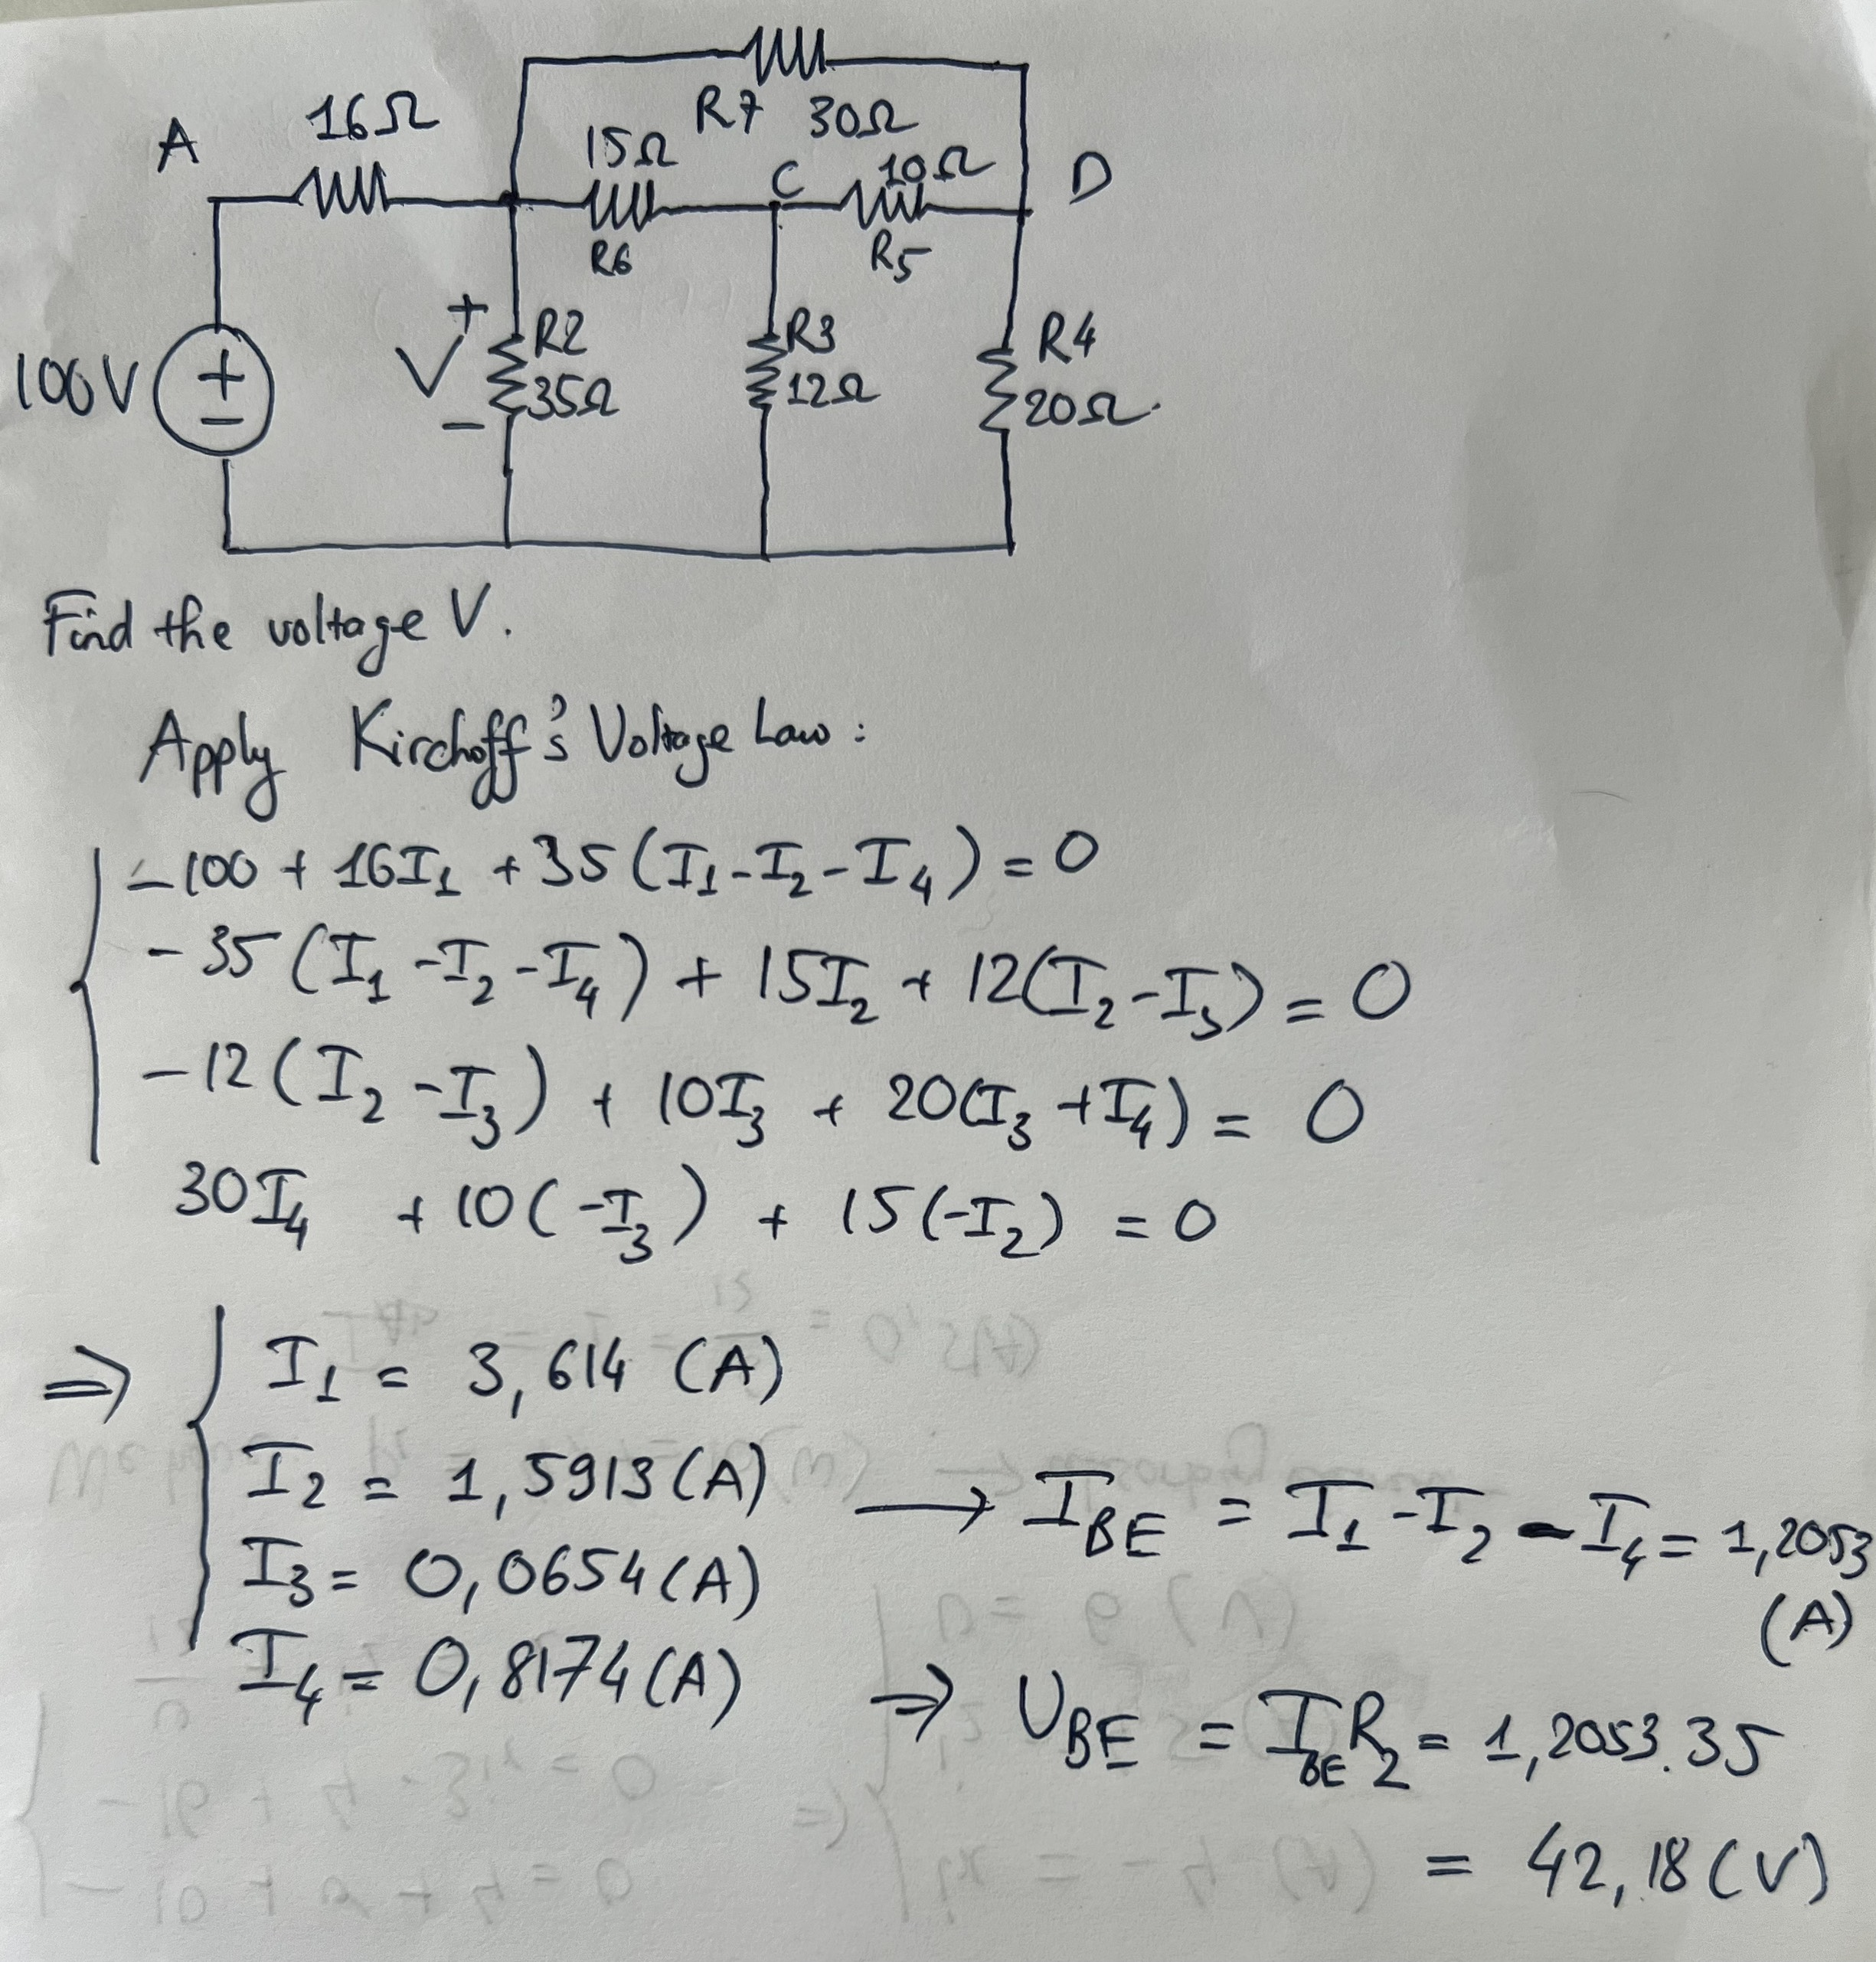
\includegraphics[width=9cm]{source/picture/bai_1/ex10_calculation.jpg}
\end{figure}

\bigskip\\
\textit{\textbf{Simulation result (image):}}
\begin{figure}[H]
    \centering
    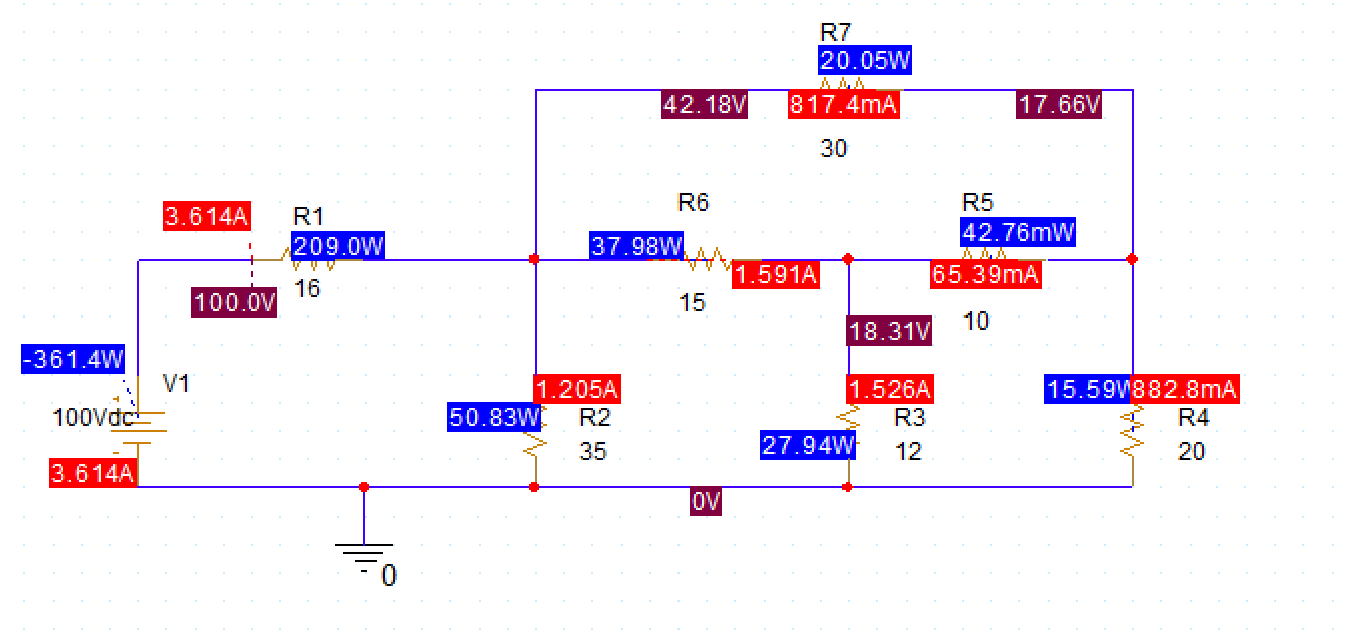
\includegraphics[width = 10cm]{source/picture/bai_1/ex10_sim.png}
\end{figure}



% \dotfill\medskip\par\mbox{}\dotfill

% \if\answer1
%   Provide the solution here
% \else
%   The solution is hide
% \fi \\
\chap{Diode Circuits Analysis}

\section{Introduction}
This laboratory exercise aims to demonstrate different diode wave shaping circuits. In general, these exercises aims to help students to fully understand how these diode circuit works in theory and actual situations. This laboratory exercises also helps students to understand about DC Sweep analysis and Time Domain (Transient) in simulation configuration.
\begin{itemize}
    \item DC Sweep analysis calculates the steady-state voltages and currents when sweeping a source, model parameter, global parameter, or temperature over a range of values. You can view the results of a DC sweep analysis in either a text output file or in the graphical display of the Probe window.
    \item Transient analysis involves a set of techniques used to analyze simulation data or experimental results in the time domain, specifically when the system under study is transitioning between two states
\end{itemize}
The targets are summarized as follows:
\begin{itemize}
    \item Create Project and design as provided schematic to analyse V-I characteristic with DC Sweep configuration.
    \item Analyse diode characteristic.
    \item Analyse some practical diode application circuits.
\end{itemize}
\newpage
\section{Diode simulation circuit}
In this manual, a simple circuit presented bellow is used in order to demonstrate  principles of a diode. Finally, the simulation based DC Sweep configuration is run to analyse the circuit.

\begin{figure}[!htp]
    \centering
    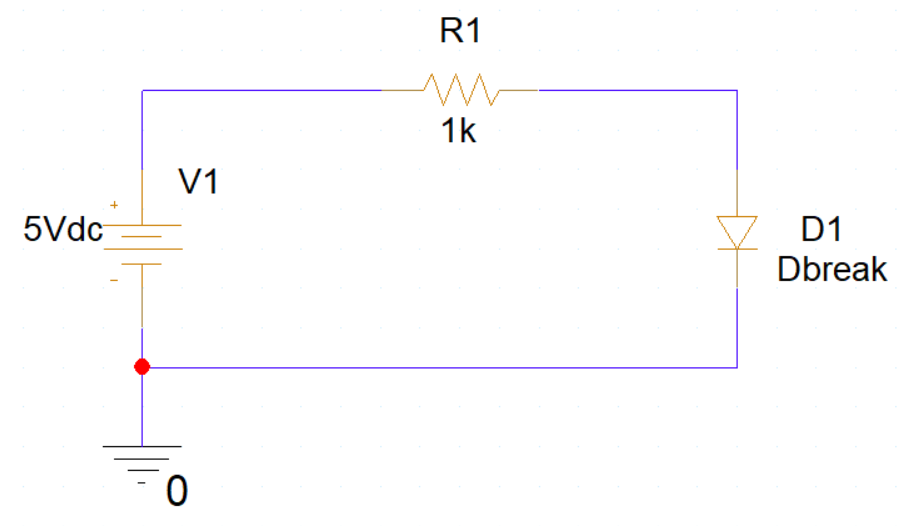
\includegraphics[width=4in]{source/picture/bai_2/diode_1.PNG}
    \caption{\textit{A simple simulation circuit using Diode}}
    \label{bai2_pic02}
\end{figure}


\textbf{Step 1: } Students are proposed to create a new project in PSPICE. Please select on the option \textbf{Create a blank project}.\\

\textbf{Step 2: } From the list of \textbf{Favorites} devices, search the component named \textbf{Dbreak}, which is a popular diode in circuit. Other components such as VDC, Resistor and the Ground, which are already used in Lab 1, are also added to the project as well. Finally, set the voltage supple of V1 to \textbf{5Vdc}.\\

\textbf{Step 3: } Create a simulation project by clicking on the menu \textbf{PSpice, New Simulation Profile}. After the name of the simulation profile is given, following dialog is shown:

\begin{figure}[!htp]
    \centering
    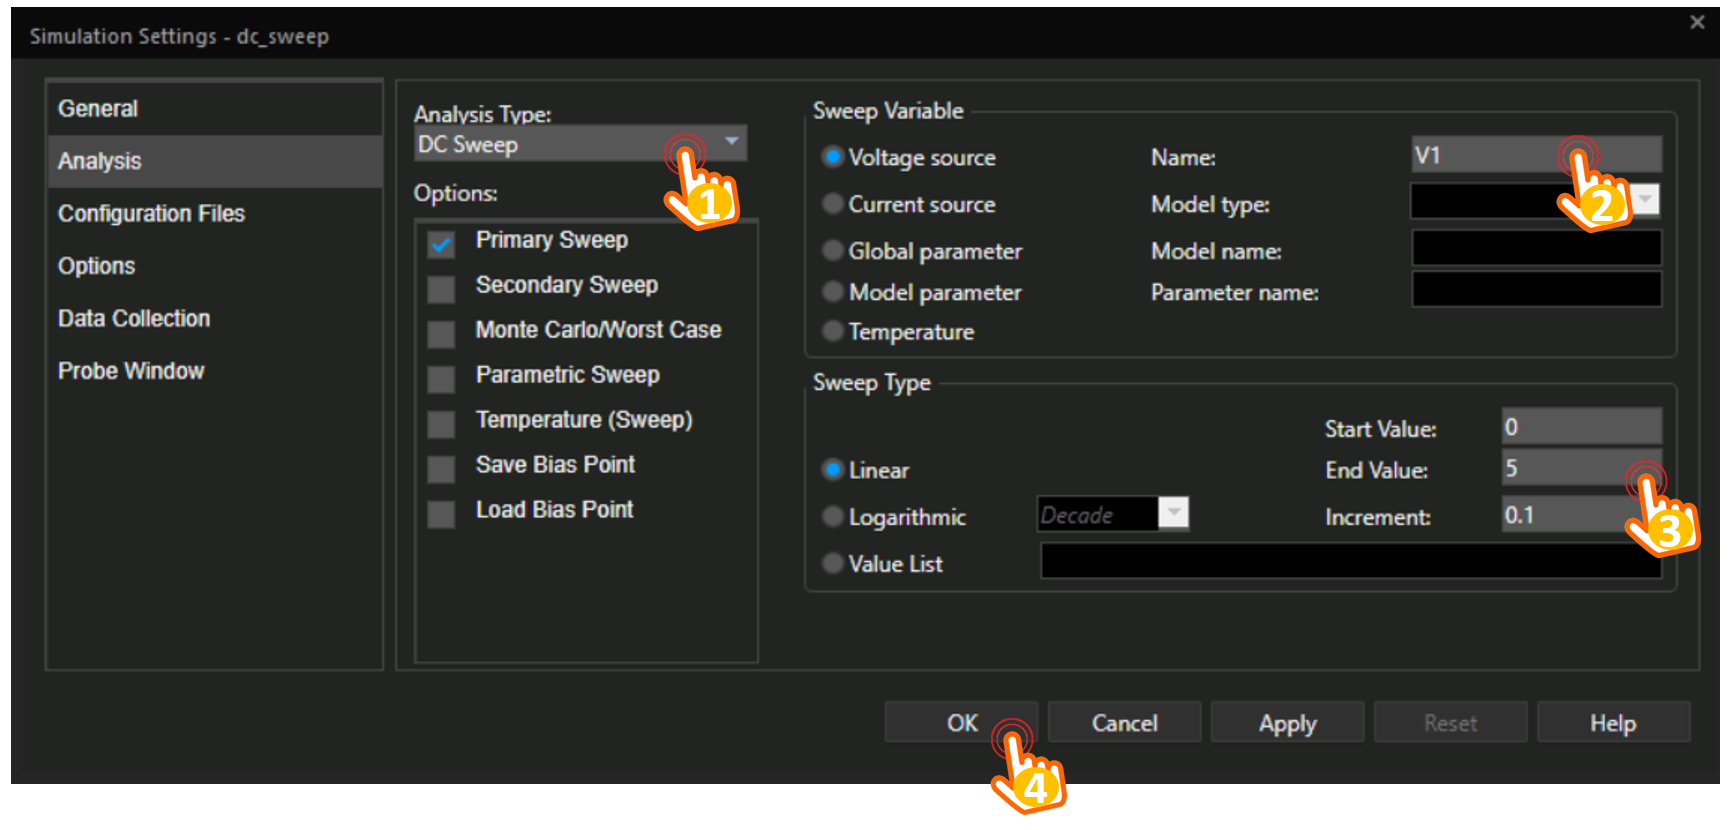
\includegraphics[width=4in]{source/picture/bai_2/diode_2.PNG}
    \caption{\textit{Configure the DC-Sweep simulation Profile}}
    \label{bai2_pic02_config}
\end{figure}


Following fields are required to configure:
\begin{itemize}
    \item \textbf{Analysis Type}: select \textbf{DC Sweep} mode
    \item \textbf{Sweep variable}: name of input source to analyze, which is (\textbf{V1}) in this case.
    \item \textbf{Sweep Type}: vary voltage of the source, which is from 0V to 5V and the incremental step is 0.1V.
\end{itemize}


\textbf{Step 5: } Run simulation (F11 or from menu \textbf{PSpice}, select \textbf{Run}). The simulation result for DC Sweep mode is launched as follows:

\begin{figure}[!htp]
    \centering
    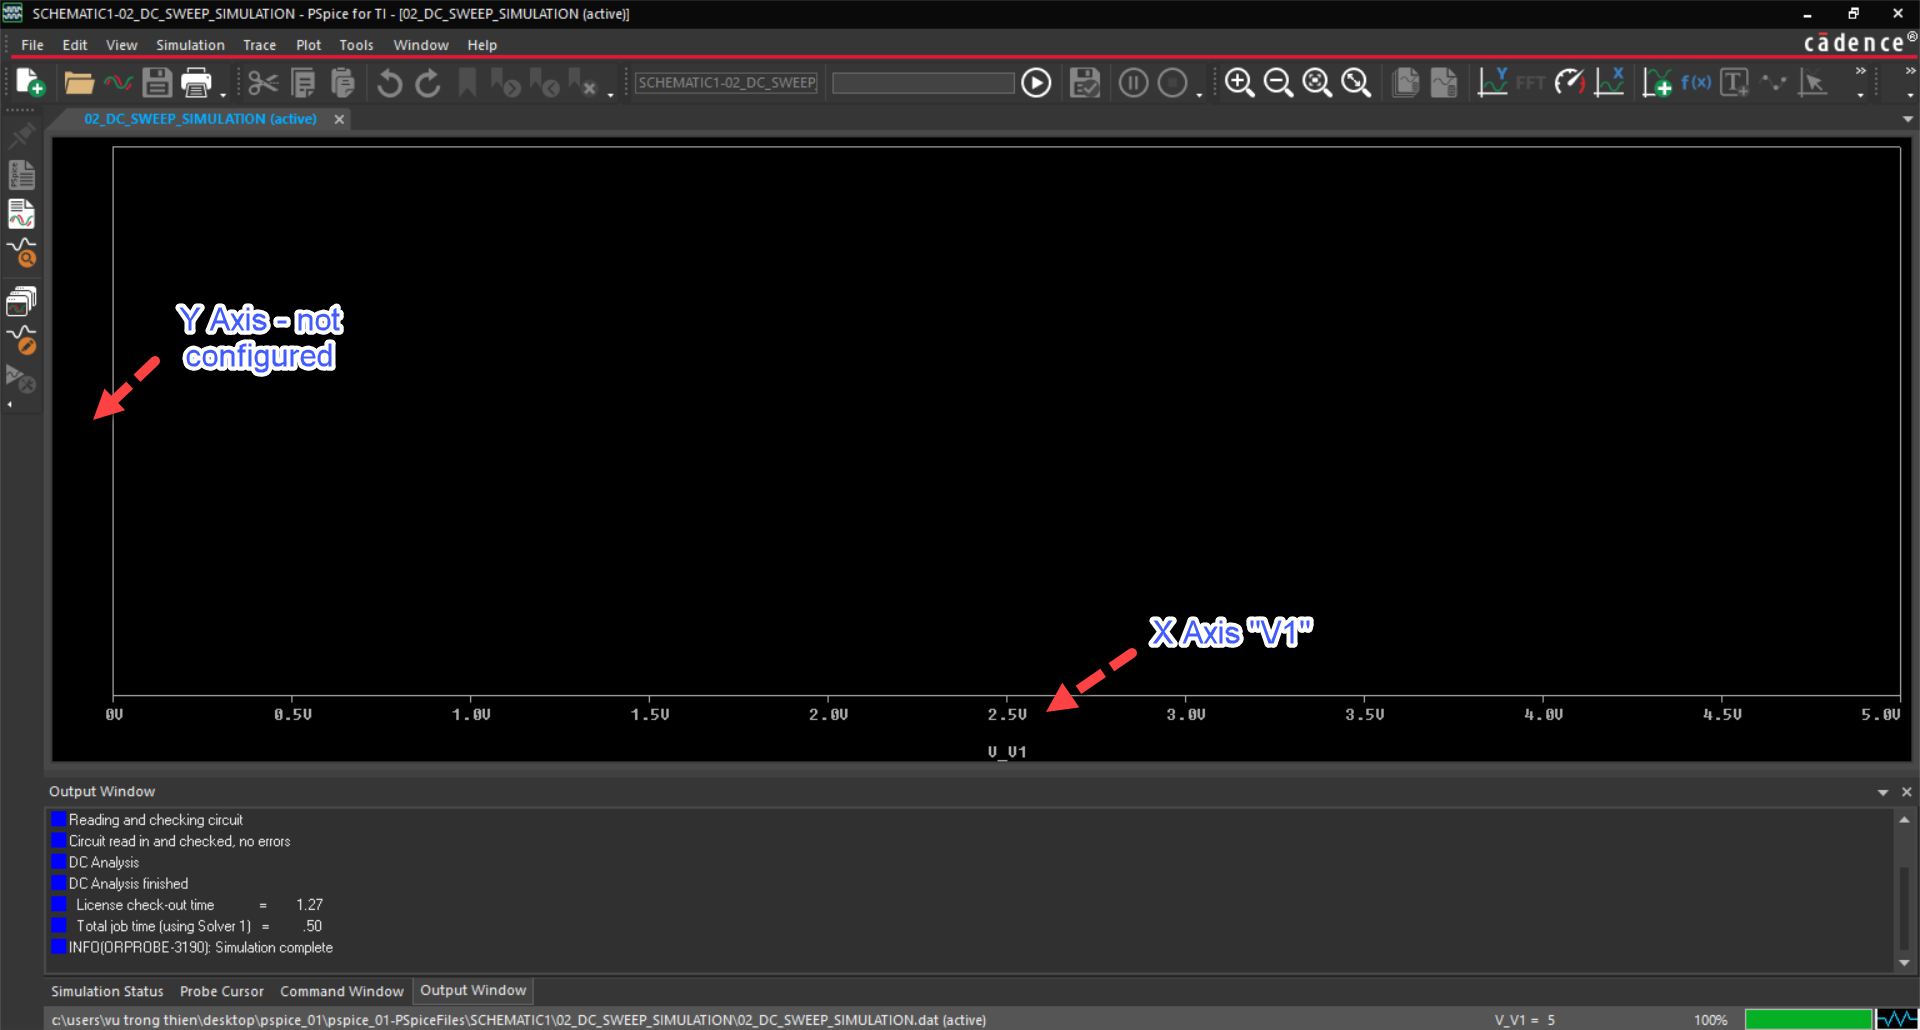
\includegraphics[width=4in]{source/picture/bai_2/12_RunSimulationNotConfigAxis.png}
    \caption{\textit{Simulation results for DC-Sweep mode}}
    \label{bai2_pic12}
\end{figure}

However, the screen is empty without any tracking information. In this case, we need to monitor the current in the circuit having a diode. To do this, from menu \textbf{Trace}, select \textbf{Add Trace} to open following dialog:

\begin{figure}[!htp]
    \centering
    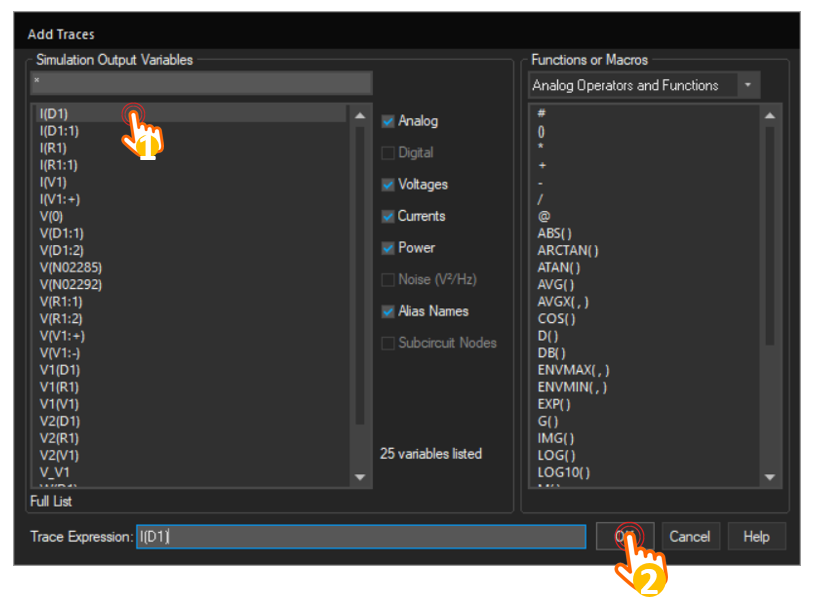
\includegraphics[width=4in]{source/picture/bai_2/14_ChooseID1ToYAxis.png}
    \caption{\textit{Add \textbf{I(D1)} to Y-Axis Trace}}
    \label{bai2_pic14}
\end{figure}

Choose \textbf{I(D1)} which is the current passing through the diode (and also the main current in the circuit having 2 components in a series). Finally, simulation results are depicted as follows:
\newpage
\begin{figure}[!htp]
    \centering
    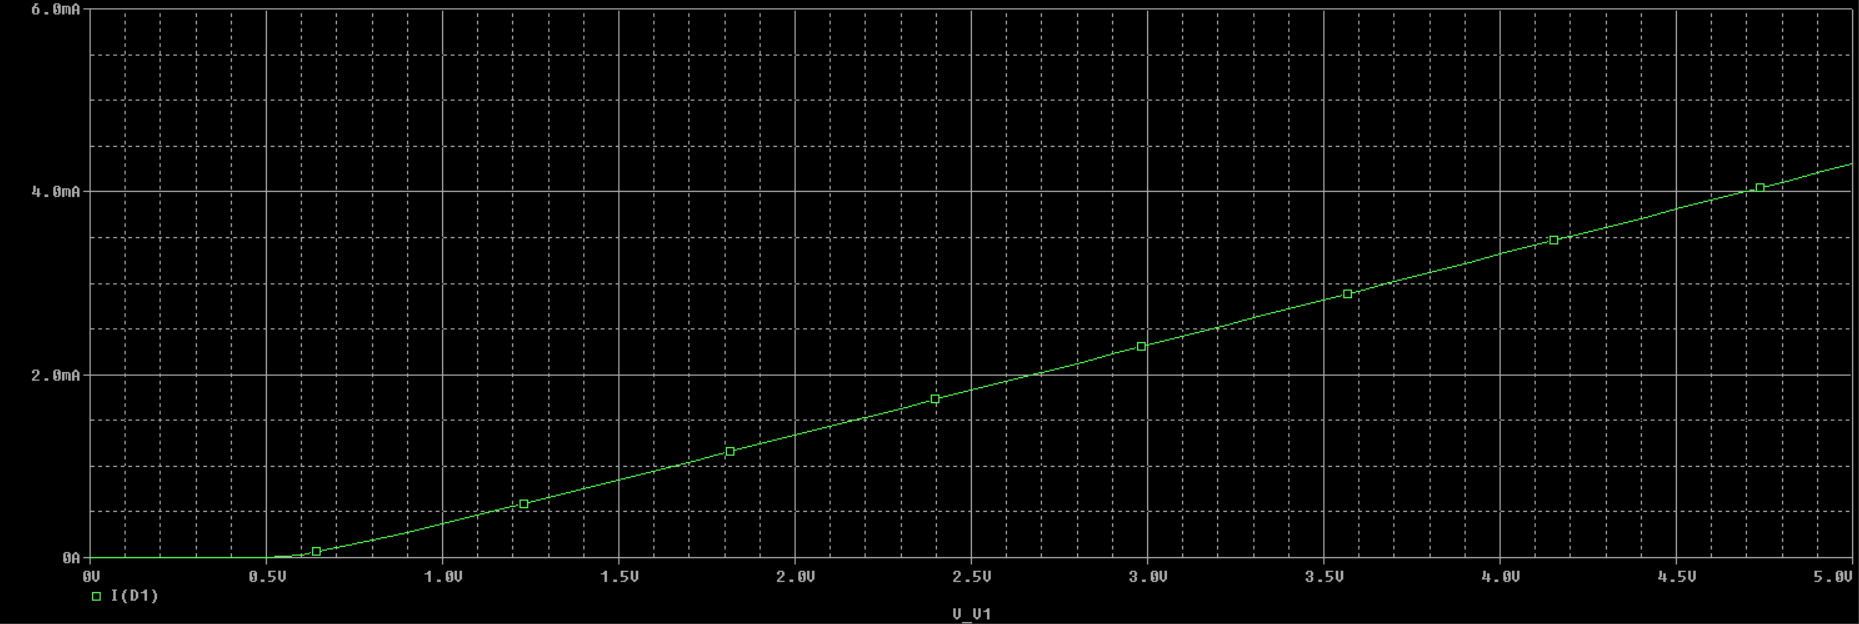
\includegraphics[width=5.5in]{source/picture/bai_2/15_ResultAfterAddYAxis.png}
    \caption{\textit{Simulation Result}}
    \label{bai2_pic15}
\end{figure}

\textbf{Step 6: } In order to make tracking information more readable, right click on the tracking line and choose \textbf{Trace Property} as follows:
\begin{figure}[!htp]
    \centering
    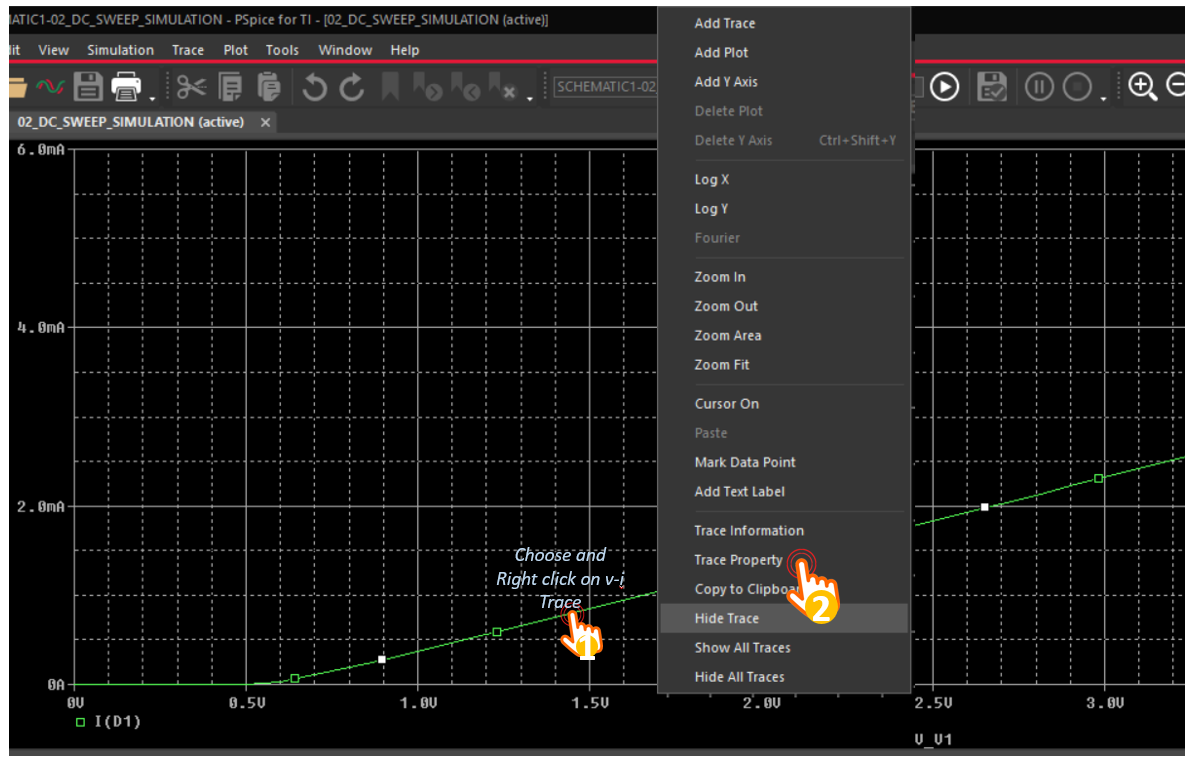
\includegraphics[width=4in]{source/picture/bai_2/16_ConfigTraceProperty.png}
    \caption{\textit{Configure Trace Property}}
    \label{bai2_pic16}
\end{figure}

The following dialog is opened, allow you to change the color and also the width of the tracking line

\begin{figure}[!htp]
    \centering
    \includegraphics[width=2in]{source/picture/bai_2/17_ChangeWidthTrace.png}
    \caption{\textit{Change Trace Width to make it more readable}}
    \label{bai2_pic17}
\end{figure}
\newpage
The final shape of the simulation result is look like the following picture:

\begin{figure}[!htp]
    \centering
    \includegraphics[width=5.5in]{source/picture/bai_2/18_ResultAfterConfigTrace.png}
    \caption{\textit{Simulation result after changing the Trace Width}}
    \label{bai2_pic18}
\end{figure}

The whole data for every point of the input voltage can be extract to text file by right click on the curve and select the option \textbf{Copy to Clipboard}. Finally, the data can be pasted to text editor, for instance, Notepad IDE.

\begin{figure}[!htp]
    \centering
    \includegraphics[width=3in]{source/picture/bai_2/diode_3.PNG}
    \caption{\textit{Extract data to Notepad Editor}}
    \label{bai2_pic18a}
\end{figure}

It is obviously that when the power supply is less than 0.7V, the current is close to zero (in order of $10^{-9}$ at 0.3V). However, when the input voltage is 1V, the current in the circuit is around 0.37mA. This result can be estimated as \textbf{(1V-0.7V)/1k}, when the practical diode model is applied. Students are proposed to check the simulation results at other points, such as V1 = 2V or V1 = 4V.\\


\textbf{Step 7: } A very important analysis with a diode is the relation between the voltage and the current across the diode, which is popular known as the V-I characteristic of the diode. To do this, on the simulation result windows, \textbf{double click on the X-Axis} to open the dialog as following:
\newpage
\begin{figure}[!htp]
    \centering
    \includegraphics[width=4in]{source/picture/bai_2/diode_14.PNG}
    \caption{\textit{Set the X-Axis of the simulation result}}
    \label{bai2_pic18b}
\end{figure}

Firstly, clicking on the \textbf{Add Variables} button and select \textbf{V(D1:1)}, which is the voltage across the diode. Secondly, on the data range, \textbf{select from 0V to 1V in the User Defined} option. Finally, add a trace from menu Trace, and select I(D1) as previous simulation. The figure bellow is achieved:

\begin{figure}[!htp]
    \centering
    \includegraphics[width=5.5in]{source/picture/bai_2/diode_15.PNG}
    \caption{\textit{V-I characteristic of a diode}}
    \label{bai2_pic18c}
\end{figure}

This figure confirms that in the forward bias mode, the drop-down voltage of a diode is around 0.7V, which is the default value in the practical diode model.

\textbf{Step 8: } The bias simulation is also applied in this lab. By clicking on menu \textbf{PSpice, New Simulation Profile}. Similar to the first lab, after providing the name for the simulation profile(e.g. bias\_point), only the analysis type is changed to \textbf{Bias Point}. Finally, click \textbf{OK} button to create the second simulation profile.
\newpage
\begin{figure}[!htp]
    \centering
    \includegraphics[width=4in]{source/picture/bai_2/diode_4.PNG}
    \caption{\textit{Add Bias Point simulation profile to the project}}
    \label{bai2_pic18d}
\end{figure}

Currently, there are two simulation profiles in the project, which can be browsed as following. In order to set a profile to active, right click on this profile and select \textbf{Make Active}.

\begin{figure}[!htp]
    \centering
    \includegraphics[width=3in]{source/picture/bai_2/diode_5.PNG}
    \caption{\textit{Set the active simulation profile}}
    \label{bai2_pic18e}
\end{figure}

Bias simulation results are displayed as follows:

\begin{figure}[!htp]
    \centering
    \includegraphics[width=4in]{source/picture/bai_2/21_EnableBiasCurrentDisplay.png}
    \caption{\textit{Enable Bias Current Display}}
    \label{bai2_pic21}
\end{figure}

From the simulation results, it is confirmed that the drop-down voltage of a diode is around 0.7V, which is very closed to the practical diode model.


\newpage
\section{Exercise and Report}
% Exercise 1: try above simulation circuit with other value of resistor to check voltage and current on circuit.
\subsection{Complete diode model}
According to the above simulation circuit (Figure 1.2), determine the voltage across the resistor and the diode ($V_{R}$, $V_{D}$), and also the current $I$ in the circuit with \textbf{two different values of R1}, including \textbf{220 Ohm} and \textbf{1.5K Ohm}. It is assumed that the complete diode model is used to analyse, having the forward voltage at \textbf{0.7V} and the internal resistor equal to \textbf{50 Ohm}.\\

Finally, the simulation on PSpice is run to double check with theory calculation. Brief explanations concerning the difference between theory and simulations can be provided in the report.\\

\subsubsection{Theory calculation}
\textit{\textbf{Notes:}}\\
\textit{Explanations, formulas, and equations are expected rather than only results.}\\

According to the: Ohm's Law and Complete diode model formula\bigskip\\
We have $V_{D}$: $I \cdot R_D + 0.7$\bigskip\\
Formula to calculate $V_{R}$: $ V_R = I \cdot R $\bigskip\\
Formula to calculate $I$: $I = \frac{V - 0.7}{R + r'_d}$\bigskip\\
Finally, when R = 220 Ohm, $V_{R} = I_{220} \cdot R = \frac{5-0.7}{220 + 50} \times 220 \approx 3.5037 (V)$ \bigskip\\
And when R = 1.5K Ohm, $V_{R} = I_{1.5K}\cdot R =\frac{5-0.7}{1500+50} \times 1500 \approx 4.16129 (V)) $ \bigskip\\


\subsubsection{PSpice Simulation}
Set the simulation profile to bias-point. Moreover, enable both \textbf{Enable Voltage Bias Display} and \textbf{Enable Current Bias Display} to show the simulation results. \\

Students are supposed to capture the screen in PSPice and present in this report.

\textit{\textbf{Simulation results (images)}}:\\ \textit{Your image goes here}
\begin{figure}[!htp]
    \centering
    \includegraphics[width = 500px]{source/picture/bai_2/sim_ex1.png}
\end{figure}
\newpage

\subsubsection{Comparison}
In this section, the theory calculations and PSpice simulations are summarized in the table bellow to compare the difference. Students are supposed to fill all information in the table.
\begin{center}
    \begin{tabular}{l|l|l|l|l|l|l|}
        \cline{2-7}
                                          & \multicolumn{3}{c|}{\textbf{Theory}} & \multicolumn{3}{c|}{\textbf{PSpice}}                          \\ \cline{2-7}
                                          & $V_R$                                & $V_D$                                & I      & $V_R$ & V & I \\ \hline
        \multicolumn{1}{|l|}{R = 220 Ohm} & 3.5037                               & 4.16129                              & 0.0159 &       &   &   \\ \hline
        \multicolumn{1}{|l|}{R= 1.5K Ohm} &                                      &                                      &        &       &   &   \\ \hline
    \end{tabular}
\end{center}


According to the above \textbf{Exercise Results}, give some comments about observation (between calculation results and simulation results):\dotfill\bigskip
\dotfill\bigskip\par\mbox{}\dotfill
\dotfill\bigskip\par\mbox{}\dotfill
\dotfill\bigskip\par\mbox{}\dotfill
\dotfill\bigskip\par\mbox{}\dotfill

% Exercise 2: Diode Series
\subsection{Diode in a series}
Similar to the previous exercise, determine the value of the voltage $V_{D1}$, $V_{D2}$, $V_{D3}$ and the current $I$ for the give circuit. Then, simulate again the circuit using PSpice. However, in this case, the practical diode model is used with the forward voltage is 0.7223V.\\

\begin{figure}[!htp]
    \centering
    \includegraphics[width = 4in]{source/picture/bai_2/Lab02_Ex_02.png}
    \caption{Find the voltage and the current in the given circuit}
    \label{lab02_ex02}
\end{figure}


\subsubsection{Theory Calculation}
\textit{\textbf{Notes:}}\\
\textit{Explanations, formulas, and equations are expected rather than only results.}\\

According to the:\dotfill\bigskip\\
We have $V_{D1}$ =\dotfill\bigskip\\
$V_{D2}$ =\dotfill\bigskip\\
$V_{D3}$ =\dotfill\bigskip\\
$V_{R1}$ = \dotfill\bigskip\\
Formula to calculate $I$: \dotfill\bigskip\\
$I$ = \dotfill\bigskip\\



\subsubsection{PSpice Simulation}
Set the simulation profile to bias-point. Moreover, enable both \textbf{Enable Voltage Bias Display} and \textbf{Enable Current Bias Display} to show the simulation results. \\

Students are supposed to capture the screen in PSPice and present in this report.

\textit{\textbf{Simulation results (images):}} \textit{Your image goes here}\\
\begin{figure}[!htp]
    \centering
    \includegraphics[width = 500px]{source/picture/bai_2/sim_ex2.png}
\end{figure}

\vspace{6cm}

\subsubsection{Comparison}

\begin{center}
    \begin{tabular}{l|l|l|l|l|l|}
        \cline{2-6}
                                          & \multicolumn{1}{c|}{$V_{D1}$} & \multicolumn{1}{c|}{$V_{D2}$} & \multicolumn{1}{c|}{$V_{D3}$} & \multicolumn{1}{c|}{$V_{R1}$} & \multicolumn{1}{c|}{$I$} \\ \hline
        \multicolumn{1}{|l|}{Calculation} &                               &                               &                               &                               &                          \\ \hline
        \multicolumn{1}{|l|}{PSpice}      &                               &                               &                               &                               &                          \\ \hline
    \end{tabular}
\end{center}

The circuit in this exercise is a simple solution to design a power supply by leveraging a voltage drop of a diode. For example, a SIM module used to send SMS messages has a good voltage supply at 4.3V. In this case, a diode is connected from a 5V supply (which is a very popular voltage) and then, connected to the module SIM. Not only used to protect the module to avoid reverse current, a diode is a low-cost solution to generate 4.3V power supply for the SIM module.

\subsection{Circuit Analysis with Diode}
In PSpice, some exercise in the lesson can be simulated to confirm the results. Although it is not exactly the same values (e.g. voltage and current), the simulation in PSpice is a tool to check your solution. An example simulation circuit having diode and resistors is depicted as follows:

\begin{figure}[!htp]
    \label{pic:halfwave_rectifier}
    \centering
    \includegraphics[width = 4in]{source/picture/bai_2/diode_10.PNG}
    \caption{Circuit analysis with diode}
    \label{lab02_ex031b}
\end{figure}

Students are proposed to analyse this circuit using practical diode model, with the drop-down voltage is around 0.7V. Then the simulation is run on PSpice to double check with your results.
\subsubsection{Theory calculation}
It is assumed that the voltage at anode and cathode of the diode $V_1$ and $V_2$. It is assumed that the diode is in forward bias mode.\\

According to the practical diode mode: $V_1$ -$V_2$ = 0.7V\\

Students are proposed to construct the equations to determine the current across all the resistors.

\dotfill\bigskip\par\mbox{}\dotfill
\dotfill\bigskip\par\mbox{}\dotfill
\dotfill\bigskip\par\mbox{}\dotfill
\dotfill\bigskip\par\mbox{}\dotfill
\subsubsection{PSpice simulation}
The bias point profile is used to run the simulation in this exercise. Students are proposed to capture the screen on PSpice showing the current and the voltage in the circuit.\\

\textit{Your image(s) goes here}\\
\begin{figure}[!htp]
    \centering
    \includegraphics[width = 500px]{source/picture/bai_2/sim_ex3.png}
\end{figure}
\newpage
\subsubsection{Comparison}
Students are supposed to summarized the results from both theory calculations and PSpice simulations and fill in the table bellow.\\

\begin{center}

    \begin{tabular}{l|l|l|l|l|l|l|l|l|l|l|l|l|}
        \cline{2-13}
                                      & \multicolumn{6}{c|}{\textbf{Theory Calculation}} & \multicolumn{6}{c|}{\textbf{PSpice Simulation}}                                                                                                                                                                    \\ \cline{2-13}
                                      & \multicolumn{1}{c|}{$I_{R1}$}                    & \multicolumn{1}{c|}{$I_{R2}$}                   & \multicolumn{1}{c|}{$I_{R3}$} & \multicolumn{1}{c|}{$I_{R4}$} & \multicolumn{1}{c|}{$V_{1}$} & $V_2$ & $I_{R1}$ & $I_{R2}$ & $I_{R3}$ & $V_{R4}$ & $V_1$ & $V_2$ \\ \hline
        \multicolumn{1}{|l|}{V = 8V}  &                                                  &                                                 &                               &                               &                              &       &          &          &          &          &       &       \\ \hline
        \multicolumn{1}{|l|}{V = 12V} &                                                  &                                                 &                               &                               &                              &       &          &          &          &          &       &       \\ \hline
    \end{tabular}

\end{center}

\subsection{Clamper Diode Circuit}
The circuits in the figure below are known as clampers or DC restorers. The simulation on PSpice is also shown in the figure below. These circuits clamp a peak of a waveform to a specific DC level (e.g. 0.7V). Students are supposed to implement the circuit in PSPice to verify their results from therory calculation.
\\
\begin{figure}[!htp]
    \label{pic:halfwave_rectifier1}
    \centering
    \includegraphics[width = 3.5in]{source/picture/bai_2/diode_11.PNG}
    \caption{Clamper circuit using diode}
    \label{lab02_ex031c}
\end{figure}

\subsubsection{Theory calculation}
In this part, it is assumed that the practical diode model is used. Present your equations to calculate three different currents, including $I_{R1}$, $I_{R2}$, $I_{D2}$ and the voltage $V_{R2}$.

\dotfill\bigskip\par\mbox{}\dotfill
\dotfill\bigskip\par\mbox{}\dotfill
\dotfill\bigskip\par\mbox{}\dotfill
\dotfill\bigskip\par\mbox{}\dotfill

\subsubsection{PSpice simulation}
The bias point simulation is run in PSpice. Capture your screen with voltage and current are enabled in the results.

\textit{Your image(s) goes here}\\
\begin{figure}[!htp]
    \centering
    \includegraphics[width = 500px]{source/picture/bai_2/sim_ex4.png}
\end{figure}

\vspace{8cm}

\subsubsection{Comparison}

Students are supposed to summarized the results from both theory calculations and PSpice simulations and fill in the table bellow.\\

\begin{center}

    \begin{tabular}{l|l|l|l|l|l|l|l|l|}
        \cline{2-9}
                                      & \multicolumn{4}{c|}{Theory calculation} & \multicolumn{4}{c|}{PSpice simulation}                                                                                                             \\ \cline{2-9}
                                      & \multicolumn{1}{c|}{$I_{R1}$}           & \multicolumn{1}{c|}{$I_{R2}$}          & \multicolumn{1}{c|}{$I_{D2}$} & \multicolumn{1}{c|}{$V_{R2}$} & $I_{R1}$ & $I_{R2}$ & $I_{D2}$ & $V_{R2}$ \\ \hline
        \multicolumn{1}{|l|}{V = 12V} &                                         &                                        &                               &                               &          &          &          &          \\ \hline
        \multicolumn{1}{|l|}{V = 20V} &                                         &                                        &                               &                               &          &          &          &          \\ \hline
    \end{tabular}
\end{center}

What can be concluded from this table?

\subsection{Power switching circuit}

The corruption of main power can be crucial in many different situations. For instance, when power is abruptly lost, you might want to save some backup data on a micro-controller. Such use cases need some form of automatic switching circuit to a secondary power source, such as a battery.\\

\newpage

\begin{figure}[!htp]
    \label{pic:halfwave_rectifier2}
    \centering
    \includegraphics[width = 3.5in]{source/picture/bai_2/diode_12.PNG}
    \caption{Power switching circuit}
    \label{lab02_ex031d}
\end{figure}

The simplest solution to this problem is simply to add a diode on each voltage source, as shown in the figure above. In this circuit, a 5V power supply can be used as a backup battery. Meanwhile, 9V is the main power supply for the system, which is demonstrated by a load resistor.\\

However, the main issue with this naive approach is that the voltage drop (forward voltage) across the diode might be too high for the system. Thanks to Schottky diode, this can be mitigated by using extremely low forward voltage one, which can be found on the market (e.g. Schottky diode having drop-down voltage around 250mV at 1A).

\subsubsection{Theory calculation}
In this part, it is assumed that the practical diode model is used. Present your equations to calculate the current $I_{D3}$, $I_{D4}$, $I_{RL}$ and the volatage $V_{RL}$ in three different cases: only 5V, only 9V and both 5V and 9V for the power supply.\\

\dotfill\bigskip\par\mbox{}\dotfill
\dotfill\bigskip\par\mbox{}\dotfill
\dotfill\bigskip\par\mbox{}\dotfill
\dotfill\bigskip\par\mbox{}\dotfill

\subsubsection{PSpice simulation}
The bias point simulation is run in PSpice with both power sources are enabled. Capture your screen with voltage and current are enabled in the results.\\

\textit{Your image(s) goes here}
\begin{figure}[!htp]
    \centering
    \includegraphics[width = 500px]{source/picture/bai_2/sim_ex5.png}
\end{figure}
\newpage
\vspace{8cm}

\subsubsection{Comparison}
Students are supposed to summarized the results from both theory calculations and PSpice simulations and fill in the table bellow. Both power sources are connected to the circuit.\\

\begin{center}
    \begin{tabular}{|l|l|l|l|l|l|l|l|}
        \hline
        \multicolumn{4}{|c|}{Theory calculation} & \multicolumn{4}{c|}{PSpice simulation}                                                                                                             \\ \hline
        \multicolumn{1}{|c|}{$I_{D1}$}           & \multicolumn{1}{c|}{$I_{D2}$}          & \multicolumn{1}{c|}{$I_{RL}$} & \multicolumn{1}{c|}{$V_{RL}$} & $I_{D1}$ & $I_{D2}$ & $I_{RL}$ & $V_{RL}$ \\ \hline
                                                 &                                        &                               &                               &          &          &          &          \\ \hline
                                                 &                                        &                               &                               &          &          &          &          \\ \hline
    \end{tabular}
\end{center}


The last feature of the diodes in this circuit is  to protect the reverse current in case both the power sources are switch on together. This use case is very popular when a micro-controller platform is programmed and powered by an USB port and also equipped with an adapter for external power supply.

% Exercise 3: Half-wave Rectifier.
% https://www.youtube.com/watch?v=A7pHAu2W5fE
\subsection{Half-wave Rectifier}\label{halfwaveRectifier}
In this exercise, an alternating source is used to generate a half-wave rectifier output using a diode. The schematic of the simulation is given bellow:

\begin{figure}[!htp]
    \label{pic:halfwave_rectifier3}
    \centering
    \includegraphics[width = 3.5in]{source/picture/bai_2/diode_6.PNG}
    \caption{Half-wave Rectifier with Voltage Sin Source}
    \label{lab02_ex031e}
\end{figure}

\textbf{Step 1: } Create the schematic.\\
The new component in this schematic is the \textbf{VSIN - Sine Voltage Source}, which can be found in the Favorites list. This component has four different parameters are required to configure, as follows:
\begin{itemize}
    \item VOFF: Offset voltage of the source
    \item VAMPL: Amplifier voltage of the source
    \item FREQ: Frequency of the alternative current
    \item AC: The source type (having value 0 or 1), to switch between VAC and VSIN. In VSIN source, the frequency can be modified.
\end{itemize}

After setting these parameters are set to the values shown in the figure above, add a voltage probe to track the output by clicking on the \textbf{Voltage/Level Marker} on the PSpice Toolbar, as follows:

\begin{figure}[!htp]
    \label{pic:halfwave_rectifier4}
    \centering
    \includegraphics[width = 5in]{source/picture/bai_2/diode_7.PNG}
    \caption{Add a voltage marker for simulation tracing}
    \label{lab02_ex031f}
\end{figure}

\textbf{Step 2: } Create a new simulation profile.
In order to generate the output signal of the voltage probe, the analysis type is set to \textbf{Time Domain (Transient)}. Moreover, due to the frequency of the power source is 50Hz, the \textbf{simulation time is set to 100ms}, to depict 10 cycles of the output signal. Finally, the resolution is set to 0.1ms in the \textbf{Maximum Step size}. The configuration windows for this simulation profile is presented as follows:

\begin{figure}[!htp]
    \label{pic:halfwave_rectifier5}
    \centering
    \includegraphics[width = 5in]{source/picture/bai_2/diode_8.PNG}
    \caption{Create Time Domain simulation profile}
    \label{lab02_ex031g}
\end{figure}


\textbf{Step 3: } Run the simulation and observe the results
Finally, run the simulation and the output on the simulation windows should be presented in  the figure bellow:

\begin{figure}[!htp]
    \label{pic:halfwave_rectifier6}
    \centering
    \includegraphics[width = 5in]{source/picture/bai_2/diode_9.PNG}
    \caption{Wave form for the half-ware rectifier circuit}
    \label{lab02_ex031h}
\end{figure}



\subsubsection{Theory calculation}
\textit{\textbf{Notes:}}\\
\textit{Explanations, formulas, and equations are expected rather than only results.}\\

\textbf{\textit{Approximation:}} Diodes have $V_f$ = 0.78V\\
\begin{itemize}
    \item Minimum Value of $V_{R1}$ = \dotfill\\
    \item Maximum Value of $V_{R1}$ = \dotfill\\
    \item Duration (millisecond) for a cycle of $V_{R1}$ = \dotfill\\
\end{itemize}

\subsubsection{PSpice simulation}
Export your simulation results to Notepad for instance, and find the minimum and the maximum point of the output voltage, then fill your answer to the section bellow:

\begin{itemize}
    \item Minimum Value of $V_{R1}$ = \dotfill\\
    \item Maximum Value of $V_{R1}$ = \dotfill\\
    \item Duration (millisecond) for a cycle of $V_{R1}$ = \dotfill\\
\end{itemize}

The tracking point can also be used directly on the simulation output windows, by the \textbf{Toggle Cursor} option on the toolbar. A Probe Cursor window is opened to update a tracking point.

% Exercise 4: Full-wave Rectifier.

% Given the following circuit. Simulate circuit to understand more about Half-wave Rectifier Application of Diode.

% \begin{figure}[!htp]
%     \centering
%     \includegraphics[width = 7cm]{source/picture/bai_2/Lab02_Ex032_HalfwaveRectifierWithTransformer.png}
%     \caption{Half-wave Rectifier with Input V Sin Source and Transformer}
%     \label{lab02_ex032}
% \end{figure}
% \textbf{Tips:}\\
% \begin{itemize}
%     \item To place \textbf{ Transformer}, choose \textbf{Place > Pspice Components... > Model Application... > System Modules > Transformer}
%     \item Configure \textbf{Transformer} as \textbf{Two Winding}
% \end{itemize}

\subsection{Full-wave Rectifier}
The following circuit is known as a full-wave bridge diode rectifier. Given that the transformer has the ratio $N1/N2 = 10$. Write the voltage difference equation $V_{AB}$ and $V_{CD}$. After that, perform a time-domain (transient) analysis to check the equation you've written.

\begin{figure}[H]
    \centering
    \includegraphics[width=5in]{source/picture/bai_2/LAB2_EX4_de.png}
    \caption{Full-wave bridge rectifier}
    \label{lab2_ex4_de}
\end{figure}

\textbf{\textit{Tips 1:}}
To place the component \textbf{transformer}:
\begin{itemize}
    \item \textbf{Step 1:} Go to \textbf{\textit{Place > PSpice Component > Modeling Application...}}
    \item \textbf{Step 2}: Browse for the \textbf{\textit{Transformer}} component under the \textbf{\textit{System Modules}} category as shown in the following Figure.
          \begin{figure}[H]
              \centering
              \includegraphics[width=5cm]{source/picture/bai_2/PSpicePlaceTransformer.png}
              \caption{Browse for the component \textbf{Transformer}}
              \label{pspicePlaceTransformer}
          \end{figure}
    \item \textbf{Step 3:} Set the transformation ratio before placing as shown below.
          \begin{figure}[H]
              \centering
              \includegraphics[width=15cm]{source/picture/bai_2/PSpiceTransformerSetting.png}
              \caption{Setting the transformation ratio before placing the transformer}
              \label{pspiceTransformerSetting}
          \end{figure}
\end{itemize}

\textbf{\textit{Tips 2:}}
The Voltage Differential Markers in PSPICE for TI:
\begin{figure}[H]
    \centering
    \includegraphics[width=12cm]{source/picture/bai_2/voltageDifferenceMarkers.png}
    \caption{The Voltage Differential Markers in PSPICE for TI}
    \label{vDiffMkrPair}
\end{figure}

\subsubsection{Theory calculation}
\textit{\textbf{Notes:}}\\

\textit{Explanations, formulas, and equations are expected rather than only results.}\\
\\
\textbf{\textit{Approximation:}} \textit{Diodes have $V_f$ = 0.7V}\bigskip\\
\\
$V_{AB} = $ \dotfill\bigskip\\
\\
$V_{CD} = $ \dotfill\bigskip\\


\subsubsection{Simulation}
The sinusoidal waveform of the voltage difference $V_{AB}$ has the period $T = $ \dotfill\\
If we want to perform the transient analysis in 10 periods of the waveform $V_{AB}$, the required time would be:\dotfill\\
If we want the sampling rate to be as ten times higher than the frequency of the sinusoidal voltage difference $V_{AB}$, the time interval between two consecutive sampling time points should be:\dotfill\bigskip\\
\\
Now, create a simulation profile as guided in the \textbf{Exercise \ref{halfwaveRectifier}} and perform your simulation to check it out!\\

\textbf{\textit{Simulation result:}}
Show both $V_{AB}$ and $V_{CD}$ in a single plot window to illustrate the relationship between them. Don't forget to use the cursors to prove that the equation you've written is correct.\\
\\
\textit{(Your image(s) goes here)}\\
\begin{figure}[H]
    \centering
    \includegraphics[width=500px]{source/picture/bai_2/ex7_sim.png}
\end{figure}

\\
\\
\begin{figure}[H]
    \centering
    \includegraphics[width=500px]{source/picture/bai_2/ex7_plot.png}
\end{figure}
\newpage

\subsection{Zener Diode as a Regulator}
The Zener diode has a well-defined reverse-breakdown voltage, at which it starts conducting current, and continues operating continuously in the reverse-bias mode without getting damaged. Additionally, the voltage drop across the diode remains constant over a wide range of voltages, a feature that makes Zener diodes suitable for use in voltage regulation.

\begin{figure}[!htp]
    \centering
    \includegraphics[width = 4in]{source/picture/bai_2/zener_3.PNG}
    \caption{Electrical characteristic of Zener diode}
    \label{lab02_zener1}
\end{figure}

In this exercise, a Zener diode is used to design a voltage regular circuit. The schematic in this exercise is given following:

\begin{figure}[!htp]
    \centering
    \includegraphics[width = 4in]{source/picture/bai_2/zener_1.PNG}
    \caption{Voltage regulator using Zener diode}
    \label{lab02_zener2}
\end{figure}

The Zener component in the circuit can be found in the Favourites list by search the keyword \textbf{Zener}. The full name of the component used in the circuit above is \textbf{Zenner\_P - Zener Diode (parameterized)}. The default Zener voltage of this component is $V_Z = 5V$. However, this value can be changed in the properties of the component (right click and select Edit Properties) for other simulations. \\

For theory calculation, students are supposed to provide equations for these values
\begin{itemize}
    \item $I_{L}$ = \dotfill\\
    \item $I_{S}$ = \dotfill\\
    \item $I_{Z}$ = \dotfill\\
    \item $P_{RS}$ = \dotfill\\
    \item $P_{Z}$ = \dotfill\\
\end{itemize}

Then, perform the calculation for the Zener diode voltage regulator with two different input voltage, including 8V and 12V power supply. Finally, run the simulations in PSpice (in \textbf{Bias Point} simulation profile) to confirm with the theory calculation. \\

The results are summarized in the table bellow.

\begin{center}
    \begin{tabular}{l|l|l|l|l|l|l|l|l|l|l|l|l|}
        \cline{2-13}
                                        & \multicolumn{6}{c|}{\textbf{Theory Calculation}} & \multicolumn{6}{c|}{\textbf{PSpice Simulation}}                                                                                                                                                      \\ \cline{2-13}
                                        & \multicolumn{1}{c|}{$I_S$}                       & \multicolumn{1}{c|}{$I_L$}                      & \multicolumn{1}{c|}{$I_Z$} & \multicolumn{1}{c|}{$V_L$} & \multicolumn{1}{c|}{$P_{RS}$} & $P_Z$ & $I_S$ & $I_L$ & $I_Z$ & $V_L$ & $P_{RS}$ & $P_Z$ \\ \hline
        \multicolumn{1}{|l|}{Vcc = 8V}  &                                                  &                                                 &                            &                            &                               &       &       &       &       &       &          &       \\ \hline
        \multicolumn{1}{|l|}{Vcc = 12V} &                                                  &                                                 &                            &                            &                               &       &       &       &       &       &          &       \\ \hline
    \end{tabular}
\end{center}

% % Exercise 5: Clipper Application.
% \subsection{Exercise 5: Clipper}
% Given the following circuit. Simulate circuit to understand more about Clipper Application of Diode.
% \begin{figure}[!htp]
%     \centering
%     \includegraphics[width = 7cm]{source/picture/bai_2/Lab02_Ex05_Clipper_01.png}
%     \caption{Negative Peak Clipper}
%     \label{lab02_ex051}
% \end{figure}
% \begin{figure}[!htp]
%     \centering
%     \includegraphics[width = 7cm]{source/picture/bai_2/Lab02_Ex05_Clipper_02.png}
%     \caption{Symmetrical Clipper}
%     \label{lab02_ex052}
% \end{figure}
% \begin{figure}[!htp]
%     \centering
%     \includegraphics[width = 7cm]{source/picture/bai_2/Lab02_Ex05_Clipper_03.png}
%     \caption{Clipper with DC Source}
%     \label{lab02_ex053}
% \end{figure}

% \newpage
% \subsubsection{Calculation}
% \textit{\textbf{Notes:}}\\
% \textit{Explanations, formulas, and equations are expected rather than only results.}\\
% \\
% \textbf{\textit{Approximation:}} \textit{Diodes have $V_f$ = 0.7V and $r_d$ = 0 Ohm}\\
% \begin{itemize}
%     \item Minimum Value of $V_{out1}$ = \dotfill\\
%     \item Maximum Value of $V_{out1}$ = \dotfill\\
%     \item \textbf{Explanation} for value of \textbf{$V_{out1}$}: \dotfill\bigskip\\
%     \item Minimum Value of $V_{out2}$ = \dotfill\\
%     \item Maximum Value of $V_{out2}$ = \dotfill\\
%      \item \textbf{Explanation} for value of \textbf{$V_{out2}$}: \dotfill\bigskip\\
%     \item Minimum Value of $V_{out3}$ = \dotfill\\
%     \item Maximum Value of $V_{out4}$ = \dotfill\\  
%      \item \textbf{Explanation} for value of \textbf{$V_{out3}$}: \dotfill\bigskip\\
% \end{itemize}

% \textit{\textbf{Simulation results (check simulation values and images):}}
% \begin{itemize}
%     \item Minimum Value of $V_{out1}$ = \dotfill\\
%     \item Maximum Value of $V_{out1}$ = \dotfill\\
%     \item \textbf{Explanation} for value of \textbf{$V_{out1}$}: \dotfill\bigskip\\
%     \item Minimum Value of $V_{out2}$ = \dotfill\\
%     \item Maximum Value of $V_{out2}$ = \dotfill\\
%      \item \textbf{Explanation} for value of \textbf{$V_{out2}$}: \dotfill\bigskip\\
%     \item Minimum Value of $V_{out3}$ = \dotfill\\
%     \item Maximum Value of $V_{out4}$ = \dotfill\\  
%      \item \textbf{Explanation} for value of \textbf{$V_{out3}$}: \dotfill\bigskip\\
% \end{itemize}

% \textbf{Simulation Images}\\
% Diagrams \textbf{Time Domain (Transient)} to display relationship between input voltage and output voltage for each circuit.

% % Exercise 6: Clampers Application.
% \subsection{Exercise 6: Clamper Application}
% Given the following circuit. Simulate circuit to understand more about Clampers Application of Diode.
% \begin{figure}[!htp]
%     \centering
%     \includegraphics[width = 7cm]{source/picture/bai_2/Lab02_Ex061.png}
%     \caption{Positive Clamper}
%     \label{lab02_ex061}
% \end{figure}
% \begin{figure}[!htp]
%     \centering
%     \includegraphics[width = 7cm]{source/picture/bai_2/Lab02_Ex062.png}
%     \caption{Positive Clamper with Source DC 3Vdc}
%     \label{lab02_ex062}
% \end{figure}
% \begin{figure}[!htp]
%     \centering
%     \includegraphics[width = 7cm]{source/picture/bai_2/Lab02_Ex063.png}
%     \caption{Negative Clamper}
%     \label{lab02_ex063}
% \end{figure}
% \begin{figure}[!htp]
%     \centering
%     \includegraphics[width = 7cm]{source/picture/bai_2/Lab02_Ex064.png}
%     \caption{Nagative Clamper with Source DC 3Vdc}
%     \label{lab02_ex064}
% \end{figure}

% \subsubsection{Calculation and Explanation}
% \textit{\textbf{Notes:}}\\
% \textit{Explanations, formulas, and equations are expected rather than only results.}\\
% \textbf{Approximation: }: Diodes have $V_f$ = 0.7V and $r_d$ = 0 Ohm\\

% \textbf{Simulation Images}\\
% Diagrams \textbf{Time Domain (Transient)} to display relationship between input voltage and output voltage for each circuit.
% \begin{itemize}
%     \item Capture simulation diagram for each circuit
%     \item \textbf{Analyze} briefly circuit (for each diagram) 
% \end{itemize}

% Exercise 7: AC/DC Power Circuit Application.
\subsection{AC/DC Power Circuit Application}
In this exercise, we are building step by step an AC to DC voltage source transformation circuit. Students perform a time-domain simulation and write out comments and explanations for each step.\\
\\
\textbf{\textit{Tips: }} To place a capacitor, go to \textbf{\textit{Place > PSpice Component > Capacitor}}

\begin{itemize}
    \item \textbf{Step 1:} The rectified voltage without any filtering or being regulated.  \begin{figure}[H] \centering \includegraphics[width=\linewidth]{source/content/lab2_ex9_step1.png} \caption{The rectified voltage without any filtering or being regulated} \label{lab2_ex9_step1} \end{figure} \textit{\textbf{Simulation result:}} \textit{Your image goes here}\\ \\ \vspace{8cm} \\ \textbf{\textit{Any comments or explanations:}} \dotfill\bigskip\par\mbox{}\dotfill \dotfill\bigskip\par\mbox{}\dotfill \dotfill\bigskip\par\mbox{}\dotfill \dotfill\bigskip\par\mbox{}\dotfill \dotfill\bigskip\par\mbox{}\dotfill \dotfill\bigskip\par\mbox{}\dotfill \item \textbf{Step 2:} Rectified voltage regulated with a $10\micro F$ capacitor.  \begin{figure}[H] \centering \includegraphics[width=\linewidth]{source/content/lab2_ex9_step2.png} \caption{Rectified voltage regulated with a capacitor} \label{lab2_ex9_step2} \end{figure} \textit{\textbf{Simulation result(s):}} \textit{Your image goes here}\\ \\ \vspace{8cm} \\ \textbf{\textit{Any comments or explanations:}} \dotfill\bigskip\par\mbox{}\dotfill \dotfill\bigskip\par\mbox{}\dotfill \dotfill\bigskip\par\mbox{}\dotfill \dotfill\bigskip\par\mbox{}\dotfill \dotfill\bigskip\par\mbox{}\dotfill \dotfill\bigskip\par\mbox{}\dotfill \item \textbf{Step 3}: Replace the $10\micro F$ capacitor with a $680\micro F$ one and re-run the simulation, recognize the change in the result and explain.\\ \textit{\textbf{Simulation result(s):}} \textit{Your image goes here}\\ \\ \vspace{6cm} \\ \textbf{\textit{Any comments or explanations:}} \dotfill\bigskip\par\mbox{}\dotfill \dotfill\bigskip\par\mbox{}\dotfill \dotfill\bigskip\par\mbox{}\dotfill \dotfill\bigskip\par\mbox{}\dotfill \dotfill\bigskip\par\mbox{}\dotfill \dotfill\bigskip\par\mbox{}\dotfill \item \textbf{Step 4:} Add a zener diode as in Figure \ref{lab2_ex9_step3} with the $zener voltage$ properties set to 22 volt then simulate the circuit and comment or explain the result.  \begin{figure}[H] \centering \includegraphics[width=\linewidth]{source/content/lab2_ex9_step3.png} \caption{Rectified voltage regulated with a capacitor and a zener diode} \label{lab2_ex9_step3} \end{figure} \textit{\textbf{Simulation result(s):}} \textit{Your image goes here}\\ \\ \vspace{8cm} \\ \textbf{\textit{Any comments or explanations:}} \dotfill\bigskip\par\mbox{}\dotfill \dotfill\bigskip\par\mbox{}\dotfill \dotfill\bigskip\par\mbox{}\dotfill \dotfill\bigskip\par\mbox{}\dotfill \dotfill\bigskip\par\mbox{}\dotfill \dotfill\bigskip\par\mbox{}\dotfill \item \textbf{Step 5:} Change the $zener voltage$ properties of the zener diode to 20 voltage and then re-run the simulation. Comment and explain any changes in the result.\\ \textit{\textbf{Simulation result(s):}} \textit{Your image goes here}\\ \\ \vspace{8cm} \\ \textbf{\textit{Any comments or explanations:}} \dotfill\bigskip\par\mbox{}\dotfill \dotfill\bigskip\par\mbox{}\dotfill \dotfill\bigskip\par\mbox{}\dotfill \dotfill\bigskip\par\mbox{}\dotfill \dotfill\bigskip\par\mbox{}\dotfill \dotfill\bigskip\par\mbox{}\dotfill \end{itemize} \newpage % AC/DC Power Circuit Application With LM2596_12P0_TRANS \subsection{Exercise 8:  AC/DC Power Circuit Application With LM2596\_5P0\_TRANS} Figure \ref{incomplete2596} describes an incomplete Texas Instrument LM2596 - 5.0 Switching Power Supply circuit. It lacks a Zener diode voltage regulator and an inductor reducing the voltage variation. At first, let perform a time-domain (transient) simulation with this incomplete circuit and figure out the problem with the output voltage (the voltage marker at R1).  \begin{figure}[H] \centering \includegraphics[width=18cm]{source/picture/bai_2/lab2_ex10_step1.png} \caption{Incomplete switching power supply circuit} \label{incomplete2596} \end{figure} \textbf{\textit{Tips:}}\\ \\ To place the switching power supply IC LM2596 - 5.0, go to \textbf{\textit{Place > PSpice Component... > Search...}} then search for \textit{LM2596\_5P0\_TRANS}.  But before you can perform a transient simulation and analysis with this circuit, we will need to pay attention to some minor settings on the simulation profile.\\ \\ \begin{figure}[H] \centering \includegraphics[width=\linewidth]{source/picture/bai_2/lab2_ex10_simProf1.png} \caption{Set the transient simulation duration} \label{lab2_ex10_simProf1} \end{figure} \begin{figure}[H] \centering \includegraphics[width=\linewidth]{source/picture/bai_2/lab2_ex10_simProf2.png} \caption{Set the transient calculation accuracy} \label{lab2_ex10_simProf2} \end{figure} \textit{\textbf{Simulation result(s):}} \textit{Your image goes here}\\ \\ \vspace{8cm} \\ \textbf{\textit{Any comments or explanations:}} \dotfill\bigskip\par\mbox{}\dotfill \dotfill\bigskip\par\mbox{}\dotfill \dotfill\bigskip\par\mbox{}\dotfill \dotfill\bigskip\par\mbox{}\dotfill \dotfill\bigskip\par\mbox{}\dotfill \dotfill\bigskip\par\mbox{}\dotfill \\ \\ Next, add an inductor $33\micro H$ to the circuit as shown in Figure \ref{lab2_ex10_step2} then re-run the simulation and explain any improvements.  \begin{figure}[H] \centering \includegraphics[width=18cm]{source/picture/bai_2/lab2_ex10_step2.png} \caption{A $33\micro H$ inductor added to the circuit} \label{lab2_ex10_step2} \end{figure} \textit{\textbf{Simulation result(s):}} \textit{Your image goes here}\\ \\ \vspace{8cm} \\ \textbf{\textit{Any comments or explanations:}} \dotfill\bigskip\par\mbox{}\dotfill \dotfill\bigskip\par\mbox{}\dotfill \dotfill\bigskip\par\mbox{}\dotfill \dotfill\bigskip\par\mbox{}\dotfill \dotfill\bigskip\par\mbox{}\dotfill \dotfill\bigskip\par\mbox{}\dotfill \\ \\ Continue, add a 5V Zener diode to the circuit as shown in Figure \ref{lab2_ex10_step3}, change the capacitor to $220\micro F$, add a current marker to the Zener diode, re-run the simulation and explain the role of the Zener diode in the circuit.  \begin{figure}[H] \centering \includegraphics[width=17cm]{source/picture/bai_2/lab2_ex10_step3.png} \caption{A 5V Zener diode added to the circuit} \label{lab2_ex10_step3} \end{figure}

















































































































































































































































































































































































































































































%\chap{Bipolar Junction Transistor}
\section{Introduction}
In the diode tutorials we saw that simple diodes are made up from two pieces of semiconductor material to form a simple pn-junction and we also learnt about their properties and characteristics.\\

\begin{figure}[!htp]
    \centering
    \includegraphics[width=4in]{source/picture/bai_3/BJT_1.jpg}
    \caption{\textit{Bipolar transistor construction}}
    \label{bai3_pic1}
\end{figure}

If two individual signal diodes are joined together back-to-back, this will form a two PN-junctions connected together in series which would share a common Positive, (P) or Negative, (N) terminal. The fusion of these two diodes produces a three layer, two junction, three terminal device forming the basis of a Bipolar Junction Transistor (BJT), which is shown in the figure above.\\

Considering the symbol of the transistor in the schematic, the direction of the arrow always points from the positive P-type region to the negative N-type region for both transistor types, exactly the same as for the standard diode symbol.\\

The transistor is ability to change between these two states enables it to have two basic functions: “switching” (digital electronics) or “amplification” (analogue electronics). Then bipolar transistors have the ability to operate within three different regions:
\begin{itemize}
    \item Active region: The transistor operates as an amplifier and $I_C = \beta I_B$
    \item Saturation: The transistor is “Fully-ON” operating as a switch and $I_C = I_{Sat}$
    \item Cut-off: The transistor is “Fully-OFF” operating as a switch and $I_C = 0$
\end{itemize}

\newpage
\section{BJT simulation circuit}
Implement the following circuit in PSPICE. The new component used is \textbf{QBreakN NPN}, which can be found in the Favorites list. The default transistor gain is $\beta = 100$, and the saturated voltage $V_{CE(Sat)} = 0.65V$

\begin{figure}[!htp]
    \centering
    \includegraphics[width=4in]{source/picture/bai_3/manual_pic1.PNG}
    \caption{\textit{Simple connection with transistor}}
    \label{bai3_manual_1}
\end{figure}

For a bias point simulation profile, the following results are expected: 

\begin{figure}[!htp]
    \centering
    \includegraphics[width=4in]{source/picture/bai_3/manual_pic2.PNG}
    \caption{\textit{Bias profile simulation results}}
    \label{bai3_manual_2}
\end{figure}

It is assumed that $V_{BE} = 0.7V$, the simulation results in PSPice are explained as follows:
\begin{itemize}
    \item According to the Ohm Low, $I_B = (V_{BB} - V_{BE})/R1$ = (5V - 0.7V)/10k = 0.43mA
    \item It is assumed that the transistor is in linear (or active) mode, $I_C = \beta * I_B$ = 43mA
    \item Finally, in order to confirm the assumption above, $V_{CE} = V_{CC} - I_C*R2$ = 10V - 43mA * 100Ohm = 5.7V
\end{itemize}

Since $V_{CE} > V_{CE(Sat)}$, the transistor is working in the linear mode, to confirm our assumption. Moreover, the theory calculation is very close to the PSpice simulations.

\section{Exercise and Report}
\subsection{BJT in Saturation Mode}
Change the value of \textbf{R1 to 1k} and run the simulation again. Capture the simulation results and explain the values of $I_B, I_C, V_{CE}$. The default transistor gain is $\beta = 100$, and the saturated voltage $V_{CE(Sat)} = 0.65V$ and $V_{BE} = 0.7V$.


\textbf{\textit{Your image goes here:}}\\
\vspace{6cm}

The results in PSpice are explained as follows:

\begin{itemize}
    \item According to the Ohm Low, $I_B =$ \dotfill
    \item It is assumed that the transistor is in linear (or active) mode, $I_C = \beta * I_B$ = \dotfill
    \item Finally, in order to confirm the assumption above, $V_{CE} = V_{CC} - I_C*R2$ = \dotfill
\end{itemize}

Since $V_{CE} < 0$, our assumption is not correct. The transistor stays in saturation mode. Therefore, $I_C$ is determined as follows:\\

$I_C = (V_{CC} - V_{CE(Sat)}) / R2$ = \dotfill\\

\newpage
\subsection{DC Sweep Simulation}
The schematic in the first exersice with \textbf{R1 = 1k} is re-used in this exercise. However, a DC-Sweep simulation mode is performed with V1 is varied from 0V to 5V (0.1V for the step), as follows:

\begin{figure}[!htp]
    \centering
    \includegraphics[width=4in]{source/picture/bai_3/dc_sweep_simul.PNG}
    \caption{\textit{DC-Sweep profile for simulation}}
    \label{bai3_manual_2}
\end{figure}

Run the simulation and trace for the current $I_C$ according to the value of V1. Capture your screen and plot it in the report. Please increase the width of the curve.

\textbf{\textit{Your image goes here:}}\\
\vspace{6cm}


When the transistor becomes saturation, the value of V1 is \dotfill\bigskip\\
At this value, the value of $I_B$ is \dotfill\bigskip\\
And the value of $I_{C(Sat)}$ is \dotfill\bigskip\\


\subsection{BJT used as a Switch}
For a given BJT circuit, determine R1 and R2 to have IC saturated at 50mA. In this saturation mode, $V_{CE(Sat)}$ is 30mV. Assume that $V_{BE}$ = 0.7V and the current gain $\beta$ = 100.

\newpage
\begin{figure}[!htp]
    \centering
    \includegraphics[width=4in]{source/picture/bai_3/pic2.PNG}
    \caption{\textit{BJT used as switch in saturation mode}}
    \label{bai3_manual_2}
\end{figure}


Present your solution to determine R1 and R2.
Perform the simulation in PSpice to confirm the results. Capture the screen in PSpice and present in the report.\\




\textbf{\textit{Your image goes here:}}\\
\vspace{6cm}


\subsection{Drive a device with an NPN BJT}
This exercise has a $5V$ logic output (the $V_{ter}$ in Figure \ref{lab3_ex2_de}) that can source up to $10mA$ of current without a severe voltage drop and stand a maximum current of $20mA$. If the logic terminal sources a current larger than $20mA$, it would be damaged. Or, if it sources a current larger than $10mA$, the $V_{ter}$ voltage will drop to less than $4V$. We should avoid this drop in many cases.  However, this logic terminal has to be used to drive an electrical component with an equivalent internal resistance of 5 ohms (the LOAD in Figure \ref{lab3_ex2_de}) and requires a current of at least $300mA$ and not exceeding $500mA$ to function normally.
Given that we have an NPN transistor with the current gain $\beta$ equals $100$, the maximum $I_C$ current is $400mA$, and the barrier potential at the BE junction is $V_{BE} = 0.7V$, select a resistor available in the market to replace the resistor $R_B$ revealed in Figure \ref{lab3_ex2_de}. to make the circuit function well. After that, perform a simulation to double-check your selection.

\begin{figure}[H]
    \centering
    \includegraphics[width=12cm]{source/picture/bai_3/lab3_ex2_de.png}
    \caption{Select a resistor available in the market for $R_B$}
    \label{lab3_ex2_de}
\end{figure}

\subsubsection{Theory calculations}
\textit{\textbf{Notes:}}\\
\textit{Explanations, formulas, and equations are expected rather than only results.}\\
\\
According to the limits of the LOAD and the transistor, we have:\bigskip\\
\begin{center}
    \dotfill (min) $< I_C <$\dotfill(max)\bigskip\\
    \dotfill (min) $< I_B <$\dotfill(max)\bigskip\\
    With $I_B(min) = $\dotfill we have:\bigskip\\
    $R_B(max) = $\dotfill\bigskip\\
    With $I_B(max) = $\dotfill we have:\bigskip\\
    $R_B(min) = $\dotfill\bigskip\\
\end{center}

So:\bigskip

\begin{center}
    \dotfill (min) $< R_B <$\dotfill(max)\bigskip\\
    $R_B$ selected:\dotfill\bigskip\\
\end{center}


\subsubsection{Simulation}
\textbf{\textit{Your image goes here}}
\vspace{8cm}

\subsubsection{Compare}
\begin{center}
    \begin{tabular}{l|l|l|l|l|l|l|l|}
    \cline{2-8}
                                     & & \multicolumn{3}{c|}{\textbf{Theory}} & \multicolumn{3}{c|}{\textbf{PSpice}} \\ \cline{2-8} 
                                     &$R_B$ & $V_{BE}$              & $I_B$              & $I_C$              & $V_{BE}$              & $I_B$              & $I_C$             \\ \hline
     \multicolumn{1}{|l|}{$R_B(min)$} &      &          &                &                &                &                &               \\ \hline
    \multicolumn{1}{|l|}{$R_B(max)$}  &        &        &                &                &                &                &               \\ \hline
        \multicolumn{1}{|l|}{$R_B(selected)$}  &       &         &                &                &                &                &               \\ \hline

    \end{tabular}
\end{center}


\subsection{Simple bias configuration}
The circuit given in Figure \ref{lab3_ex5_de} is known as a simple kind of NPN bias configuration. First, students simulate the circuit with two values of RC, respectively 10 Ohms and 1k Ohms. Then, give your statement on the change of the current $I_E$ and explain the phenomena.

\begin{figure}[H]
    \centering
    \includegraphics[width=8cm]{source/picture/bai_3/lab3_ex5_de.png}
    \caption{Simple bias configuration}
    \label{lab3_ex5_de}
\end{figure}

\subsubsection{Simulation}
\textbf{\textit{Your images go here (2 images)}}\\
\textbf{\textit{Step 1}}: Simulate the circuit with $R_C$ = 10 Ohms.\\
\textbf{\textit{Step 2}}: Simulate the circuit with $R_C$ = 1k Ohms.
\vspace{8cm}\\

\subsubsection{Circuit analysis}
Conduct some theoretical calculation to explain for the phenomena you have observed from the simulation. \bigskip\\

\dotfill\bigskip\par\mbox{}\dotfill
\dotfill\bigskip\par\mbox{}\dotfill
\dotfill\bigskip\par\mbox{}\dotfill
\dotfill\bigskip\par\mbox{}\dotfill
\dotfill\bigskip\par\mbox{}\dotfill
\dotfill\bigskip\par\mbox{}\dotfill
\dotfill\bigskip\par\mbox{}\dotfill
\dotfill\bigskip\par\mbox{}\dotfill



\subsection{PNP Circuit}
Figure \ref{lab3_ex6_de} shows a very typical PNP transistor circuit.
Calculate $I_B$, $I_E$, and $I_C$ then simulate the circuit to double-check your calculation. Assume the current gain $\beta$ = 100.

\begin{figure}[H]
    \centering
    \includegraphics[width=6cm]{source/picture/bai_3/lab3_ex6_de.png}
    \caption{A PNP Circuit}
    \label{lab3_ex6_de}
\end{figure}

\subsubsection{Theoretical calculation}
\textit{\textbf{Notes:}}\\
\textit{Explanations, formulas, and equations are expected rather than only results.}
\bigskip\\

$V_{EB}$ = \dotfill\bigskip\\
$I_B$ = \dotfill\bigskip\\
$I_C$ = \dotfill\bigskip\\
$I_E$ = \dotfill\bigskip\\

\subsubsection{Simulation}
\textbf{\textit{Your image goes here}}
\vspace{8cm}

\subsubsection{Comparison}
$I_B$ (In theory) = \dotfill $I_B$ (simulation) = \dotfill\bigskip\\
$I_C$ (In theory) = \dotfill $I_C$ (simulation) = \dotfill\bigskip\\
$I_E$ (In theory) = \dotfill $I_E$ (simulation) = \dotfill\bigskip\\


\subsection{Circuit with NPN and PNP bipolar junction transistors}
Give the circuit in Figure \ref{lab3_ex7_de}. Calculate the Voltage at all nodes and the current in all branches.
Assume the current gain of both transistors is the same at $\beta$ = 100. Then perform a simulation and compare the result with the theoretical calculation.

\begin{figure}[H]
    \centering
    \includegraphics[width=6cm]{source/picture/bai_3/lab3_ex7_de.png}
    \caption{Circuit with NPN and PNP bipolar junction transistors}
    \label{lab3_ex7_de}
\end{figure}

\subsubsection{Theoretical calculation}
\textit{\textbf{Notes:}}\\
\textit{Explanations, formulas, and equations are expected rather than only results.}
\bigskip\\
We have $V_E$ (compare to)\dotfill $V_B$, therefore the transistor $Q_2$ is \dotfill\\
According to the \dotfill, we have the following equation:\bigskip\\
$I_{BE}$ (hereinafter called $I_B$) = \dotfill (1)\bigskip\\
Solve (1) we have $I_B$ = \dotfill\bigskip\\
$I_C$ = \dotfill\bigskip\\
$I_{EG}$ = \dotfill\bigskip\\
$V_E$ = \dotfill\bigskip\\
$V_B$ = \dotfill\bigskip\\

\subsubsection{Simulation}
\textbf{\textit{Your image goes here}}
\vspace{8cm}

\subsubsection{Comparison}
$I_B$ (In theory) = \dotfill $I_B$ (simulation) = \dotfill\bigskip\\
$I_C$ (In theory) = \dotfill $I_C$ (simulation) = \dotfill\bigskip\\
$I_{EG}$ (In theory) = \dotfill $I_{EG}$ (simulation) = \dotfill\bigskip\\
$V_E$ (In theory) = \dotfill $V_E$ (simulation) = \dotfill\bigskip\\
$V_B$ (In theory) = \dotfill $V_B$ (simulation) = \dotfill\bigskip\\

\subsection{NPN Circuit with E resistance}
In Figure \ref{lab3_ex9_de}, calculate all the values of $I_B$, $I_C$, $I_E$, $V_E$, and $V_C$. Assume the voltage drop $V_{BE}$ = 0.7V and the current gain coefficient of the transistor is $\beta$ = 100. Then, perform a simulation to double-check your theoretical calculations.

\begin{figure}[H]
    \centering
    \includegraphics[width=10cm]{source/picture/bai_3/lab3_ex9_de.png}
    \caption{NPN Circuit with E resistance}
    \label{lab3_ex9_de}
\end{figure}

\subsubsection{Theoretical calculation}
\textit{\textbf{Notes:}}\\
\textit{Explanations, formulas, and equations are expected rather than only results.}
\bigskip\\

According to the \dotfill, we have the following equation:\bigskip\\
\dotfill\bigskip\par\mbox{}\dotfill\bigskip\\
$\iff$\dotfill (1)\bigskip \\
Solve (1), we have $I_B$ = \dotfill\bigskip\\
$I_C$ = \dotfill\bigskip\\
$I_E$ = \dotfill \bigskip\\
$V_E$ = \dotfill \bigskip \\
$V_C$ = \dotfill \bigskip \\

\subsubsection{Simulation}
\textbf{\textit{Your image goes here}}
\vspace{8cm}


\subsection{Darlington circuit}
The circuit given in Figure \ref{lab3_ex8_de} is known as a darlington circuit.
Calculate $I_{BE}$, $I_{AC}$, $I_{AL}$, and the overall current gain $\frac{I_{AL}}{I_{BE}}$. After that, simulate the circuit to double-check your theoretical calculations. Assume both transistors have the same current gain coefficient $\beta$ = 100.

\begin{figure}[H]
    \centering
    \includegraphics[width=8cm]{source/picture/bai_3/lab3_ex8_de.png}
    \caption{Darlington circuit}
    \label{lab3_ex8_de}
\end{figure}

\subsubsection{Theoretical calculation}
\textit{\textbf{Notes:}}\\
\textit{Explanations, formulas, and equations are expected rather than only results.}
\bigskip\\

$I_{BE}$ = \dotfill\bigskip\\
$I_{AC}$ = \dotfill\bigskip\\
$I_{AL}$ = \dotfill\bigskip\\
$\frac{I_{AL}}{I_{BE}}$ = \dotfill\bigskip\\

\newpage

\subsubsection{Simulation}
\textbf{\textit{Your image goes here}}
\vspace{8cm}
\\

\subsection{Common base}

Figure \ref{lab3_commonB_de} shows a bias techniques named common base bias.
Calculate the values of $I_E$, $I_B$, $I_C$, and $V_{CE}$. Then simulate the circuit to double-check your theoretical calculations. Assume the current gain coefficient $\beta$ = 100.

\begin{figure}[H]
    \centering
    \includegraphics[width=8cm]{source/picture/bai_3/lab3_commonBase_de.png}
    \caption{Common base}
    \label{lab3_commonB_de}
\end{figure}

\subsubsection{Theoretical calculation}
\textit{\textbf{Notes:}}\\
\textit{Explanations, formulas, and equations are expected rather than only results.}
\bigskip\\
According to the \dotfill we have: \bigskip\\
$I_E$ = \dotfill\bigskip\\
$I_B$ = \dotfill\bigskip\\
$I_C$ = \dotfill\bigskip\\
$V{C_E}$ = \dotfill\bigskip\\

\subsubsection{Simulation}
\textbf{\textit{Your image goes here}}
\vspace{8cm}
\\

\subsection{Current mirror}
The circuit shown in Figure \ref{lab3_currentMirror_de} is known as a current mirror circuit. First, students do some theoretical calculations to get an understanding of it. After that, perform a simulation to double-check its principles and your analysis. Assume that the two transistors Q1 and Q2, are the same type and the current gain $\beta$ = 100.

\begin{figure}[H]
    \centering
    \includegraphics[width=9cm]{source/picture/bai_3/lab3_currenMirror_de.png}
    \caption{Current mirror circuit example}
    \label{lab3_currentMirror_de}
\end{figure}

\subsubsection{Theoretical calculation}
\textit{\textbf{Notes:}}\\
\textit{Explanations, formulas, and equations are expected rather than only results.}
\bigskip\\
According to the \dotfill we have: \bigskip\\
$I_{CTRL}$ = \dotfill \bigskip \\
$I_{C_1}$ = \dotfill \bigskip \\
$I_{B_1}$ = $I_{B_2}$ = \dotfill \bigskip \\
$I_L$ = \dotfill \bigskip \\

\subsubsection{Simulation}
\textbf{\textit{Your image goes here}}
\vspace{8cm}
\\
Why is the circuit in Figure \ref{lab3_currentMirror_de} called circuit mirror?
\dotfill\bigskip\par\mbox{}\dotfill\bigskip\\
Now, replace the resistor $R_1$ with a 100-Ohms one. Next, calculate all the values again. Then, finally, simulate the new circuit and explain the phenomena you've observed.\bigskip\\
$I_{CTRL}$ = \dotfill \bigskip \\
$I_{C_1}$ = \dotfill \bigskip \\
$I_{B_1}$ = $I_{B_2}$ = \dotfill \bigskip \\
$I_L$ = \dotfill \bigskip \\
\newpage
\textbf{\textit{The 2nd simulation result goes here}}:\\
\vspace{8cm}
\\
What is the phenomena? \bigskip\\
\dotfill\bigskip\par\mbox{}\dotfill\bigskip\\
\\
Explain:
\begin{center}
    \dotfill\bigskip\par\mbox{}\dotfill\bigskip\\
    \dotfill\bigskip\par\mbox{}\dotfill\bigskip\\
    \dotfill\bigskip\par\mbox{}\dotfill\bigskip\\
    \dotfill\bigskip\par\mbox{}\dotfill\bigskip\\
    \dotfill\bigskip\par\mbox{}\dotfill\bigskip\\
\end{center}

\subsection{BJT's logic gate application}
Figure \ref{lab3_notGate_de} describes a straightforward NOT gate theoretical implementation using an NPN bipolar junction transistor. In the circuit, the NPN junction transistor operates in the saturation mode.

\begin{figure}[H]
    \centering
    \includegraphics[width=10cm]{source/picture/bai_3/lab3_notGate_de.png}
    \caption{NPN theoretical NOT gate}
    \label{lab3_notGate_de}
\end{figure}

V1 = 0  When the source is off, the voltage would be 0V.\\
V2 = 5  When the source is on, the voltage would be 5V.\\
TD = 0  Delay time. This exercise assumes that there is no delay.\\
TR = 5ns  The rise time of the pulse (from off to on stage).\\
TF = 3ns  The fall time of the pulse (from on to off stage).\\
PW = 50ms  Pulse width: The time in which the source keeps on.\\
PER = 100ms  The period of the signal.\\

\textbf{\textit{Tips:}}\\
\\
To get the Voltage Pulse Source component in the PSpice for TI, go to \textbf{\textit{Place -> Pspice Compoment... -> Source -> Voltage Sources -> Pulse.}}

\newpage

\subsubsection{Simulation}
\textbf{\textit{Your image goes here}}\\
\vspace{8cm}
\\
But, wait! How large is the maximum current this NOT gate can source? Of course, it cannot exceed 5V/10kOhm. How tiny it is! So, what if we want to use it to drive an LED? Just put an additional 220 Ohm resistor in parallel with the existing 10k one. And in this case, the 10k resistor is quite useless. Therefore, in many cases, people let the collector pin of the transistor open. This design is called open-collector output, as shown in Figure \ref{lab3_openCollector_example}.

\begin{figure}[H]
    \centering
    \includegraphics[width=12cm]{source/picture/bai_3/lab3_openCollector_example.png}
    \caption{Open-collector output example}
    \label{lab3_openCollector_example}
\end{figure}

But, with this design, the input of another IC can't read the voltage of this output. Because without a pull-up resistor, the voltage $V_C$ is floating. To read this voltage, the users have to pull it up using a resistor. There advantage here is to let the users choose the value of the pull-up resistor as their desire.

\begin{figure}[H]
    \centering
    \includegraphics[width=15cm]{source/picture/bai_3/lab3_externalPullUp.png}
    \caption{External pull-up resistor whose value selected by the users}
    \label{lab3_externalPullUp}
\end{figure}

By the side, the open-collector design manner gives an exciting way of the use of these outputs, as shown in Figure \ref{lab3_wiredOC}. The open-collector wired output is at the LOW level if one of the elements is LOW and is HIGH only when all the elements output HIGH.

\begin{figure}[H]
    \centering
    \includegraphics[width=15cm]{source/picture/bai_3/lab3_wiredOC.png}
    \caption{Wired open-collector outputs}
    \label{lab3_wiredOC}
\end{figure}

\subsection{Opto}

The element $OK_1$ in Figure \ref{lab3_opto_de} is an optocoupler, which includes a light-emitting diode (LED) and a photodiode. The photodiode's conductivity depends on the intensity of the light emitted by the LED, and of course, depends on the current intensity through the LED. When the voltage across the LED is lower than its barrier potential, the Opto is cut-off. When there is current through the LED, the Opto is in the transfer mode. Like the current gain $\beta$ of a BJT, the Opto also has the current transfer ratio (CTR). Assume the LED has its own barrier potential $V_F$ = 1.7V, and the Opto has the CTR = 2. Calculate the voltage $V_{OUT}$ when the switch is closed. Finally, give your idea about what we may use an Opto for, and how to use it? 


\begin{figure}[H]
    \centering
    \includegraphics[width=12cm]{source/picture/bai_3/lab3_opto_de.png}
    \caption{Voltage isolation with opto}
    \label{lab3_opto_de}
\end{figure}

$I_F = I_{R_1}$ = \dotfill\bigskip\\
$I_{R_2}$ = \dotfill\bigskip\\
$V_{OUT}$ = \dotfill\bigskip\\
\begin{center}
    \dotfill\bigskip\par\mbox{}\dotfill\bigskip\\
    \dotfill\bigskip\par\mbox{}\dotfill\bigskip\\
    \dotfill\bigskip\par\mbox{}\dotfill\bigskip\\
    \dotfill\bigskip\par\mbox{}\dotfill\bigskip\\
    \dotfill\bigskip\par\mbox{}\dotfill\bigskip\\
\end{center}
%\chap{Circuit Design with Altium Designer}
\section{Introduction}
Altium Designer is an electronic design
automation software package for printed circuit board (PCB), FPGA and embedded software design, and associated library and release management automation. A Printed Circuit Board (PCB) mechanically supports and electrically connects electric components using conductive tracks, pads and other features etched from copper sheets laminated onto a non-conductive substrate.

\begin{figure}[!htp]
    \centering
    \includegraphics[width=4in]{source/picture/bai_4/bbc_altium.jpg}
    \caption{\textit{PCB circuit in Altium Designer}}
    \label{bai4_pic1}
\end{figure}


In this lab, two different voltage regular circuits are designed in Altium, based on IC 7805 and LM2596. \textbf{The manuals are provided by videos}. 

\section{Voltage Regulator using 7805}
Voltage regulator like IC7805 belongs to the 78xx series ICs. In the 78xx series, xx represents the fixed output voltage value and 7805 is a fixed linear voltage regulator. Batteries provide a voltage of 1.2V, 3.7V, 9V, and 12V. This voltage is good for the circuits which voltage requirements are in that range. The regulated power supply in this regulator is +5V DC. \\

\begin{figure}[!htp]
    \centering
    \includegraphics[width=3in]{source/picture/bai_4/LM7805_PinOut.jpg}
    \caption{\textit{LM7805 Pin Out}}
    \label{bai4_pic1}
\end{figure}

The 7805 voltage regulator is a three-terminal voltage regulator IC. In various applications, a 7805 voltage regulator with a fixed output voltage is used. The availability of this is through various packages like SOT-223, TO-263, TO-220, and TO-3. Among this, TO-220 is the most used one. The pin diagram of 7805 voltage regulator IC and its description are explained bellow:
\begin{itemize}
    \item \textbf{Pin1 - Input}: This is an input pin and the voltage range should be between 7V to 35V. an unregulated voltage is applied to this input pin for regulation. The pin will receive its maximum efficiency at 7.2V input.
    \item \textbf{Pin 2 - Ground}: Pin2 is the ground pin, it means the ground is connected to this pin. Input and output are common to it.
    \item \textbf{Pin 3 - Output}: Pin3 is the output pin, where the regulated output is taken by this pin. It is about 5V(4.8V to 5.2V)
\end{itemize}

\begin{figure}[!htp]
    \centering
    \includegraphics[width=5in]{source/picture/bai_4/7805_SCH.PNG}
    \caption{\textit{Voltage regulator using 78xx schematic in Altium Designer}}
    \label{bai4_pic2}
\end{figure}

The basic circuit of 7805 is very simple. It just needs two capacitors if the input is unregulated DC voltage, even the two capacitors used are also not mandatory. This 7805 circuit is capable of upholding fixed output voltage even if some changes take place in input voltage.\\

The manual for this circuit is posted at the link bellow:
\begin{center}
    \link{https://www.youtube.com/watch?v=mSEBrma5MNM}
\end{center}

\subsection{Schematic design}
Students are proposed to capture the schematic design in Altium Designer and place the image in this part.\\

Some hot keys are normally used in the schematic is the space bar, X( horizontal mirror), Y (vertial mirror) and Ctrl + W (place a wire).\\

\textbf{\textit{Your image goes here}}

\subsection{PCB layout}
Similarly to the schematic, some snap shorts of for the TOP, BOTTOM layers are required in this report. Moreover, several 3D images of your schematic are also required.\\

A manual video can be found at:
\begin{center}
    \link{https://www.youtube.com/watch?v=PW\_QQpoODDk}
\end{center}

\textbf{\textit{Your image goes here}}


\section{Volatage Regulator using LM2596}

LM2596 is a voltage regulator mainly used to step down the voltage or to drive load under 3A. It is also known as DC-to-DC power converter or buck converter which is used to step down the voltage from its input supply to the output load. The current goes up during this voltage step down process.\\


LM2596 comes with a remarkable load and line regulation. It is available in both versions: fixed output voltage version with 3.3V, 5V, 12V, and customized output version where you can choose the output as per your requirement. This regulator is incorporated with a fixed-frequency oscillator and an internal frequency compensation method.\\

The typical connection for LM2596 is proposed by Texas Instrument (TI), as following:

\begin{figure}[!htp]
    \centering
    \includegraphics[width=5in]{source/picture/bai_4/LM2596.PNG}
    \caption{\textit{Typical connection for LM2596}}
    \label{bai4_pic2}
\end{figure}

This circuit is simulated in PSpice in previous lab, and is implemented in Altium Design in this lab. The introduction of this circuit is presented in the video bellow:
\begin{center}
    \link{https://www.youtube.com/watch?v=57Ra92p3C0k}
\end{center}

\subsection{Schematic design}
Students are proposed to capture the schematic design in Altium Designer and place the image in this part.\\

Some hot keys are normally used in the schematic is the space bar, X( horizontal mirror), Y (vertial mirror) and Ctrl + W (place a wire).\\

The manual is posted in this link:

\begin{center}
    \link{https://www.youtube.com/watch?v=DGiHsGWPyYw}
\end{center}


\textbf{\textit{Your image goes here}}

\subsection{PCB layout}
Similarly to the schematic, some snap shorts of for the TOP, BOTTOM layers are required in this report. Moreover, several 3D images of your schematic are also required.\\

The manual is posted in this link:\\

\begin{center}
    \link{https://www.youtube.com/watch?v=WXszMiTSGPo}
\end{center}

\textbf{\textit{Your image goes here}}
% \chap{Operational Amplifier - OPAMP}
\section{Introduction}
Operational Amplifiers, also known as Op-amps, are basically a voltage amplifying device designed to be used with components like capacitors and resistors, between its in/out terminals. They are essentially a core part of analog devices. Feedback components like these are used to determine the operation of the amplifier. The amplifier can perform many different operations, giving it the name Operational Amplifier.\\

One key to the usefulness of these little circuits is in the engineering principle of feedback, particularly negative feedback, which constitutes the foundation of almost all automatic control processes. The principles presented in this section, extend well beyond the immediate scope of electronics. It is well worth the electronics student’s time to learn these principles and learn them well.\\

Operational amplifiers can have either a closed-loop operation or an open-loop operation. The operation (closed-loop or open-loop) is determined by whether or not feedback is used. Without feedback the operational amplifier has an open-loop operation. This open-loop operation is practical only when the operational amplifier is used as a cooperator (a circuit which compares two input signals or compares an input signal to some fixed level of voltage). As an amplifier, the open-loop operation is not practical because the very high gain of the operational amplifier creates poor stability. (Noise and other unwanted signals are amplified so much in open-loop operation that the operational amplifier is usually not used in this way.) Therefore, most operational amplifiers are used with feedback (closed-loop operation).

\newpage
\section{Closed Loop Operation}

Operational amplifiers are used with degenerative (or negative) feedback which reduces the gain of the operational amplifier but greatly increases the stability of the circuit. In the closed-loop configuration, the output signal is applied back to one of the input terminals. This feedback is always degenerative (negative). In other words, the feedback signal always opposes the effects of the original input signal. One result of degenerative feedback is that the inverting and non-inverting inputs to the operational amplifier will be kept at the same potential.\\

Closed-loop circuits can be of the inverting configuration or non-inverting configuration.\\

\subsection{Non inverting configuration}

The typical circuit for this configuration is shown in the figure bellow:
\begin{figure}[!htp]
    \centering
    \includegraphics[width = 4in]{source/picture/bai_5/opam1.PNG}
    \caption{Non inverting configuration}
    \label{lab05_manual1}
\end{figure}

The new component, named also OPAMP (Operational Amplifier) is easily found in the favorite list of the PSPICE.\\

In order to explain the 4V at the ouput, it is obviously that $V(+) = V(-) = 2V$ in a closed loop configuration. Therefore, from a resistor bridge at the output, $V_{OUT} = 4V$.

\subsection{Inverting configuration} In this configuration, the output is connected directly to a pin of the opamp as follow:
\newpage
\begin{figure}[!htp]
    \centering
    \includegraphics[width = 4.5in]{source/picture/bai_5/opam2.PNG}
    \caption{Inverting configuration}
    \label{lab05_manual2}
\end{figure}
As the output voltage is negative, which is inverted to the input, the name of this circuit is the invert connection. Students are proposed to perform calculations to confirm the output, which is $-2V$.\\



\section{Exercise and Report}
\subsection{Voltage Follower}
Voltage follower is one of the simplest uses of an operational amplifier, where the output voltage is exactly same as the input voltage applied to the circuit. In other words, the gain of a voltage follower circuit is unity. The connections are proposed as follows:


\begin{figure}[!htp]
    \centering
    \includegraphics[width = 4.5in]{source/picture/bai_5/opam_follower.PNG}
    \caption{Opamp follower circuit}
    \label{lab05_opamp_follower}
\end{figure}

A voltage follower has low output impedance and extremely high input impedance, and this makes it a simple and effective solution to problematic impedance relationships. If a high-output-impedance sub-circuit must transfer a signal to a low-input-impedance sub-circuit, a voltage follower placed between these two sub-circuits will ensure that the full voltage is delivered to the load.\\

\textbf{Students are propose to run the simulation with bias mode to confirm that $V_{OUT} = V(+)$. The feedback resistance is also required to change.\\}

Your calculations are presented here to prove $V_{OUT} = V(+)$ with any value of R15. 

% https://www.allaboutcircuits.com/video-tutorials/op-amp-applications-voltage-follower/

% \subsection{High-Current Voltage Follower}

% https://www.allaboutcircuits.com/technical-articles/how-to-buffer-an-op-amp-output-for-higher-current-part-1/

\subsection{High-Current Voltage Follower}
The voltage follower’s low output impedance makes it a good circuit for driving current into a low-impedance load, but it’s important to remember that most op-amps are not designed to deliver large output currents. The most basic circuit for buffering an op-amp’s output current is the following:

\begin{figure}[!htp]
    \centering
    \includegraphics[width = 4.5in]{source/picture/bai_5/opam_follower_2.PNG}
    \caption{Opamp follower circuit}
    \label{lab05_opamp_follower_2}
\end{figure}

The voltage at the positive pin of the Opamp is copied to $V_{OUT}$. In this schematic, R16 is used to simulate a load device, which can be a motor or an high power LED. However, in this case, there is a high current can pass the load. \\

Students are proposed to run the simulation with bias configuration, capture the results and place them in the report. \\

Finally, your computations go here to explain the results. 

\subsection{Voltage Follower with Gain}
This basic circuit is not limited to the unity-gain configuration. As with a non-buffered op-amp, you can insert resistors into the feedback path to create overall gain from the input to the load voltage. Here is the non-unity-gain version of the circuit:

\begin{figure}[!htp]
    \centering
    \includegraphics[width = 4in]{source/picture/bai_5/opam_follower_3.PNG}
    \caption{Opamp follower with gain for the output}
    \label{lab05_opamp_follower_3}
\end{figure}

Students are proposed to implement this circuit on PSPICE with input is 2V and the gain is 3. The voltage supply for the load side is 12VDC. Value of $R_{LOAD}$ is 1K. \\

The simulation results in PSPICE (bias configuration) are presented here. Moreover, a short explanations are required in this report to explain the gain of the output follower voltage. 


\subsection{Summing Amplifier}

Students are proposed to implement following schematic in PSPICE and run the simulation with R1 = 1K, R2 = 2K, R3 = 5K, Rf = 9K, Ri = 1K. There inputs are V1 = 1V, V2 = 2V and V3 = 3V. This circuit is a non inverting summing configuration using opamp.

\begin{figure}[!htp]
    \centering
    \includegraphics[width = 4in]{source/picture/bai_5/Non_Inv_Sum.jpg}
    \caption{Non inverse summing using OPAMP}
    \label{lab05_opamp_non_inv_sum}
\end{figure}

Students are proposed to design the schematic and place the results in this report.\\

\textbf{\textit{Your image goes here}}

Your calculations go here to explain the value of $V_{OUT}$

The second type of the summing amplifier is proposed as follows:
\begin{figure}[!htp]
    \centering
    \includegraphics[width = 4in]{source/picture/bai_5/inv_sum.png}
    \caption{Inverse summing using OPAMP}
    \label{lab05_opamp_non_inv_sum}
\end{figure}

Students are proposed to do the same steps above, with R1 = 1K, R2 = 2K, R3 = 10K and V1 = 1V, V2 = 5V.

\subsection{Low Pass Filter}
% https://www.allaboutcircuits.com/video-tutorials/op-amps-low-pass-and-high-pass-active-filters/
Low pass filter is a filter which passes all frequencies from 0Hz (DC current) to upper cut-off frequency $f_H$ and rejects any signals above this frequency. A picture to demonstrate a low pass filter behavior is shown in the figure bellow:

\begin{figure}[!htp]
    \centering
    \includegraphics[width = 2.5in]{source/picture/bai_5/low_filter1.PNG}
    \caption{Low pass filter principles}
    \label{lab05_low_filter1}
\end{figure}

Similar to the closed loop configuration, there also 2 types of low pass filter, including the inverting and non-inverting low pass filter. The figure bellow is an inverting low pass filter.

\begin{figure}[!htp]
    \centering
    \includegraphics[width = 4in]{source/picture/bai_5/low_filter2.PNG}
    \caption{Inverting low pass filter}
    \label{lab05_low_filter2}
\end{figure}

The cut-off frequency is determined by this equation:
\begin{equation*}
    f_H = \frac{1}{2\pi R_2 C}
\end{equation*}

By applying the value of $R2 = 10KOhm$ and $C=1nF$, the cut-off frequency is around $16KHz$. In order to see the results, students are proposed to run the AC Sweep simulation profile (\textbf{Linear Type, Start and Stop frequency are 1Hz and 50kHz, 200 points}), as follows:

\begin{figure}[!htp]
    \centering
    \includegraphics[width = 5in]{source/picture/bai_5/low_filter3.PNG}
    \caption{AC Sweep simulation profile}
    \label{lab05_low_filter3}
\end{figure}

The final results can be archived like the figure bellow:

\begin{figure}[!htp]
    \centering
    \includegraphics[width = 5in]{source/picture/bai_5/low_filter4.PNG}
    \caption{Simulation results}
    \label{lab05_low_filter4}
\end{figure}

\textbf{It is said that the cut-off frequency point having the gain reduced 3dB}. The gain at 0Hz is 10 (input voltage is 2V and output voltage is 20V), or $20log(10) = 20dB$, meanwhile, the gain at 16kHz is 7 (input voltage is 2V and output voltage is 14V), or $20log(7) = 16.9$. \\

The second type of a low pass filter, the non-inverting configuration, is presented as follows:

\begin{figure}[!htp]
    \centering
    \includegraphics[width = 4in]{source/picture/bai_5/low_filter5.PNG}
    \caption{Non-inverting low pass filter}
    \label{lab05_low_filter5}
\end{figure}

\textbf{Students are proposed to calculate the value of R and C to have the amplifier factor equal to 10 and the cut-off frequency is the same as the previous example. The simulation result with AC Sweep mode is required to plot in this report as well.}

\subsection{High Pass Filter}
In contrast to the low pass filter, there is a high pass filter, which can be referred from this link:
\begin{center}
    \link{https://www.allaboutcircuits.com/video-tutorials/op-amps-low-pass-and-high-pass-active-filters/}
\end{center}

Students are proposed to implement a high pass filter in PSPICE and explain the behaviors of your high pass filter.

\subsection{Comparator with Hysteresis (Schmitt Trigger)}
% https://www.allaboutcircuits.com/tools/hysteresis-comparator-calculator/
The two resistors R1 and R2 act only as a "pure" attenuator (voltage divider). The input loop acts as a simple series voltage summer that adds a part of the output voltage in series to the circuit input voltage. This series positive feedback creates the needed hysteresis that is controlled by the proportion between the resistances of R1 and the whole resistance (R1 and R2). The effective voltage applied to the op-amp input is floating so the op-amp must have a differential input.\\

\begin{figure}[!htp]
    \centering
    \includegraphics[width = 4in]{source/picture/bai_5/sTrigger.png}
    \caption{Inverting Schmitt trigger}
    \label{lab05_low_filter5}
\end{figure}


The circuit is named inverting since the output voltage always has an opposite sign to the input voltage when it is out of the hysteresis cycle (when the input voltage is above the high threshold or below the low threshold). However, if the input voltage is within the hysteresis cycle (between the high and low thresholds), the circuit can be inverting as well as non-inverting. The output voltage is undefined and it depends on the last state so the circuit behaves like an elementary latch.\\

In PSPice, this trigger is implemented as follows, with 3 voltage markers:

\begin{figure}[!htp]
    \centering
    \includegraphics[width = 4in]{source/picture/bai_5/sTrigger2.png}
    \caption{Schmitt trigger in PSPICE}
    \label{lab05_low_filter5}
\end{figure}

The OPAMP device is modified in the \textbf{Properties} windows (right click on the component and chose Edit Properties or double click on the component), in order to set the VPOS and VNEG to +5V and -5V, as follows:

\begin{figure}[!htp]
    \centering
    \includegraphics[width = 4in]{source/picture/bai_5/sTrigger4.png}
    \caption{Schmitt trigger in PSPICE}
    \label{lab05_low_filter5}
\end{figure}


The simulation profile in this exercise is the \textbf{Time Domain}, and is configured as follows:

\begin{figure}[!htp]
    \centering
    \includegraphics[width = 4in]{source/picture/bai_5/sTrigger3.png}
    \caption{Simulation profile}
    \label{lab05_low_filter5}
\end{figure}

Finally, the simulation results can be archived as follows:

\begin{figure}[!htp]
    \centering
    \includegraphics[width = 5.5in]{source/picture/bai_5/sTrigger5.png}
    \caption{Schmitt trigger simulation results}
    \label{lab05_low_filter5}
\end{figure}

\textbf{Students are proposed to explain the signal at the output of the opamp. Why the signal is toggled at +4V and -4V.}


\section{Altium Designer}
\subsection{LED Driver}
In this project, we will show how to build a simple LED driver circuit. A simple driver based on BJT is proposed in this section.

\subsubsection{Schematic design}
The manual for the schematic is posted in this link:

\begin{center}
    \link{https://www.youtube.com/watch?v=ftiX8peTsiw}
\end{center}

Students are proposed to design the schematic and place the results in this report.\\

\textbf{\textit{Your image goes here}}

\subsubsection{PCB layout}
The manual for PCB layout is posted in this link:\\

\begin{center}
    \link{https://www.youtube.com/watch?v=btpAoh3nmBU}
\end{center}

\textbf{\textit{Your image goes here}}

\subsection{Relay Controller}

\subsubsection{Schematic design}
The manual for the schematic is posted in this link:

\begin{center}
    \link{https://www.youtube.com/watch?v=VcO\_F97ydFM}
\end{center}

Students are proposed to design the schematic and place the results in this report.\\

\textbf{\textit{Your image goes here}}

\subsubsection{PCB layout}
The manual for PCB layout is posted in this link:\\

\begin{center}
    \link{https://www.youtube.com/watch?v=Dbqcb0zQ0E8}
\end{center}

\textbf{\textit{Your image goes here}}
% \chap{Chapter 6: Field Effect Transistor (FET)}

\section{Introduction}
In the Bipolar Junction Transistor  tutorials, we saw that the output Collector current of the transistor is proportional to input current flowing into the Base terminal of the device, thereby making the bipolar transistor a \textbf{CURRENT} operated device (Beta model) as a smaller current can be used to switch a larger load current.\\

The Field Effect Transistor, or simply FET however, uses the voltage that is applied to their input terminal, called the Gate to control the current flowing through them resulting in the output current being proportional to the input voltage. As their operation relies on an electric field (hence the name field effect) generated by the input Gate voltage, this then makes the Field Effect Transistor a \textbf{VOLTAGE} operated device.\\

The Field Effect Transistor has one major advantage over its standard bipolar transistor cousins, in that their input impedance, (Rin) is very high, (thousands of Ohms), while the BJT is comparatively low. This very high input impedance makes them very sensitive to input voltage signals, but the price of this high sensitivity also means that they can be easily damaged by static electricity.

\section{Junction Field Effect Transistor}
We saw previously that a bipolar junction transistor is constructed using two PN-junctions in the main current carrying path between the Emitter and the Collector terminals. The Junction Field Effect Transistor (JUGFET or JFET) has no PN-junctions but instead has a narrow piece of high resistant semiconductor material forming a “Channel” of either N-type or P-type silicon for the majority carriers to flow through with two ohmic electrical connections at either end commonly called the Drain and the Source, respectively.\\

\textbf{Before analysing the circuit using JFET, students are proposed to characterize the I-V curve of a JFET in PSPICE (named \textbf{JbreakN in the Favourite list}), to determine IDSS and VP, which are two parameters for a JFET}. The circuit bellow is required to implement in PSPICE:

\begin{figure}[!htp]
    \centering
    \includegraphics[width = 3.5in]{source/picture/bai_6/fet1.PNG}
    \caption{JFET circuit in PSPICE}
    \label{jfet_1}
\end{figure}

\subsection{DC Sweep simulation}
In the first simulation, a DC sweep for input source V3 is perform, varying from -3V to 0V to verify the \textbf{active region}. The simulation profile is suggested as follows:

\begin{figure}[!htp]
    \centering
    \includegraphics[width = 4in]{source/picture/bai_6/jfet2.PNG}
    \caption{DC Sweep simulation profile}
    \label{jfet_2}
\end{figure}

The simulation results are presented in the following figure:
\begin{figure}[!htp]
    \centering
    \includegraphics[width = 4in]{source/picture/bai_6/jfet3.PNG}
    \caption{Simulation results for sweeping V3 from -3V to 0V}
    \label{jfet_3}
\end{figure}

The simulation results confirm that \textbf{IDSS = 400mA} and \textbf{VP = -2V} for a typical JFET device in PSPICE.

\subsection{Nested DC Sweep simulation}
In this simulation, more details for the I-V characteristics are performed. Instead of varying the source V3, V2 can be also varied in a nested DC Sweep simulation.\\

Firstly, for the primary DC sweep source, which is set to V2, is configured as follows:
\begin{figure}[!htp]
    \centering
    \includegraphics[width = 4.5in]{source/picture/bai_6/jfet4.PNG}
    \caption{Primary dc sweep source V2}
    \label{jfet_4}
\end{figure}

Secondly, the secondary DC sweep source, which is set to V3, is configured as follows:

\begin{figure}[!htp]
    \centering
    \includegraphics[width = 4.5in]{source/picture/bai_6/jfet5.PNG}
    \caption{Primary dc sweep source V3}
    \label{jfet_5}
\end{figure}

The simulation results are shown as the figure bellow:

\begin{figure}[!htp]
    \centering
    \includegraphics[width = 4.5in]{source/picture/bai_6/jfet6.PNG}
    \caption{Simulation results with JFET}
    \label{jfet_6}
\end{figure}

This figure also confirm that IDSS = 400mA and VP = -2V (the lowest curve is -1.9V). In this simulation, the ohmic region and saturation region are indicated better.

\subsection{Exercises}
\subsubsection{Self bias configuration}
This is the first configuration for a JFET, when the Gate pin is connected to the Ground. A typical circuit is presented as follows:

\begin{figure}[!htp]
    \centering
    \includegraphics[width = 2.5in]{source/picture/bai_6/jfet7.PNG}
    \caption{Self bias configuration}
    \label{jfet_7}
\end{figure}

Students are proposed to implement this circuit in PSPICE with the JFET is JbreakN. The simulation results in PSPICE (\textbf{bias configuration}) are presented here. Moreover, a short explanations are required in this report to explain the value of ID and VGS.

\subsubsection{Voltage divider configuration}
The proposed schematic for this configuration is presented as follows:
\begin{figure}[!htp]
    \centering
    \includegraphics[width = 2.5in]{source/picture/bai_6/jfet8.PNG}
    \caption{Voltage divider configuration}
    \label{jfet_8}
\end{figure}

Students are proposed to implement this circuit in PSPICE with the JFET is JbreakN. The simulation results in PSPICE (\textbf{bias configuration}) are presented here. Moreover, a short explanations are required in this report to explain the value of ID and VGS.

\section{Metal Oxide Semiconductor FET}
As well as the Junction Field Effect Transistor (JFET), there is another type of Field Effect Transistor available whose Gate input is electrically insulated from the main current carrying channel and is therefore called an Insulated Gate Field Effect Transistor.\\

The most common type of insulated gate FET which is used in many different types of electronic circuits is called the Metal Oxide Semiconductor Field Effect Transistor or MOSFET for short.\\

The IGFET or MOSFET is a voltage controlled field effect transistor that differs from a JFET in that it has a “Metal Oxide” Gate electrode which is electrically insulated from the main semiconductor n-channel or p-channel by a very thin layer of insulating material usually silicon dioxide, commonly known as glass.

\subsection{Depletion-mode MOSFET}
The Depletion-mode MOSFET, which is less common than the enhancement mode types. This device is very similar to JFET, except that the maximum current saturation is obtained at VGS > 0.  The circuit used to verify IDSS and VP for DFET is presented as follows:

\begin{figure}[!htp]
    \centering
    \includegraphics[width = 3in]{source/picture/bai_6/dfet1.PNG}
    \caption{DFET verification in PSPICE}
    \label{dfet_1}
\end{figure}

The device for a common DFET is MbreakND. After a dc sweep simulation when V3 varies from -5V to 0V, the results are shown bellow:

\begin{figure}[!htp]
    \centering
    \includegraphics[width = 3in]{source/picture/bai_6/dfet2.PNG}
    \caption{Simulation results with DFET}
    \label{dfet_2}
\end{figure}

From this simulation results, it is confirmed that IDSS = 160mA and VP = -4V for DFET.\\

\textbf{Students are proposed to implement the circuit bellow:}

\begin{figure}[!htp]
    \centering
    \includegraphics[width = 3in]{source/picture/bai_6/dfet3.PNG}
    \caption{Self bias configuration for DFET}
    \label{dfet_3}
\end{figure}

Only the bias configuration is required to executed. Please capture the simulation results with current and voltage information on the circuit. Finally, explain these values by theory calculations.


\subsection{Enhancement-mode MOSFET}
The more common Enhancement-mode MOSFET or eMOSFET. The device is normally “OFF” (non-conducting) when the gate bias voltage, VGS is equal to zero. For the n-channel enhancement MOS transistor a drain current will only flow when a gate voltage ( VGS ) is applied to the gate terminal greater than the threshold voltage ( VTH ) level in which conductance takes place making it a transconductance device. In other words, for an n-channel enhancement mode MOSFET: +VGS turns the transistor “ON”, while a zero or -VGS turns the transistor “OFF”. Thus the enhancement-mode MOSFET is equivalent to a “normally-open” switch.\\

The reverse is true for the p-channel enhancement MOS transistor. When VGS = 0 the device is “OFF” and the channel is open. The application of a negative (-ve) gate voltage to the p-type eMOSFET enhances the channels conductivity turning it “ON”. Then for an p-channel enhancement mode MOSFET: +VGS turns the transistor “OFF”, while -VGS turns the transistor “ON”. \\

The validation of an EFET in PSPICE is presented bellow. The typical EFET in PSPICE is \textbf{MbreakN} device.

\begin{figure}[!htp]
    \centering
    \includegraphics[width = 3in]{source/picture/bai_6/efet1.PNG}
    \caption{EFET validation}
    \label{efet_1}
\end{figure}

A dc sweep simulation with V3 can be performed. The simulation results with V3 varies from -1V to 5V are presented as following:
\begin{figure}[!htp]
    \centering
    \includegraphics[width = 4.5in]{source/picture/bai_6/efet2.PNG}
    \caption{Simulation results with EFET}
    \label{efet_1}
\end{figure}

\section{MOSFET Applications}
This part presents some applications using MOSFETs and most of them are EFETs. Students are proposed to implement the schematic and then, validate in PSPICE.
\subsection{MOSFET as a switch}
In this circuit arrangement an Enhancement-mode N-channel MOSFET is being used to switch a simple lamp “ON” and “OFF” (\textbf{could be replace by an resistor to simulate in PSPICE}).

\begin{figure}[!htp]
    \centering
    \includegraphics[width = 2.5in]{source/picture/bai_6/fet_app_1.PNG}
    \caption{EFET is used as a switch}
    \label{fet_app_1}
\end{figure}

The gate input voltage VGS is taken to an appropriate positive voltage level to turn the device and therefore the lamp load either “ON”, ( VGS = +ve ) or at a zero voltage level that turns the device “OFF”, ( VGS = 0V ).\\

If the resistive load of the lamp was to be replaced by an inductive load such as \textbf{a coil, solenoid or relay} a “flywheel diode” would be required in parallel with the load to protect the MOSFET from any self generated back-emf.\\

\textbf{Students are proposed to simulation this circuit with RIN = 4.7k and RGS = 47k and VIN is the TTL level (0V and 5V). The power supply for VDD can be set to 12V or 24V. Shortly explain the current passing through the load (a resistance 100Ohm replaced for the Lamp in the circuit)}.

\subsection{MOSFET Motor Controller [Optional]}
As the motor load is inductive, a simple flywheel diode is connected across the inductive load to dissipate any back emf generated by the motor when the MOSFET turns it “OFF”. A clamping network formed by a zener diode in series with the diode can also be used to allow for faster switching and better control of the peak reverse voltage and drop-out time.

\newpage
\begin{figure}[!htp]
    \centering
    \includegraphics[width = 3in]{source/picture/bai_6/fet_app_2.PNG}
    \caption{Simple motor controller using EFET}
    \label{fet_app_2}
\end{figure}

For added security an additional silicon or zener diode D1 can also be placed across the channel of a MOSFET switch when using inductive loads, such as motors, relays, solenoids, etc, for suppressing over voltage switching transients and noise giving extra protection to the MOSFET switch if required. Resistor RGS is used as a pull-down resistor to help pull the TTL output voltage down to 0V when the MOSFET is switched “OFF”.

\textbf{This exercise is optional in this lab.}

\subsection{Complementary MOSFET Motor Controller [Optinal]}

The two MOSFETs are configured to produce a bi-directional switch from a dual supply with the motor connected between the common drain connection and ground reference. When the input is LOW the P-channel MOSFET is switched-ON as its gate-source junction is negatively biased so the motor rotates in one direction. Only the positive +VDD supply rail is used to drive the motor.

\begin{figure}[!htp]
    \centering
    \includegraphics[width = 3.5in]{source/picture/bai_6/fet_app_3.PNG}
    \caption{Full Motor controller with N and P channel EFET}
    \label{fet_app_3}
\end{figure}

When the input is HIGH, the P-channel device switches-OFF and the N-channel device switches-ON as its gate-source junction is positively biased. The motor now rotates in the opposite direction because the motors terminal voltage has been reversed as it is now supplied by the negative -VDD supply rail.\\

Then the P-channel MOSFET is used to switch the positive supply to the motor for forward direction (high-side switching) while the N-channel MOSFET is used to switch the negative supply to the motor for reverse direction (low-side switching).\\

\textbf{This exercise is also optional in this lab.}
\section{Altium Designer}
\subsection{Button Input}
Pushbuttons or switches connect two points in a circuit when you press them. In a system, button is a traditional input method. The figure bellow is an example of a simple button, which is the target of this exercise:
\begin{figure}[!htp]
    \centering
    \includegraphics[width = 2in]{source/picture/bai_6/ChipI_Button.jpg}
    \caption{An example of a button}
    \label{altium_1a}
\end{figure}

The schematic of this circuit is proposed as follows:
\begin{figure}[!htp]
    \centering
    \includegraphics[width = 4in]{source/picture/bai_6/altium_1.PNG}
    \caption{Button schematic in Altium}
    \label{altium_1b}
\end{figure}

\textbf{Students are proposed to implement the circuit in Altium Designer. The manual can be found in the same playlist with other manual videos. Please capture the screen to present the schematic as well as the layout of your PCB.}

\subsection{ADC Input}
The second type of the input signal is the ADC input value, which is a kind of sensing device. In this sensor part, we use two opamps which are packed in one IC LM358. IC LM358 includes two opamps. A photoresistor (also known as a light-dependent resistor, LDR, or photo-conductive cell) is use to measure the light intensitive. It is a passive component that decreases resistance with respect to receiving luminosity (light) on the component's sensitive surface. An example of this module can be found in the figure bellow:

\begin{figure}[!htp]
    \centering
    \includegraphics[width = 2in]{source/picture/bai_6/light_sensor.PNG}
    \caption{An example of a light sensor}
    \label{altium_2a}
\end{figure}

The schematic of this circuit is proposed as follows, which is based on a voltage follower circuit:
\begin{figure}[!htp]
    \centering
    \includegraphics[width = 4in]{source/picture/bai_6/altium_2.PNG}
    \caption{Light sensor schematic in Altium}
    \label{altium_2b}
\end{figure}


\textbf{Students are proposed to implement the circuit in Altium Designer. The manual can be found in the same playlist with other manual videos. Please capture the screen to present the schematic as well as the layout of your PCB.}
% \chap{Final Project}

\section{Objectives}
In this project, you are required to use the Altium Designer to design and layout a circuit that synthesize many knowledge that you have learnt in this course. There is something new, but no worries, we support you. 

The project will include 
\begin{itemize}
    \item how to design a digital input switches,
    \item how to use a diode to prevent a short-circuit,
    \item how to use a transistor generating a high current signal,
    \item how to use an opamp as a buffer and a low-pass filter before reading an ADC signal, and
    \item how to connect all the input and output signals to a micro-controller.
\end{itemize}

\section{Specifications}
In this project, you aim to design a circuit that is able  
\begin{itemize}
    \item to measure the current of an 220V AC signal,
    \item to set an address to distinguish with other similar circuits, up to 16, 
    \item to measure the maximum current either up to 5A or up to 10A,
    \item to send data to a gateway via RS485 or Wifi or Bluetooth,
    \item  (optional) to display on 7 segment LEDs using IC 74HC595.
\end{itemize}

\section{Solution}
To fulfill the requirements above, one of the solutions that we can think of is that 

\begin{itemize}
    \item We will use a current sensor [1] to measure the current of the AC signal. The sensor should support to measure up to 5A or up to 10A. There are many current sensors that are available in the market, we recommend you to use TA12 [2] for 5A maximum and TA17 for 10A maxumun. They are cheap and easy to use. 

    \item We will use 4 slide switches to set a board address. 
    
    \item We will use an IC that can convert from UART signals to RS485 signals [3] for transferring data via RS485.
    
    \item We will use a micro-controller (MCU) board, namely ESP32-WROOM-32 [4] as a main processor. ESP32-WROOM-32 is a powerful, generic WiFi and Bluetooth MCU module which is suitable to many IoT application. 

\end{itemize}

Now we list all the part that is required for our circuit. Based on the solution above, the circuit should include
\begin{itemize}
    \item A power supply input with the range of 5V - 36V,
    \item A regulator 3.3V to supply power to the module ESP32-WROOM-32,
    \item A microcontroller board ESP32-WROOM-32,
    \item A TA12/TA17 sensor that supports up to 5A or up to 10A,
    \item Slide switches for a board address,
    \item LEDs for display status,
    \item a RS485 circuit,
    \item and some capacitors for filtering noise.
\end{itemize}

\section{Guidance}
In this section, we give you some guidance to draw a circuit with the solution above. 

\subsection{Design a 3.3V regulator}
\begin{figure}[!htp]
    \centering
    \includegraphics[width=6in]{source/picture/bai_7/bai7_power_supply.png}
    \caption{\textit{Power supply 3.3V regulator}}
    \label{bai7_power_supply}
\end{figure}

Figure \ref{bai7_power_supply} shows a power supply part for this circuit. It generates a 3.3V output for our circuit from input from 5V-36V to 3.3V. On the left, P2 is a input header which 5-36V input is coming. The input power supply goes through a LC circuits (L1, L3 and C2) to filtering the high frequency noises. Then it goes though a diode D3 which is used to prevent the error from input at P2. Finally, we use IC TPS5430 [5] to generate a voltage 3.3V output. 
\newpage
\subsection{Design a ESP32-WROM-32 part}
\begin{figure}[!htp]
    \centering
    \includegraphics[width=5in]{source/picture/bai_7/bai7_esp32_pinout.png}
    \caption{\textit{ESP32-WROOM-32 pinout}}
    \label{bai7_esp32_pinout}
\end{figure}

Figure \ref{bai7_esp32_pinout} shows the pinout of the board ESP32-WROOM-32. 
It has on board 18 Analog to digital conversions (ADCs).  Each ADC is 12 bit SAR technology based.
2 digital to analog conversion (DACs). It integrates 9 touch sensors.
For communication, it has 2 UART communications channels, 2 I2C communications interfaces, two I2S channels and one CAN communication interface.
It has 16 pulse width modulation channels.
It also has a cryptographic hardware acceleration module for various cryptographic algorithms like RSA, AES.


\begin{figure}[!htp]
    \centering
    \includegraphics[width=5in]{source/picture/bai_7/bai7_mcu.png}
    \caption{\textit{ESP32-WROOM-32}}
    \label{bai7_mcu}
\end{figure}
To fulfill the solution above, we will use 2 pins for ADC inputs, 2 pins for LEDs, 4 pins for switches and 3 pins for RS485 as shown in Figure \ref{bai7_mcu}.
\newpage

\subsection{Interfacing Slide Switch with an MCU}
\begin{figure}[!htp]
    \centering
    \includegraphics[width=3in]{source/picture/bai_7/bai7_switches.png}
    \caption{\textit{Switches}}
    \label{bai7_switches}
\end{figure}
We use a SW DIP-4 for 4 switches which each switch has two terminals. One terminal connects with ground and the other connects with a resistor to 3.3V power supply and connects to the MCU pins. For resistors you can use 4 single resistors or you can use a RAID including 4 resistors inside.

\newpage
\subsection{Current sensor circuit}
In this sensor part, we use two opamps which are packed in one IC LM358. IC LM358 includes two opamps. We use one to create a reference voltage, while we connect the second opamp with two current sensor TA12 and TA17 as shown in Figure \ref{bai7_ADC_Input}.
\begin{figure}[!htp]
    \centering
    \includegraphics[width=4in]{source/picture/bai_7/bai7_ADC_Input.png}
    \caption{\textit{ADC Input}}
    \label{bai7_ADC_Input}
\end{figure}

\newpage
\subsection{Design a RS-485 part}
\begin{figure}[!htp]
    \centering
    \includegraphics[width=6in]{source/picture/bai_7/bai7_rs485.png}
    \caption{\textit{RS 485}}
    \label{bai7_rs485}
\end{figure}
For RS-485 part, we use an IC MAX485 to convert UART signal to 485 signal and vice versa. We also use a RJ45x2 to connect RS-485 signals. Last thing we need to consider for this part is that RJ45x2 is also supply 5V input, so we use D1 to prevent the current go through the RS485\_5V pins. 

\newpage
\subsection{Interface with high-current LEDs}
Now, we design an output part which includes a 2-color LED as shown in Figure \ref{bai7_LEDs}. In this part, we use two transistors to connect with the 2-color LED.
\begin{figure}[!htp]
    \centering
    \includegraphics[width=5in]{source/picture/bai_7/bai7_LEDs.png}
    \caption{\textit{LED display}}
    \label{bai7_LEDs}
\end{figure}
%\subsection{Design a 2-button part}
%\subsection{(Optional)Design a 7-segment LED part}

\newpage
\section{Example of a final result}
Here is the sample of final result that you can use as a reference. 
\begin{figure}[!htp]
    \centering
    \includegraphics[width=5in]{source/picture/bai_7/bai7_3d_1.png}
    \caption{\textit{Final result 1}}
    \label{bai7_3d_1}
\end{figure}

\begin{figure}[!htp]
    \centering
    \includegraphics[width=5in]{source/picture/bai_7/bai7_3d_2.png}
    \caption{\textit{Final result 2}}
    \label{bai7_3d_2}
\end{figure}

\newpage
\section{Requirements}
\subsection{Questions to answer}
[1] Research on the Internet and list 5 different current sensors that you can find. Along with each current sensor, please (1) give a reference source, (2) maximum current that the sensor can measure, and (3) how to obtain its values (e.g, using ADC, UART, I2C or SPI and so on). 

[2] In Figure \ref{bai7_switches}, what is the voltage of SW1 when slide switch 1 is ON? and is OFF? 

[3] In Figure \ref{bai7_ADC_Input}, what is the voltage of ADC1\_CH7? of ADC1\_CH6? 
    
[4] In Figure \ref{bai7_ADC_Input}, we apply a low pass filter to the signal ADC\_IN. What is the cutoff frequency of this low pass filter? If we want to set a cutoff frequency is about 10kHz, what should we change in the circuit of U3A? 

[5] How much do the currents go through each LED in Figure \ref{bai7_LEDs}? What should we do if we want to control a 100mW LED? 

[6] What is the main purpose of D2 in Figure \ref{bai7_rs485}?

[7] (Optional) How to use IC 74HC595 to design a circuit to display value on 4 7-segment LEDs?

\subsection{Requirements of your design and layout}
1. Please download this rule 
\textbf{https://bit.ly/3bV7Vdy}, import it to your Altium Design project. Then you can place and route as normal. 

2. Please note that the name of each component is shown in the figures above. You can use those information to search corresponding components on your project. All the components can be found in the \textbf{chipfc\_altium\_libs}, and also this library \\
\textbf{https://drive.google.com/file/d/1JEiZ35lH3vG2xTBQqrG1bsEvJScXG6Eq/view?usp=sharing}

3. Please make the board as small as possible. 


\newpage
\section{References}
[1] https://en.wikipedia.org/wiki/Current\_sensing

[2] http://www.electronicoscaldas.com/datasheet/TA12-TA12L-Series\_YHDC.pdf

[3] https://en.wikipedia.org/wiki/RS-485

[4] https://www.espressif.com/sites/default/files/documentation/esp32-wroom-32\_datasheet\_en.pdf
[5] https://www.ti.com/product/TPS5430
% \input{source/content/bai_8}
% \input{source/content/bai_9}
% \input{source/content/bai_10}
% \input{source/content/bai_11}
% \input{source/content/bai_12} 

\end{document}

%%%%%%%%%%%%%%%%%%%%%%%%%%%%%%%%%%%%%%%%%%%%%%
%           GITHUB: phuongnam0907            %
%%%%%%%%%%%%%%%%%%%%%%%%%%%%%%%%%%%%%%%%%%%%%%